\documentclass[draft=false
              ,paper=a4
              ,twoside=false
              ,fontsize=11pt
              ,headsepline
              ,BCOR10mm
              ,DIV11
              ]{scrbook}
\usepackage[ngerman,english]{babel}
\usepackage[T1]{fontenc}
\usepackage[latin1]{inputenc}
\usepackage[table]{xcolor}

\usepackage{libertine}
%\usepackage{glossaries}
\usepackage[
nonumberlist, %keine Seitenzahlen anzeigen
acronym,      %ein Abk�rzungsverzeichnis erstellen
toc,          %Eintr�ge im Inhaltsverzeichnis
section]      %im Inhaltsverzeichnis auf section-Ebene erscheinen
{glossaries}
\usepackage{pifont}
\usepackage{microtype}
\usepackage{textcomp}
\usepackage[german,refpage]{nomencl}
\usepackage{setspace}
\usepackage{makeidx}
\usepackage{listings}
\usepackage{natbib}
\usepackage[hyphens]{url} 
\usepackage[ngerman,colorlinks=true]{hyperref}
%\usepackage{soul}
\usepackage{hawstyle}
\usepackage{graphicx}
\usepackage{graphics}
\usepackage{wrapfig}
\usepackage{capt-of}
\usepackage{verbatim}
\usepackage{enumitem}
\usepackage{subfigure} 
%\usepackage{hyperref} 
\usepackage{varioref} 
\usepackage[verbose]{placeins}




%% define some colors
\colorlet{BackgroundColor}{gray!20}
\colorlet{KeywordColor}{blue}
\colorlet{CommentColor}{black!60}
%% for tables
\colorlet{HeadColor}{gray!60}
\colorlet{Color1}{blue!10}
\colorlet{Color2}{white}

%% configure colors
\HAWifprinter{
  \colorlet{BackgroundColor}{gray!20}
  \colorlet{KeywordColor}{black}
  \colorlet{CommentColor}{gray}
  % for tables
  \colorlet{HeadColor}{gray!60}
  \colorlet{Color1}{gray!40}
  \colorlet{Color2}{white}
}{}
\lstset{%
  numbers=left,
  numberstyle=\tiny,
  stepnumber=1,
  numbersep=5pt,
  basicstyle=\ttfamily\small,
  keywordstyle=\color{KeywordColor}\bfseries,
  identifierstyle=\color{black},
  commentstyle=\color{CommentColor},
  backgroundcolor=\color{BackgroundColor},
  captionpos=b,
  fontadjust=true
}
\lstset{escapeinside={(*@}{@*)}, % used to enter latex code inside listings
        morekeywords={uint32_t, int32_t}
}
\ifpdfoutput{
  \hypersetup{bookmarksopen=false,bookmarksnumbered,linktocpage}
}{}

%% more fancy C++
\DeclareRobustCommand{\cxx}{C\raisebox{0.25ex}{{\scriptsize +\kern-0.25ex +}}}

\clubpenalty=10000
\widowpenalty=10000
\displaywidowpenalty=10000

% unknown hyphenations
\hyphenation{
}

%% recalculate text area
\typearea[current]{last}

\makeindex
\makenomenclature
\newglossary[slg]{symbolslist}{syi}{syg}{Symbolverzeichnis}
\makeglossaries

\lstloadlanguages{Ruby}
\lstset{%
basicstyle=\ttfamily\color{black},
commentstyle = \ttfamily\color{red},
keywordstyle=\ttfamily\color{blue},
stringstyle=\color{orange}}








\begin{document}
\selectlanguage{ngerman}


%%%%%
%% customize (see readme.pdf for supported values)
\HAWThesisProperties{Author={Jan Lepel}
                    ,Title={Automatisierte Erstellung und Provisionierung von ad hoc Linuxumgebungen -\\
Prototyp einer Weboberfl�che zur vereinfachten Inbetriebnahme individuell erstellter Entwicklungsumgebungen}
                    ,EnglishTitle={Automated Build and Provisioning of Ad Hoc Linux-Environments -\\Creation of a Web-Interface Prototype for a Simplified Commissioning of Individually Created Development-Environments}
                    ,ThesisType={Bachelorarbeit}
                    ,ExaminationType={Bachelorpr�fung}
                    ,DegreeProgramme={Bachelor of Science Angewandte Informatik}
                    ,ThesisExperts={Prof. Dr. Ulrike Steffens \and MSc Informatik Oliver Neumann}
                    ,ReleaseDate={28. Oktober 2015}
                  }

%% title
\frontmatter

%% output title page
\maketitle

\onehalfspacing

%% add abstract pages
%% note: this is one command on multiple lines
\HAWAbstractPage
%% German abstract
{Virtualisierung, Automatisierter Umgebungsaufbau, Provisionierung, Vagrant, Ansible, VirtualBox, Web-Interface, Requirement-Engineering, Sinatra}%
{Diese Arbeit befasst sich mit der Konzipierung und Erstellung eines Prototypen, der es Anwendern erm�glicht, schnell und effektiv virtuelle Maschinen �ber ein Web-Interface zu erstellen. Definierte Zustandsbeschreibungen k�nnen dabei ber�cksichtigt und zeitgleich ausgef�hrt werden.}
%% English abstract
{Virtualization, Automated build of Environment-Structures, Provisioning, Vagrant, Ansible, VirtualBox, Web-Interface, Requirement-Engineering, Sinatra}%
{This work deals with the development of a concept and the creation of a prototype, which allows users to create virtual machines quickly and effectively via a web interface. Additionally, defined state descriptions can be taken into account and executed simultaneously.}




%% main


\newpage
\singlespacing

\tableofcontents
\newpage
%% enable if these lists should be shown on their own page
%% \listoftables
%%%%%%%%%%%\listoffigures
%%%%%%%%%%%\lstlistoflistings
%%\lstlistoflistings

%% main
\mainmatter
\onehalfspacing
%% write to the log/stdout
\typeout{===== File: chapter 1}
%% include chapter file (chapter1.tex)
%%\include{chapter1}

%%Grundlagen sehen gut aus!

\chapter{Einleitung}
\begin{quote}
	``Es ist nicht zu wenig Zeit, die wir haben, sondern es ist zu viel Zeit, die wir nicht nutzen'' - Lucius Annaeus Seneca, \cite{Apelt200511}
\end{quote}
Seneca formulierte  49 n. Chr. ein Gef"uhl das jeder kennt. Die Zeit die er hat, nicht richtig zu nutzen.
Technische Neuerungen helfen uns unsere Zeit besser zu planen, mehr Zeit in andere Aktivit�ten zu stecken und unsere Priorit�ten zu "uberdenken.
Diese Arbeit besch�ftigt sich mit dem Teil-Aspekt der Informatik, der Virtualisierung von Servern im Entwicklungsumfeld.\newline
... 



\section{Motivation}

\section{Zielsetzung}
Das Ziel der vorliegenden Arbeit ist es, durch inkrementelles und interatives Vorgehen eine Applikation zu modellieren, die den Anwender der Applikation bei dem Aufbau von virtuellen Umgebungen unterst�tzt. Je nach Wunsch des Anwenders, wird nicht nur der Aufbau einer Umgebung vereinfacht, sondern auch die direkte Installation von Programmen veranlasst. Eine Weboberfl�che soll die entsprechenden Optionen zur Verf�gung stellen und dem Anwender durch seine ausgew�hlte Funktion leiten.
Gro�e Konfigurationen oder komplizierte Einstellungen sollen dem Normalanwender abgenommen werden und geschehen im Hintergrund. 
Damit auch ein Sichern oder ein Zur�ckspielen von vorhandenen virtuellen Maschinen m�glich wird, sollten Im- und Exportfunktionen dies untzerst�tzen.
Die Realisierung sollte auf einem zentralen Knotenpunkt stattfinden, um es mehreren Anwendern zu erm�glichen, ihre notwendige Maschine zu erstellen und zu verwalten.
Kernaufgaben sollen Open-Source Anwendungen �bernehmen, die in ihrem Bereich etabliert sind. Ebenfalls im Fokus steht die Leichtigkeit der Konfiguration der auszuw�hlenden Open-Source Anwendung.
Bei der Erstellung der einzelnen Softwarekomponenten ist stehts auf das Prinzip von hoher Koh�sion und loser Kopplung zu achten. Also dem Grad der Abh�ngigkeit zwischen mehrere Hard-/ und Softwarekomponenten, der �nderungen an einzelnen Komponenten erleichtert.
Um auch die Anwendungsoberfl�che unkompliziert zu halten, soll der Anwender mit ein paar Klicks zu seinem Ziel gef�hrt werden. Durch das Vermeiden von unn�tigen Verschachtelungen oder einer Flut an Optionen und Konfigurationen, soll der Anwender in der Applikation einen Helfer f�r seine T�tigkeit finden.
\newline


\begin{comment}
\section{Zielsetzung}
Ziel der vorliegenden Arbeit ist es, ein Softwareprodukt zu erarbeiten, welches aktuelle Virtualisierungs-, sowie Provisionierungsl�sungen verwendet, um mit deren Hilfe den Aufbau von tempor�ren (ad hoc) Umgebungen im virtuellen Umfeld zu vereinfachen.\newline
Eine Auswahl von leicht erlernbaren und unkomplizierten Softwarekomponenten, f�rdern ein weiteres Ziel. Den Administrationsaufwand gering wie m�glich zu halten und auch Linux/Unix unerfahrene Administratoren, sowie Entwickler anzusprechen.\newline
Es ist angestrebt, bei Ende dieser Arbeit eine zentralisierte und leicht lokal zu implementierende Anwendung zur Verf�gung zu stellen.
Sie soll es dem Benutzer erm�glichen, sich selbstst�ndig und mit geringem Zeitaufwand eine virtuelle Maschine mit gew�nschter Software zu erstellen, ohne gro�e Einarbeitung in Benutzung und Konfiguration. \newline
Somit wird die administrative Instanz des z.B. Unternehmen entlasten und bef�higt den Benutzer sich auf seine Kernt�tigkeiten zu konzentrieren.



\section{Problemstellung}
%Die Einleitung muss Ihr Thema eingrenzen (und diese Eingrenzung rechtfertigen) und Ihr Erkenntnisinteresse präzisieren und begründen
Virtualisierung hat in vielen Bereichen den physischen Server abgel�st, denn der Finanzielle Aspekt ist f"ur Unternehmen nicht unerheblich. Im Idealfall hei�t der Umstieg auf virtuelle Landschaften gleich weniger Server, was gleichbedeutend mit weniger Stellfl�che ist. Somit auch mit weniger Racks und weniger Verkabelung.\newline
Aufw�ndige Vorplanung von Serverzentren entf�llt, die Kostenplanung der unterschiedlichen Hardware wird minimiert und die Frage, was in ein paar Jahren mit der Hardware passieren soll, wird obsolet.\newline
Gerade im Entwicklungsbereich ist es meist sinnvoller virtuelle Umgebungen zu realisieren, als reale Maschinen aufzubauen. Entwickler haben so die M�glichkeit bei Bedarf sich Abz"uge der Produktionsumgebung zu erstellen oder Fehlerszenarien nachzustellen.\newline
Meist ist dazu die Involvierung des Betriebs-Teams oder des IT-Support notwendig, die nach Priorit�t ihrer Auftragslage, eine gewissen Vorlaufzeit ben�tigen, um die gew�nschte Maschine aufzubauen. \newline
In dem Fall, dass die Firmengr��e es nicht erlaubt, eine eigene Support-Abteilung zu haben, muss die Zeit des jeweiligen Mitarbeiters herhalten, um das Wissen �ber die jeweilige Virtualisierungsl�sung aufzubauen, die gew�nschte Maschine zu erstellen und die Installationen der n�tigen Programme zu realisieren. Der R�ckschluss daraus ist, geringere Produktivit�t in den Kernt�tigkeiten des Mitarbeiters.\newline
Auch wenn die Softwarebranche eine Vielfalt an M�glichkeiten bereitstellt, sind diese entweder in ihrer Struktur �berdimensioniert, um sie in der Anwendung schnell zu erlernen, oder komplex in ihrer Konfiguration in Bezug auf Automatisierungen und/oder Provisionierungen.

%Da die Softwarebranche vielf�ltige M�glichkeiten bereitstellt, um mit geringem Aufwand lokal eine virtuelle Umgebung zu erzeugen und diese ggf. zu Provisionieren. 
%Im idealfall heisst das f�r Unternehmen: Weniger Server sind gleichbedeutend mit weniger Stellf�che, mit weniger Verkabelung oder Racks. Somit ist die %Konsolidierung der ehemals gro�en Server-Zentren f�r viele Unternehmen eine direkte Konsequenz. 
%Wodurch eine Kostenreduzierung der gesamten Infrastruktur entsteht.\newline
%Nicht nur der Finanzielle Aspekt spricht oft f�r die Virtualisierung, sondern auch die leichte Automatisierung, die Erh�hung der Verf�gbarkeit und ....\newline
%Das Verschieben von kompletten Applikationen von einem physischen Ort zu einem anderen,....\newline
%Verbesserung der Verf�gbarkeit und Business Continuity. Dazu geh�ren Live Migration, Storage Migration, Fehlertoleranz, Hochverf�gbarkeit und Ressourcen-Management. Virtuelle Maschinen k�nnen damit leicht verschoben und vor ungew�nschten Auszeiten gesch�tzt werden.\newline
%In der physischen Welt war es bisher �blich, jeder Applikation einen eigenen Server zuzuweisen. Damit war daf�r Sorge getragen, dass die einzelnen Software-Programme sauber voneinander isoliert waren. Aber das f�hrte auch zu einem Wust von Rechnern, von denen viele noch dazu nicht optimal ausgelastet waren. Und die Kosten f�r diese Server-Landschaft liefen schnell aus dem Ruder. Nicht so bei Virtualisierung. Inzwischen sind auch die n�tigen Funktionen und Tools vorhanden, um VMs und die in ihnen verpackten Anwendungen sauber voneinander zu trennen. CPU, Memory und Storage k�nnen exakt ausgelastet werden, die Kosten in einem solchen Modell sinken.\newline



\section{Motivation}
Die Motivation dieser Ausarbeitung besteht darin, eine Software zu entwickeln, die durch vereinfachte Handhabung und minimaler Einarbeitungszeit, es dem Benutzer erm�glich eine ad-hoc Umgebung zu erstellen, ohne b�rokratischen Aufwand und ohne Grundwissen �ber die darunterliegende Anwendungsstruktur.
Der normalerweise gro�e zeitliche Aufwand soll m�glichst minimiert werden und es Anwendern in Unternehmen und Projekten erleichtert wird, sich auf die vorhandenen Usecase zu fokussieren und keine Zeit in Aufbau, Installation und Problembehebung investieren zu m�ssen.

\section{Themenabgrenzung}
Diese Arbeit greift bekannte und etablierte Softwareprodukte auf und nutzt diese in einem zusammenh�ngenden Kontext. Dabei werden die verwendeten Softwareprodukte nicht modifiziert, sondern f�r eine vereinfachte Benutzung durch eigene Implementierungen kombiniert und mit einem Benutzerinterface versehen, welches die Abl�ufe visualisiert und dem Benutzer die Handhabung vereinfacht.
Die vorzunehmenden Implementierungen greifen nicht in den Ablauf der jeweiligen Software ein, sondern vereinfacht das Zusammenspiel der einzelnen Anwendungen.

\section{Struktur der Arbeit}

\chapter{Grundlagen}
\section{Begriffserkl�rung}
Im Verlauf dieser Arbeit werden Begrifflichkeiten verwendet, die im Vorfeld zu kl�ren sind.\newline
	\begin{enumerate}
		\item \textbf{Provisioning / Provisioner}\newline
\textit{Provisioning} ist ein Aspekt der Informatik, in dem es darum geht, den richtigen Personen zur richtigen Zeit effektiv Ressourcen zur Verf�gung zu stellen.
\textit{Provisioner} helfen bei der Softwareverteilung auf gew�nschte Maschinen, Ad-hoc Kommando-Ausf�hrung und Konfigurationsmanagement.
In dieser Arbeit bezieht sich der Begriff \textit{Provisioning} auf die automatisierte Softwareverteilung, die mit dem Aufbau einer Entwicklungsumgebung verbunden ist.\newline
		\item \textbf{Entwicklungsumgebung}\newline
IDE's (integrated development environment) sind Entwicklungsumgebungen, die den Entwickler unterst�tzen, Quellcode zu schreiben und zu bearbeiten. Die g�ngigsten IDE's unterst�tzen mei�t mehrere Programmiersprachen und helfen dem Entwickler mit n�tzlichen Funktionen, wie  z.B. das aufzeigen von Fehlern im Quelltext. Entwicklungsumgebungen sind in vielen F�llen auch PC's / Server / virtuelle Maschinen, die zum Entwickeln installiert und bereitgestellt werden.
Dort k�nnen neue Funktionalit�ten ausprobiert werden und das bestehende System testweise erweitert werden, ohne in die Produktionslandschaft einzugreifen.
In den folgenden Texten wird der Begriff \textit{Entwicklungsumgebung} als Synonym f�r eine virtuelle Maschine benutzt, die dem Anwender die Freiheit gibt, unkompliziert M�glichkeiten auszutesten und neues auzuprobieren.\newline
		\item \textbf{Aufbau einer Maschine}\newline
\textit{Aufbau einer Maschine} beinhaltet immer das automatische Erstellen und Konfigurieren einer virtuellem Maschine mit Hilfe von VirtualBox und Vagrant.
Das Resultat ist eine virtuelle Maschine mit der Basisinstallation von Ubuntu (32Bit / 64Bit) und \textbf{MEHR INFOS ZU DEM SYSTEM}.
Durch die M�glichkeit des Provisioning kann die Basisinstallation mit Software erg�nzt und Befehle auf der Maschine ausgef�hrt werden.

\item \textbf{Maschinenkonfiguration}\newline
F�r den Aufbau einer Maschine werden zwei wesentliche Konfigurationsdateien erstellt.
Diese werden f�r den Aufbau der virtuelle Maschine selbst ben�tigt und f�r das ggf. gew�nschte Provisioning. Der Begriff \textit{Maschinenkonfiguration} beschreibt im folgenden immer das vorhandensein beider Dateien. 
	\end{enumerate}
	

\end{comment}
\chapter{Grundlagen}\label{ch:Grundlagen}
Um ein besseres Verst�ndnis f�r die Begrifflichkeiten dieser Arbeit zu schaffen, werden in diesem Kapitel grundlegende Themen aufgegriffen und erkl�rt. Im Vordergrund steht dabei die Virtualisierung in Abschnitt \ref{sec:GrundlagenVirtualisierung}, da sie den Kern der Applikation bilden wird. Der Abschnitt beinhaltet zudem die Beschreibung des Begriffs 'virtuelle Maschine', der im Laufe dieser Arbeit immer wieder aufgegriffen wird. Danach wird in Abschnitt \ref{sec:Konfigurationsmanagement} ausgef�hrt, welchen Anwendungszweck Konfigurationsmanagement-Systeme erf�llen und ihre Funktionsweise betrachtet.


\begin{comment}
Erst diese Systeme erm�glichen die Umsetzung von Softwareinstallation, Konfigurationen und verwendung von automatisierten Abl�ufen auf entfernten Zielrechnern.

, da sie den Kern dieser Arbeit bildet. Zudem wird in Abschnitt \ref{sec:Provisioning} auf das Konfigurationsmanagement eingegangen, oder auch Provisioning genannt. Das sich mit der Beschreibung und Umsetzung von Zustandskonfigurationen besch�ftigt.

%Dieses Kapitel gibt einen Einblick in die Grundlagen der Virtualisierung.
%Dieses Kapitel soll die Einblick in die Grundlagen der Virtualisierung geben.
%Zun�chst wird erl�utert, was Virtualisierung ist, dann werden Begrifflichkeiten gekl�rt sowie Vor- und Nachteile begutachtet.

\end{comment}
\section{Grundlagen der Virtualisierung}\label{sec:GrundlagenVirtualisierung}
F�r den Begriff Virtualisierung existiert keine allgemeing�ltige Definition. In der Regel wird damit der parallele Einsatz mehrerer Betriebssysteme beschrieben. Detaillierter bedeutet das, dass Hardware-Ressourcen zu einer logischen Schicht zusammengefasst werden und dadurch deren Auslastung optimiert wird. Die Realisierung einer logischen Schicht wird durch einen Hypervisor �bernommen (siehe Abschnitt \ref{subsec:Hypervisor}), der zwischen dem Host und dem Gastsystem (Abschnitt \ref{subsec:Gastbetriebssystem}) liegt. So kann die logische Schicht bei Aufforderung auf die Ressourcen des Hosts zugreifen und automatisch dem Gastsystem zur Verf�gung stellen
Das Prinzip dahinter ist die Verkn�pfung von Servern, Speichern und Netzen zu einem virtuellen Gesamtsystem.
Daraus k�nnen sich dar�ber liegende Anwendungen direkt und bedarfsgerecht ihre Ressourcen beziehen.\newline
Grunds�tzlich wird unterschieden zwischen 
\begin{enumerate}
\item \textbf{Virtualisierung von Hardware}\newline
die sich mit der Verwaltung von Hardware-Ressourcen besch�ftigt und
\item \textbf{Virtualisierung von Software}\newline 
die sich mit der Verwaltung von Software-Ressourcen, wie z.B. Anwendungen und Betriebssystemen besch�ftigt.
\end{enumerate}
[\cite{Bengel200806}]



\subsection{Virtuelle Maschine}\label{subsec:VirtuelleMaschine}
Eine virtuelle Maschine ist nach Robert P. Goldberg
\begin{quote}
\textit{'a hardware-software duplicate of a real existing computer system in
which a statistically dominant subset of the virtual processor's
instructions execute directly on the host processor in native mode'} [\cite{SiegertBaumgarten200612}]
\end{quote} 
W�rtlich �bersetzt handelt es sich also bei einer virtuellen Maschine, um ein Hardware-/Software-Duplikat eines real existierenden Computersystems, in der eine statistisch dominante Untermenge an virtuellen Prozessoren und Befehlen im Benutzer-Modus auf dem Host-Prozessor ausf�hrt werden.
Dieses Duplikat kann als Software-Container betrachtet werden, der aus einem vollst�ndigen Satz an emulierten Hardwareressourcen, dem Gastbetriebssystem und entsprechenden Software-Anwendungen besteht. Durch die Containerstruktur wird eine Kapselung hervorgerufen, die es erm�glicht, mehrere virtuelle Maschinen komplett unabh�ngig auf einem Hostsystem zu installieren und zu betreiben. Ist eine virtuelle Maschine fehlerhaft oder nicht mehr erreichbar, betrifft dies nicht automatisch die restlichen parallel laufenden Maschinen und stellt damit einen der charakteristischen Vorteile von virtuellen Maschinen dar: die Verf�gbarkeit. Backup-Systeme oder mehrere Instanzen einer Applikatione k�nnen so unabh�ngig von einander auf einem Host ausgef�hrt werden, ohne sich gegenseitig zu beeinflussen.\newline
Virtuelle Maschinen k�nnen ohne gr��eren Aufwand verschoben, kopiert und auf unterschiedliche Hostserver transferiert werden, um eine optimierte Hardware-Ressourcen-Auslastung zu erhalten. Diese Eigenschaften k�nnen von Administratoren genutzt werden um z.B. effizienter Backups zu erstellen, Disaster-Recovery zu betreiben, Umgebungen f�r Tests/Deployments bereits zu stellen und grundlegende Aufgaben der Systemadministration zu erleichtern, da das Wiederherstellen aus Speicherpunkten oder gespeicherten Abz�gen, innerhalb von Minuten zu realisieren ist.

\subsection{Gastbetriebssystem}\label{subsec:Gastbetriebssystem}
Der Unterschied zwischen einem �blichen und einem Gastbetriebssystem besteht darin, dass ein �bliches Betriebssysten im privilegierten Prozessor-Modus ausgef�hrt wird, w�hrend dies dem Gastbetriebssystem verweigert wird. Der privilegierte Modus (auch Kernel-Mode genannt) bef�higt das Betriebssystem die absolute Kontrolle �ber die vorhandenen Ressourcen zu gewinnen und alle Funktionen des Prozessors nutzen zu k�nnen. Anwendunge die im Betriebssystem ausgef�hrt werden, d�rfen nur im Benutzer-Modus arbeiten, der Restriktiv auf die Anwendungen wirkt. Ein direkter Zugriff auf Ressourcen wird nur sehr selten und unter genau kontrollierten Bedingungen gestattet. So wird verhindert, dass laufende Anwendungen durch fehlerhafte Programmierung das System zum Absturz bringen k�nnen. (\cite{Reuther2014})\newline
Eine virtuelle Maschine (siehe \ref{subsec:VirtuelleMaschine}) l�uft als normaler Benutzer-Prozess im Benutzer-Modus. F�r das auf der virtuellen Maschine installierte Betriebssystem, das Gastbetriebssystem, hat dies zur Folge, dass es nicht den privilegierten Prozessor-Modus nutzen kann, wie es ein nicht virtualisiertes Betriebssystem k�nnte.
Da weder die Anwendungen noch das entsprechende Gastbetriebssystem Kenntnis dar�ber haben, dass sie in einer virtuellen Maschine laufen, m�ssen ausgef�hrte Instruktionen, die den privilegierten Prozessor-Modus erfordern, entsprechend anders gehandhabt werden. Dies ist unter anderem die Aufgabe des Hypervisors (siehe \ref{subsec:Hypervisor}).
\begin{center}
 \begin{minipage}{\linewidth}
	\centering
	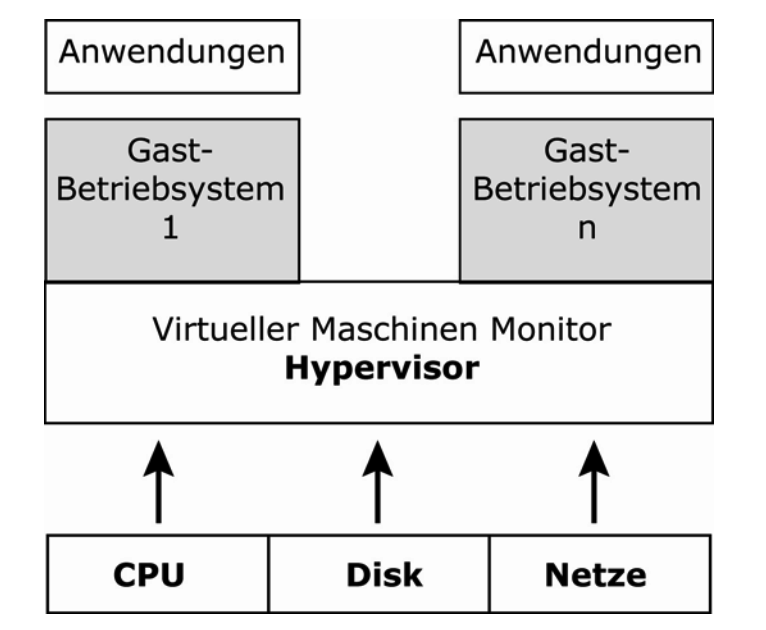
\includegraphics[scale=0.4]{../Bilder/BSVirtualisierung.png}%
	\captionof{figure}[Betriebssystemvirtualisierung]{Betriebssystemvirtualisierung [\cite{SiegertBaumgarten200612}]}%
	\label{fig:Betriebssystemvirtualisierung}% 
 \end{minipage}
\end{center}

\subsection{Hypervisor}\label{subsec:Hypervisor}
Die Benamung des Hypervisors kann von Hersteller zu Hersteller variieren. Bei Microsoft wird er z.B. Hyper-V genannt, w�hrend der Hypervisor bei VMware unter der Bezeichnung ESXi l�uft.
Der Hypervisor, oder in der Literatur auch VMM (Virtual Machine Monitor) genannt, ist die sogenannte abstrahierende Schicht zwischen der tats�chlich vorhanden Hardware und den ggf. mehrfach existierenden Betriebssystemen. Zu sehen in Abbildung \ref{fig:Betriebssystemvirtualisierung}.
Seine prim�re Aufgabe ist die Verwaltung der Host-Ressourcen und deren Zuteilung bei Anfragen der Gastsysteme. L�sen Instruktionen oder Anfagen eines Gastbetriebssystems eine CPU-Exception aus, weil diese im Benutzer-Modus ausgef�hrt werden, f�ngt der Hypervisor diese auf und emuliert die Ausf�hrung der Instruktionen (trap and emulate). Die Ressourcen des Hostsystems werden durch den Hypervisor so verwaltet, dass diese bedarfsgerecht zur Verf�gung stehen, egal ob ein oder mehrere Gastsysteme laufen. Zu seinen Aufgaben z�hlen unter anderem E/A-Zugriffe (insbesondere Hardwarezugriffe), Speichermanagement, Prozesswechsel und System-Aufrufe.\newline
\begin{figure} 
    \subfigure[Bezeichnung der linken Grafik]{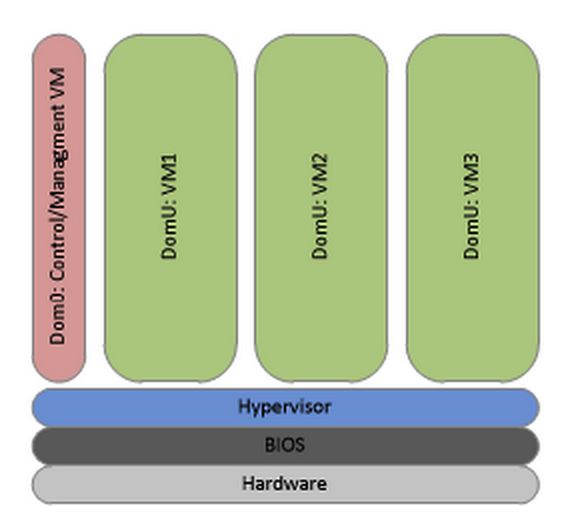
\includegraphics[width=0.49\textwidth]{../Bilder/Hypervisor1.png}} 
    \subfigure[Bezeichnung der rechten Grafik]{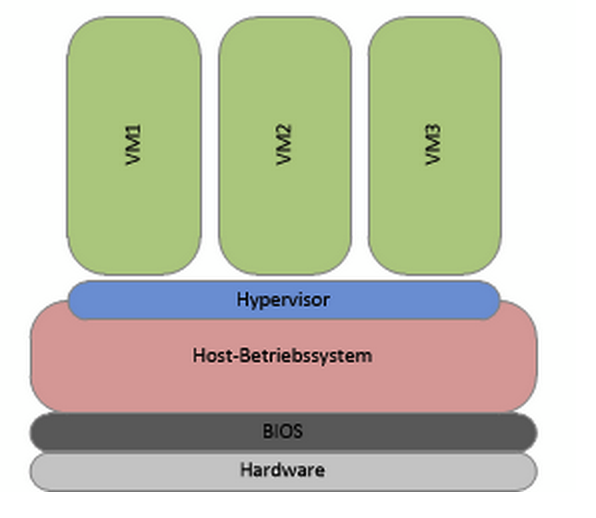
\includegraphics[width=0.49\textwidth]{../Bilder/Hypervisor2.png}} 
\label{fig:KlassifizierungHypervisor}%
\caption{Hypervisor Typ 1 und 2} 
\end{figure} 
\FloatBarrier
Der Hypervisor kann in zwei verschiedene Typen kategorisiert werden:
\begin{description}
\item  [Typ 1 Hypervisor]\hfill \\
arbeitet direkt auf der Hardware und ben�tigt kein Betriebssystem, welches zwischen ihm und der Hardware betrieben wird. Alle dar�ber liegenden virtuellen Maschinen laufen in sogenannten Domains. Weder der Hypervisor noch die anderen Domains sind f�r die jeweilige Domain sichtbar. Die Verwaltung der laufenden Domains wird durch eine priviligierte Domain geregelt, die in der sogenannten 'Dom0' l�uft. Dadurch erh�lt die privilegierte Domain die M�glichkeit andere Domains zu starten, zu stoppen und zu verwalten.\newline
Der Hypervisor Typ-1 verf�gt selbst �ber die n�tigen Ger�tetreiber, um den virtuellen Maschinen sowohl CPU, Speicher als auch I/O zur Verf�gung zu stellen. Durch die wegfallende Schicht, n�mlich dem nicht ben�tigten Betriebssystem, gewinnt der Hypervisor Typ 1 an Performance und reduziert den Ressourcenverbrauch. Siehe Abbildung [\ref{fig:KlassifizierungHypervisor}.a].

\item  [Typ 2 Hypervisor]\hfill \\
l�sst durch seine Bezeichnung als 'Hosted' bereits erahnen, dass der Unterschied zu Typ 1 darin besteht, dass er auf einem Hostsystem aufsetzt. Es muss also eine Schicht implementiert sein, die zwischen dem Hypervisor und der Hardware liegt. Siehe Abbildung [\ref{fig:KlassifizierungHypervisor}.b].\newline
Diese Schicht wird durch ein Betriebssystem realisiert, das dem Hypervisor den Zugang zur Hardware durch die eigenen Hardwaretreiber erm�glicht.
Ist das Betriebssystem mit der Hardware kompatibel, ist transitiv gesehen, der Hypervisor ebenfalls mit installiert- und ausf�hrbar. Dies vereinfacht die Installation gegen�ber dem Hypervisor Typ 1. \newline
Aus Implementierungssicht gibt es f�r beide Hypervisoren Vor- und Nachteile.
F�r einige Bereiche ist die Anforderung eines Betriebssystems nur von Vorteil.
Vor allem, wenn es um Hardware- und Treiber-Kompatibilit�t, Konfigurationsflexibilit�t und vertraute Management-Tools geht.\newline
Auf der anderen Seite kann genau das zum Nachteil gereichen.
Es entsteht nicht nur ein h�herer Management-Aufwand, um das Betriebssystem zu konfigurieren und zu verwalten, auch die Performance und der Sicherheitsaspekt leiden unter dieser zus�tzlichen Schicht f�r das Betriebssystem.
\end{description}

\section{Konfigurationsmanagement-System}\label{sec:Konfigurationsmanagement}
Die Hauptaufgabe eines Konfigurationsmanagement-Systems ist es, eine zuvor definierte Zustandsbeschreibung eines Zielrechners umzusetzen. Dies kann die Installation von Softwarepaketen bedeuten, das Starten oder Beenden von Diensten oder Konfigurationen erstellen/anpassen/entfernen zu lassen. Im Allgemeinen wird dieser Vorbereitungsprozess auch 'provisioning' (zu Deutsch: Provisionieren) genannt und stattet den Zielrechner mit allen Vorraussetzungen f�r seine Aufgaben aus.
In der Regel verwenden Konfigurationsmanagement-System eigene Agenten auf den Zielrechnern, �ber die die Kommunikation abgewickelt und die Zustandsbeschreibung realisiert wird. Neuere Anwendungen wie 'Ansible' (Kapitel \ref{ssec:Ansible}) kommen ohne Agenten aus. Die Kommunikation wird im Falle von Ansible �ber eine SSH-Schnittstelle realisiert.
Pull-basierte Tools, wie beispielsweise 'Puppet' (Kapitel \ref{ssec:Puppet}), fragen in regelm��igen Abst�nden ein zentrales Konfigurations-Repository ab, in dem die jeweils aktuelle Zustandsbeschreibung der Maschine gespeichert ist. Sie sorgen daf�r, dass die �nderungen auf dem Ziel-Client ausgef�hrt werden.
Es spielt keine Rolle, ob das Ziel eine virtuelle Maschine oder eine standard Hardware-Maschine ist. Konfigurationsmanagement-System sind in der Regel dazu f�hig, ganze Gruppen an Rechnern parallel zu bearbeiten und die entsprechenden Zustandsbeschreibungen umzusetzen. 
In dem bereits genannten Beispiel 'Ansible', k�nnen mehrere Rechner simpel in Inventory-Dateien (siehe Listing \ref{lst:InventoryDatei}) als Gruppen zusammengefasst werden. Jede Gruppe erh�lt einzeln die entsprechend vorgesehenen Zustandsbeschreibungen. 

\begin{lstlisting} [caption={Beispiel Inventory-Datei}\label{lst:InventoryDatei},captionpos=t] 
[atomic]
 192.168.100.100
 192.168.100.101
[webserver]
 192.168.1.110
 192.168.1.111
 \end{lstlisting}
Die Integration und Anwendung von Konfigurationsmanagement-Systemen beschleunigt also nicht nur den Aufbau eines oder mehrerer Zielrechner, sondern hilft auch bei der Organisation der Softwareverteilung.

%Quelle: http://www.admin-magazin.de/Online-Artikel/Konfigurationsmanagement-mit-Ansible

\begin{comment}
\section{Begriffserkl�rung}
\item \textbf{Entwicklungsumgebung}\newline
IDE's (integrated development environment) sind Entwicklungsumgebungen, die den Entwickler unterst�tzen, Quellcode zu schreiben und zu bearbeiten. Die g�ngigsten IDE's unterst�tzen meist mehrere Programmiersprachen und helfen dem Entwickler mit n�tzlichen Funktionen, wie  z.B. das aufzeigen von Fehlern im Quelltext. Entwicklungsumgebungen sind in vielen F�llen auch PC's / Server / virtuelle Maschinen, die zum Entwickeln installiert und bereitgestellt werden.
Dort k�nnen neue Funktionalit�ten ausprobiert werden und das bestehende System testweise erweitert werden, ohne in die Produktionslandschaft einzugreifen.
In den folgenden Texten wird der Begriff \textit{Entwicklungsumgebung} als Synonym f�r eine virtuelle Maschine benutzt, die dem Anwender die Freiheit gibt, unkompliziert M�glichkeiten auszutesten und neues auszuprobieren.\newline
		\item \textbf{Aufbau einer Maschine}\newline
\textit{Aufbau einer Maschine} beinhaltet immer das automatische Erstellen und Konfigurieren einer virtuellem Maschine mit Hilfe von VirtualBox und Vagrant.
Das Resultat ist eine virtuelle Maschine mit der Basisinstallation von Ubuntu (32Bit / 64Bit) und \textbf{MEHR INFOS ZU DEM SYSTEM}.
Durch die M�glichkeit des Provisioning kann die Basisinstallation mit Software erg�nzt und Befehle auf der Maschine ausgef�hrt werden.

\end{comment}


\chapter{Anforderungsanalyse}\label{ch:Anforderungsanalyse}
Die Anforderungsanalyse hilft Systemeigenschaften und Systemanforderungen der einzelnen beteiligten Gruppen, auch als Stakeholder bezeichnet,
zu erfassen, zu analysieren und ggf. eine Diskussionsgrundlage zu schaffen. Das resultierende Ergebnis, kann dann wiederum als Grundstein f�r ein zuk�nftiges Lastenheft genutzt werden.

\section{Zielsetzung}\label{Zielsetzung}
"Keine Systementwicklung sollte ohne wenigstens eine halbe Seite schriftliche Ziele angegangen werden. Dabei ist es wichtig, quantifizierbare Angaben aufzuz�hlen, denn Ziele sind Anforderungen auf einer abstrakten Ebene." [\cite{RuppSOPHISTen201410}]\newline\newline
Die zu erstellende Applikation (in den folgenden Kapiteln auch als VM-Builder bezeichnet) soll den Anwender in der Umsetzung und Konfiguration von virtuellen Entwicklungsumgebungen unterst�tzen.
Angestrebte Funktionalit�ten, wie der Aufbau einer Entwicklungsumgebung inklusive der automatisierten Installation von Programmen oder der Austausch von bereits erstellten Entwicklungsumgebungen zwischen beteiligten Benutzern, soll den Anwender in seiner T�tigkeit unterst�tzen. Dabei sind User-Interface und der Funktionsumfang prim�re Ziele. W�hrend die Strukturierung des User-Interfaces hilft, sich mit geringem Zeitaufwand in die Applikation einzuarbeiten, vereinfacht ein �bersichtliches Konfigurationsspektrum die Erstellung der gew�nschten virtuellen Umgebung. Die Konfiguration einer virtuellen Maschine muss auch f�r unerfahrene Nutzer m�glich sein und keine speziellen Kenntnisse voraussetzen.
Alle virtuellen Maschinen, die zu einem Zeitpunkt aktiv sind, sollten in getrennten Instanzen laufen und voneinander unterscheidbar sein. Die Unterscheidbarkeit soll Funktionen wie den Export oder den entfernten Zugriff auf die Maschine unterst�tzen. Diese soll dem Anwender die M�glichkeit schaffen, die gew�nschte virtuelle Maschine zu beeinflussen, indem er die Umgebung abschalten oder zerst�ren kann.
Des Weiteren soll der VM-Builder Unterst�tzung bieten, voneinander abh�ngige Applikationen zu konfigurieren und automatisiert zu installieren.

\section{Stakeholder} \label{STAKEHOLDER}
"\textit{Stakeholder} in Softwareentwicklungsprojekten sind alle Personen (oder Gruppen von Personen) die ein Interesse an einem Softwarevorhaben oder dessen Ergebnis haben." 		 [\cite{Starke201205}]\newline

\begin{table}[h]
\begin{tabular}{|p{4cm} | p{9cm} |}
\hline 
\textbf{Rolle} & Anwender\\ \hline
\textbf{Beschreibung} & Ein Anwender ist ein Benutzer des Systems, ohne administrative Einfl�sse auf die Applikation.\\ \hline
\textbf{Zie}l & Gute Benutzbarkeit, schnell erlernbar, komfortable Steuerung, leichter Aufbau der gew�nschten Umgebung\\ \hline
\end{tabular}
\caption[Stakeholder: Anwender]{Stakeholder: Anwender\footnotemark}
\end{table}\footnotetext{Quelle: Eigene Darstellung}  
\FloatBarrier

\begin{table}[h]
\begin{tabular}{|p{4cm} | p{9cm} |}
\hline 
\textbf{Rolle} & Administrator\\ \hline
\textbf{Beschreibung} & Der Administrator kann die Applikation wie der Anwender nutzen. Er hat erweiterte M�glichkeiten, im Bezug auf die Konfiguration des Systems.\\ \hline
\textbf{Zie}l & Leicht ersichtliche Konfigurationsm�glichkeiten, schnelles auffinden von auftretenden Fehlern, gut protokollierte Fehler\\ \hline
\end{tabular}
\caption[Stakeholder: Administrator]{Stakeholder: Administrator\footnotemark}
\end{table}\footnotetext{Quelle: Eigene Darstellung}  
\FloatBarrier


\begin{comment}
\begin{center}
 \begin{minipage}{\linewidth}
	\centering
	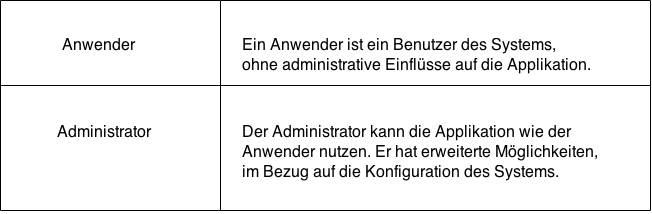
\includegraphics[scale=0.4]{../Bilder/Stakeholder.png}%
	\captionof{figure}[Stakeholderdefinition]{Stakeholder}%
 \end{minipage}
\end{center}
\end{comment}

\section{Funktionale Anforderungen} \label{sec:FunktionaleAnforderungen}
Durch funktionalen Anforderungen werden Kernaufgaben des Systems herausgestellt und beschrieben. Dies beinhaltet dessen Dienste oder Funktionalit�ten, die das System bereitstellen soll. Die Unterpunkte 'FA' listen die einzelnen funktionalen Anforderungen auf und werden in den Use-Cases (Abschnitt \ref{sec:UseCase}) erneut aufgegriffen.\newline\newline
\textbf{Anforderungen - Anwender}
\begin{enumerate}

\item[FA 1.]
Die Applikation muss �ber den Browser ausf�hrbar sein, ohne zus�tzliche lokale Installationen auf Anwenderseite.			
			
\item[FA 2.]	
Die Applikation muss dem Anwender die M�glichkeit bieten, eine virtuelle Maschine zu erstellen.

\item[FA 3.]\label{itm:AUSWAHLMIT}	
M�chte der Anwender auf der virtuellen Maschine Software installiert haben, sollte die Applikation ihm Softwarekomponenten zur Auswahl vorschlagen.

\item[FA 4.] 
Falls der Anwender keine zus�tzliche Software auf der virtuellen Maschine haben m�chte, muss die Applikation entsprechend darauf reagieren k�nnen.

\item[FA 5.] 
M�chte der Anwender zus�tzlich Dateien auf die zu erstellende virtuelle Maschine �bertragen, erm�glicht dieses die Applikation.

\item[FA 6.]\label{itm:Abbild}
M�chte der Anwender eine virtuelle Maschine nach dem Abbild einer bereits im System vorhandenen virtuellen Maschine erstellen, bietet die Applikation Optionen daf�r an.
%\item[FA 5.]
%Die Applikation sollte f�hig sein, dem  Bearbeitungsm�glichkeiten f�r die vorzuschlagenden %Softwarekomponenten anzubieten.

%Es ist dem Anwender m�glich, eine Umgebung inkl. Provisioning zu erstellen, in dem er �ber eine Auswahlliste Softwarekomponenten ausw�hlen kann.
		
%\item[FA 4]	\textbf{Aufbau mit Provisioning inkl. eigener Dateien}\newline
%			Durch das Hochladen eigener Dateien, ist der Anwender in der Lage, Umgebungen aufzubauen inkl. seiner eigens ausgesuchten Dateien/Programme.
%			Dies ist in Kombination mit FA 3 \ref{itm:AUSWAHLMIT} m�glich

\item[FA 7.]\label{itm:autoSpeichern}
Die Applikation sollte durch den Erstellungsprozess die Konfiguration der virtuellen Maschinen automatisch speichern k�nnen.

\item[FA 8.]	
Wenn der Anwender eine virtuelle Maschine erstellen m�chte, muss die Applikation bei wichtigen Konfigurationsschritten f�r den Benutzer sichtbare Statusmeldungen anzeigen. 

\item[FA 9.]	
Treten Fehler bei der Erstellung einer virtuellen Maschine auf, muss das System eine Fehlermeldung ausgeben.

 
\item[FA 10.]	
Die Applikation sollte dem Anwender die Option bieten, virtuelle Maschinen zu exportieren. 

%\item[FA 9.] L�SCHEN !!!
%Die Applikation sollte f�hig sein den Export zu komprimieren.

\item[FA 11.] 
Ist der Export durchgef�hrt worden, muss die Applikation dieses mit einer Meldung auf dem Bildschirm best�tigen.
		
\item[FA 12. \label{Import}]
Die Anwendung muss f�hig sein, Exporte wieder importieren zu k�nnen.
Falls w�hren des Imports Datenfehler auftreten, muss die Anwendung den jeweiligen Fehler (Fehlerbeschreibung) auf dem Bildschirm ausgeben.

\item[FA 13.]	
Ist der Import erfolgreich durchgef�hrt worden, soll die Applikation eine entsprechende Meldung anzeigen.
%Durch den Import von Maschinenkonfiguration wird es dem Anwender erm�glicht, selbst- oder von Kollegen erstellte Umgebungen wieder aufzubauen.


\item[FA 14.]	
Die Applikation soll f�hig sein, anderen Anwendern bereits erstellte virtuelle Maschinen �ber das Internet und das lokale Netzwerk zur Verf�gung zu stellen.

\item[FA 15.]
M�chte der Anwender eine bereits erstellte und laufende virtuelle Maschine beenden, muss die Applikation daf�r eine entsprechende Option bieten.

\item[FA 16.]
Falls der Anwender eine bereits erstellte virtuelle Maschine l�schen m�chte, muss die Applikation ihm daf�r ein Hilfsmittel bereitstellen.	


\end{enumerate}	
\textbf{Anforderungen - Administrator}
	
\begin{enumerate}
\item[FA 17.]
Falls w�hrend des Betriebes der Anwendung �nderungen an der Konfiguration durchgef�hrt werden m�ssen, soll die Applikation dieses �ber eine Konfigurationsseite anbieten.

\item[FA 18.]	
Zu den Konfigurationsm�glichkeiten soll das �ndern des Namens sowie des Speicherorts von Logdateien geh�ren.

\item[FA 19.]	
Falls in den Einstellungen ein Fehler w�hrend der Bearbeitung auftritt, muss die Anwendung eine Fehlermeldung auf dem Bildschirm ausgeben.

\item[FA 20.]	
Die Anwendung sollte dem Administrator die Option bieten, sich den Inhalt von Logdateien anzeigen zu lassen.

\item[FA 21.]
F�r das Hinzuf�gen, �ndern und L�schen von Softwarekomponenten, muss die Applikation eine Oberfl�che bereitstellen.

\item[FA 22.]
Die Applikation muss eine Oberfl�che anbieten, in der Softwarepakete konfiguriert werden k�nnen. Es muss dort m�glich sein, ein neues Softwarepaket anzulegen, Relationen zu anderer Software herzustellen und ggf. Dateien auszuw�hlen und dies als Paket zu speichern.

\item[FA 23.]
Das Erstellen, �ndern und L�schen von Softwarepaketen muss als Option in der Applikation angeboten werden.

\end{enumerate}	
Definition der funktionale Anforderungen nach \cite{RuppSOPHISTen201410}

\section{Use-Cases}\label{sec:UseCase}
Use-Cases (Anwendungsf�lle) helfen, die fachlichen Anforderungen eines Systems zu bezeichnen, indem dort Interaktionen zwischen System und Benutzer dargestellt werden und das System in eine �bersicht seiner Hauptfunktionen gegliedert wird.
Der Business-Use-Case spiegelt dabei ein Gesamtbild aller Funktionalit�ten der Applikation wieder und grenzt diese voneinander ab. Die darauf folgenden System-Use-Cases helfen dabei Hauptfunktionalit�ten zu skizzieren, die sich aus den funktionalen Anforderungen (Kapitel \ref{sec:FunktionaleAnforderungen}) ergeben haben:
\begin{enumerate}
\item Erstellung einer virtuellen Maschine,
\item Export einer vorhandenen Maschine,
\item Import einer zuvor erstellten Maschine,
\item Eine virtuelle Maschine f�r andere Anwender zugreifbar machen (teilen),
\item Software-Abh�ngigkeiten konfigurieren.
\end{enumerate}

\subsection{Business-Use-Case}\label{ssec:BusinessUseCase}
\begin{figure}[htbp]
  \centering
  \fbox{
\includegraphics[scale=0.5]{../Bilder/UseCaseUebersicht.png}
  }
\caption[Business-Use-Case �bersicht]{Business-Use-Case �bersicht\footnotemark}
%\caption{Hypervisor Typ 1 und 2}\footnote{}
\end{figure}\footnotetext{Bildquelle: Eigene Darstellung}  
\FloatBarrier

\subsection{System-Use-Case}

\subsubsection{Use-Case 1 - Virtuelle Maschine erstellen}\label{sssec:UseCase1}
\begin{tabular}{p{4cm} p{10cm}}
\textbf{Bezeichnung} & Virtuelle Maschine erstellen \\
\textbf{Ziel im Kontext} & Erstellung einer virtuellen Maschine \\
\textbf{Akteur} & Anwender \\
\textbf{Ausl�ser} & Der Anwender m�chte eine virtuelle Maschine erstellen. \\
\textbf{Vorbedingung} & Die Anwendung ist installiert und lauff�hig.\newline Der Anwender kann auf die Benutzeroberfl�che zugreifen.\\
\textbf{Nachbedingung} & Der Anwender kann auf eine lauff�hige virtuelle Maschine zugreifen, die seiner Konfiguration entspricht.\\
\textbf{Anforderungen} & FA 2, FA 3, FA 4, FA 5 , FA 7, FA 8, FA 9 \\
\textbf{Erfolgsszenario} & 
 \end{tabular}
\begin{enumerate}
\item Der Anwender startet den VM-Builder �ber den Browser.
\item Der Anwender w�hlt aus, dass er eine neue virtuelle Maschine erstellen m�chte.
\item Der Anwender wird gebeten Konfigurationsparameter f�r die zu erstellende Maschine einzugeben.
\item Die Applikation schl�gt dem Anwender vor, Software mit auf die gew�nschte Maschine zu installieren.
\item Der Anwender kann optional eigene Dateien mit �bertragen lassen.
\item Nach der entsprechenden Auswahl zeigt die Applikation den aktuellen Aufbaustatus der virtuellen Maschine.
\item Die Applikation zeigt dem Anwender die Zugriffsm�glichkeiten f�r die Maschine. an\newline\newline
\end{enumerate}


\subsubsection{Use-Case 2 - Virtuelle Maschine exportieren}
\begin{tabular}{p{4cm} p{10cm}}
\textbf{Bezeichnung} & Virtuelle Maschine exportieren \\
\textbf{Ziel im Kontext} & Export aller notwendigen Konfigurationsdateien, um eine Maschine mit der gleichen Konfiguration erneut erstellen zu k�nnen. \\
\textbf{Akteur} & Anwender \\
\textbf{Ausl�ser} & Der Anwender m�chte eine virtuelle Maschine exportieren. \\
\textbf{Vorbedingung} & Die zu exportierende virtuelle Maschine existiert bereits. \\
\textbf{Nachbedingung} & Der Anwender erh�lt eine gepackte Datei, in der alle n�tigen Daten enthalten sind, die f�r einen erneuten Import n�tig w�ren. \\
\textbf{Anforderungen} & FA 11, FA 12\\
\textbf{Erfolgsszenario} & 
 \end{tabular}
\begin{enumerate}
\item Der Anwender startet den VM-Builder �ber den Browser.
\item Der Anwender w�hlt bei der gew�nschten virtuellen Maschine die Exportfunktion aus.
\item Die Applikation beginnt mit dem Download der ben�tigten Dateien. \newline\newline
\end{enumerate}


\subsubsection{Use-Case 3 - Virtuelle Maschine importieren}
\begin{tabular}{p{4cm} p{10cm}}
\textbf{Bezeichnung} & Virtuelle Maschine importieren \\
\textbf{Ziel im Kontext} & Erstellung einer Maschine aus einem Import. \\
\textbf{Akteur} & Anwender \\
\textbf{Ausl�ser} & Der Anwender m�chte eine virtuelle Maschine importieren. \\
\textbf{Vorbedingung} & Die Anwendung ist installiert und lauff�hig.\newline Der Anwender kann auf die Benutzeroberfl�che zugreifen. \\
\textbf{Nachbedingung} & Die Maschinenkonfiguration konnte importiert werden und eine virtuelle Maschine wurde erstellt. \\
\textbf{Anforderungen} & FA 12, FA 13\\
\textbf{Erfolgsszenario} & 
 \end{tabular}
\begin{enumerate}
\item Der Anwender startet den VM-Builder �ber den Browser.
\item Der Anwender w�hlt die Importfunktion aus und kann die gew�nschte(n) Datei(en) hochladen.
\item Die Applikation zeigt dem Anwender, dass der Import erfolgreich war.
\item Der Anwender kann nun entscheiden, ob er die virtuelle Maschine erstellen lassen m�chte.\newline\newline
\end{enumerate}


\subsubsection{Use-Case 4 - Virtuelle Maschine teilen}
\begin{tabular}{p{4cm} p{10cm}}
\textbf{Bezeichnung} & Virtuelle Maschine teilen \\
\textbf{Ziel im Kontext} & Eine erstellte Maschine �ber das Internet oder das lokale Netzwerk f�r andere Anwender zugreifbar machen.  \\
\textbf{Akteur} & Anwender \\
\textbf{Ausl�ser} & Der Anwender m�chte eine virtuelle Maschine f�r andere Anwender zugreifbar machen. \\
\textbf{Vorbedingung} & Die Anwendung ist installiert und lauff�hig\newline Die zu teilende Maschine ist erstellt. \\
\textbf{Nachbedingung} & Die virtuelle Maschine ist von intern und/oder extern zugreifbar.\\
\textbf{Anforderungen} & FA 14 \\
\textbf{Erfolgsszenario} & 
 \end{tabular}
\begin{enumerate}
\item Der Anwender startet den VM-Builder �ber den Browser.
\item Der Anwender w�hlt die gew�nschte virtuelle Maschine aus und aktiviert die Teil-Option.
\item Die Applikation zeigt dem Anwender die Zugriffsm�glichkeiten auf die virtuelle Maschine.
\end{enumerate}

\subsubsection{Use-Case 5 - Softwarepakete konfigurieren}
\begin{tabular}{p{4cm} p{10cm}}
\textbf{Bezeichnung} & Softwarepakete konfigurieren \\
\textbf{Ziel im Kontext} & Softwarepakete konfigurieren, die andere Software und ggf. das Kopieren/Entpacken von Dateien beinhaltet. \\
\textbf{Akteur} & Administrator \\
\textbf{Ausl�ser} & Eine Installation einer Anwendung, die mehrere Softwarekomponenten ben�tigt.  \\
\textbf{Vorbedingung} & Wissen �ber die zu installierenden Softwarekomponenten. \\
\textbf{Nachbedingung} & Ein Softwarepaket, dass die Konfigurationen des Anwenders beinhaltet und in der Applikation anwendbar ist.\\
\textbf{Anforderungen} & FA 21, FA 22, FA 23 \\
\textbf{Erfolgsszenario} & 
 \end{tabular}
\begin{enumerate}
\item Der Administrator startet den VM-Builder �ber den Browser.
\item Der Administrator navigiert in das Administrationsmen�.
\item Der Administrator erstellt ein neues Softwarepaket.
\item Der Administrator gibt die entsprechenden Optionen wie z.B. Name des Softwarepakets ein.
\item Der Administrator w�hlt die Komponenten aus, die mitinstalliert werden sollen.
\item Der Administrator w�hlt Dateien aus, die auf den Zielrechner kopiert und/oder entpackt werden sollen.
\item Der Administrator speichert das Paket und kann es bei der Installation einer virtuellen Maschine ausw�hlen.
\end{enumerate}


\section{Nichtfunktionale Anforderungen} \label{sec:NFA}
Die Literatur gibt keine einheitliche Definition von nichtfunktionalen Anforderungen vor, aber wie \cite{Burge02} es formulierte, k�nnen durch nichtfunktionale Anforderungen neue L�sungsm�glichkeiten vorgegeben werden oder eine Menge an potentiellen Designentw�rfen, in Bezug auf die Funktionalit�ten, reduziert werden.
Im Wesentlichen gibt es eine begrenze Auswahl an Definitionen und Perspektiven bei nichtfunktionalen Anforderungen, die im Folgenden nach \cite{RuppSOPHISTen201410} zusammengefasst werden.
%von \cite{ChungNixonYuMylopoulos199910} beschrieben:
%Bezogen auf das Design eines Systems sind die nichtfunktionalen Anforderungen f�r den Architekten von besonderer Bedeutung
\begin{enumerate}
\item  \textbf{Technologische Anforderungen}\label{itm:TechnologischeAnforderungen} \newline
Die detailliertere Beschreibung von L�sungsvorgaben oder der Umgebung, in der das System betrieben werden soll, k�nnen und sollen den L�sungsraum f�r die Realisierung des Systems beschr�nken.

\item  \textbf{Qualit�tsanforderungen}\label{itm:Qualit�tsanforderungen}\newline
Qualit�tsanforderungen lassen sich in detailliertere Unterpunkte unterteilen. Dieses kann durch Anwendung von zwei Standards erfolgen: ISO 25000 und ISO 9126. Alledings ist der ISO 9126 Standard in den ISO 25000 �bernommen worden. Beide Standards sollen sicherstellen, dass die Qualit�t des Systems und des Entwicklungsprozesses �ber Qualit�tsanforderungen festgelegt wird.

\item  \textbf{Anforderungen an die Benutzeroberfl�che}\label{itm:AnforderungenAnDieBenutzeroberfl�che}\newline
Die Anforderungen, die festlegen, wie sich die Anwendung dem Benutzer darstellt, werden unter 'Anforderungen an die Benutzeroberf�che' zusammengefasst.
         		
\item  \textbf{Anforderungen an die sonstigen Lieferbestandteile}\newline
Alle Produkte, die zu dem System oder der Anwendung geliefert werden m�ssen, wie z.B. ein Handbuch oder Quellcode, werden unter 'Anforderungen an die sonstigen Lieferbestandteile' beschrieben.

\item  \textbf{Anforderungen an durchzuf�hrende T�tigkeiten}\newline
Die 'Anforderungen an durchzuf�hrende T�tigkeiten' beeinflussen T�tigkeiten, wie Wartung oder Support, die der Entwicklung nachgelagert sind.

\item  \textbf{Rechtliche-vertragliche Anforderungen}\newline
'Rechtliche-vertragliche Anforderungen' beschreiben die Regelungen, die zwischen Auftraggeber und Auftragnehmer vor der Entwicklung des Systems oder deren Anwendung, festgelegt werden m�ssen.
\end{enumerate}
\pagebreak
Im Folgenden werden die nichtfunktionalen Anforderungen hinsichtlich der Punkte \ref{itm:TechnologischeAnforderungen} 'Technologische Anforderungen'  und \ref{itm:AnforderungenAnDieBenutzeroberfl�che} 'Anforderungen an die Benutzeroberfl�che' betrachtet.

\subsubsection{Technologische Anforderungen}\label{sssec:TechnologischeAnforderungen}
\begin{enumerate}
\item Das f�r den Betrieb der Anwendung zugrunde liegende Betriebssystem muss Ubuntu 12.04 oder h�her sein.
\item Die Anzahl der gleichzeitig laufenden virtuellen Umgebungen, liegt maximal bei 10.	
\item Die Kommunikation zwischen Frontend und Backend muss nicht verschl�sselt ablaufen.
\item Softwareupdates der benutzten Softwarekomponenten m�ssen mit R�cksprache des Entwicklers erfolgen.
\end{enumerate}
\subsubsection{Qualit�tsanforderungen}
\begin{enumerate}
\item Die Installation und Inbetriebnahme der Anwendung sollte �ber einen automatischen Installationsprozess erfolgen.
\item Die Anwendung sollte zu 99,0 Prozent der Zeit lauff�hig sein.
\item Jeder auftretende Fehler ist eindeutig identifizierbar und nachvollziehbar.
\item �nderungen am vorgeschlagenen Softwarebestand m�ssen innerhalb von <10 Sekunden in der Anwendungsoberfl�che sichtbar sein.		
\item Falls das Betriebssystem auf eine h�here Version aktualisiert werden soll, muss dieses ohne �nderungen des Quellcodes der Anwendung vorgenommen werden k�nnen.
\item Soll ein anderer Provisionierer verwendet werden, muss der Aufwand des Austausches bei unter f�nf Personentagen liegen.		
\item Wird angedacht weitere Grundfunktionalit�ten zu implementieren, soll dieses m�glichst unkompliziert erfolgen.		
\item Der Zeitaufwand f�r den Import von virtuellen Maschinen sollte <10 Minuten betragen.
\item Die Zeit des Exports einer virtuellen Maschine sollte <5 Minuten betragen.\end{enumerate}

\subsubsection{Anforderungen an die Benutzeroberfl�che}
\begin{quote}
"Mit Anforderungen an die Benutzungsoberfl�che [...] wird eine Menge von Faktoren beschrieben, die sich mit dem visuellen, akustischen oder auch haptischen Erscheinen und der Bedienung des Systems befassen. Sie erg�nzen die funktionalen Anforderungen, die sich an der Oberfl�che zeigen und spezifizieren, wie diese funktionalen Anforderungen zu erscheinen haben." \cite{Sophisten13}
\end{quote}
\begin{enumerate}
\item Ein Benutzer ohne Vorkenntnisse muss bei der erstmaligen Verwendung des VM-Builders innerhalb von maximal 10 Minuten in der Lage sein, die gew�nschte Funktionalit�t zu lokalisieren und zu verwenden.

\item Der VM-Builder sollte einen Oberfl�chendialog f�r die Verwaltung der virtuellen Maschinen bereitstellen. Die folgenden Bezeichnungen, die Art der abgebildeten Elemente, deren G��e und Anordnung sind keine Umsetzungsanforderung. (Siehe Abbildung \ref{fig:Manage}). Prim�r steht eine �bersicht der erstellten virtuellen Maschinen im Vordergrund, inklusive derer verf�gbaren Optionen und Statusinformationen.\newline
\begin{figure}[htbp]
  \centering
  \fbox{
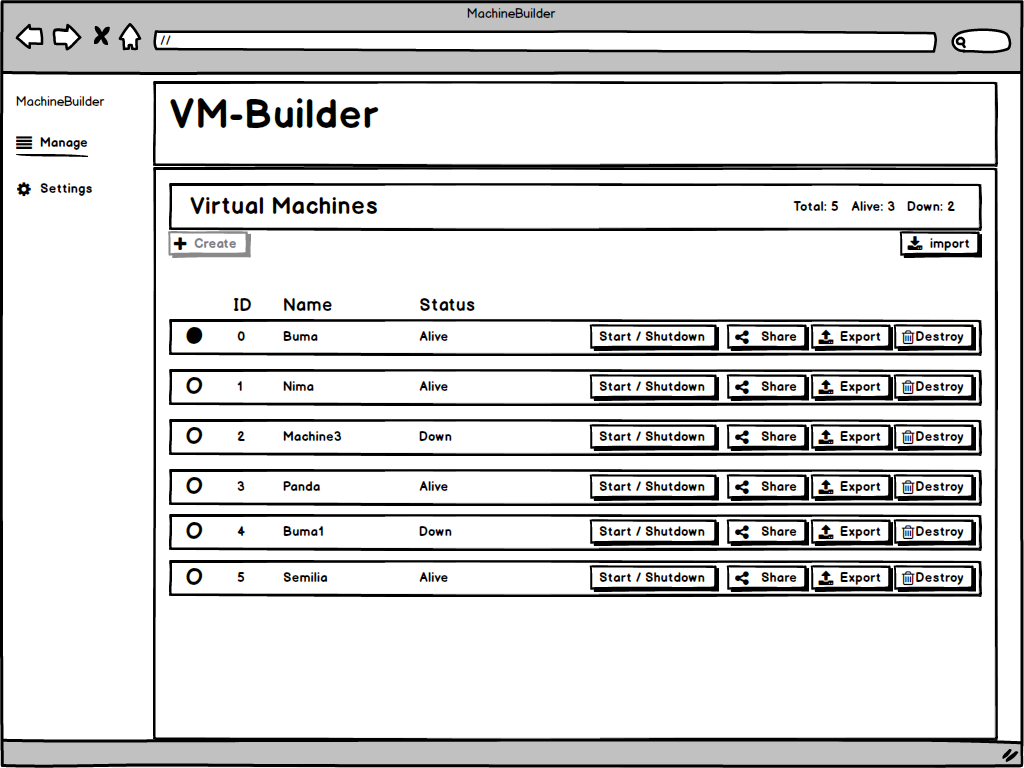
\includegraphics[width=0.5\textwidth]{../Bilder/Mockups/Manage.png}
  }
\caption[Entwurf der Verwaltungsoberfl�che]{Entwurf der Verwaltungsoberfl�che\footnotemark}
\label{fig:Manage}
\end{figure}\footnotetext{Bildquelle: Eigene Darstellung}  
\FloatBarrier
\newpage
\item Der VM-Builder sollte den Oberfl�chendialog 'Virtuelle Maschine erstellen' mit den folgenden Bezeichnungen und der Art der abgebildeten Elemente darstellen (siehe Abbildung \ref{fig:Create1} und \ref{fig:Create2}). Keine umzusetzenden Anforderungen sind die genaue Gr��e und die Anordnung der einzelnen Elemente.
Abbildung \ref{fig:Create1} zeigt die Men�f�hrung des geleiteten Aufbaus einer virtuellen Maschine mit Eingabem�glichkeiten. Abbildung \ref{fig:Create2} zeigt den nachfolgenden Auswahlprozess an Softwarekomponenten.
Zu beachten ist, dass die Eingabe der optionalen- und Pflichtparameter gegeben ist sowie die Auswahlm�glichkeit an Softwarekomponenten.
\begin{comment}
\begin{figure} 
    \subfigure[Enwurf der Aufbauoberfl�che - Eingabe Parameter]{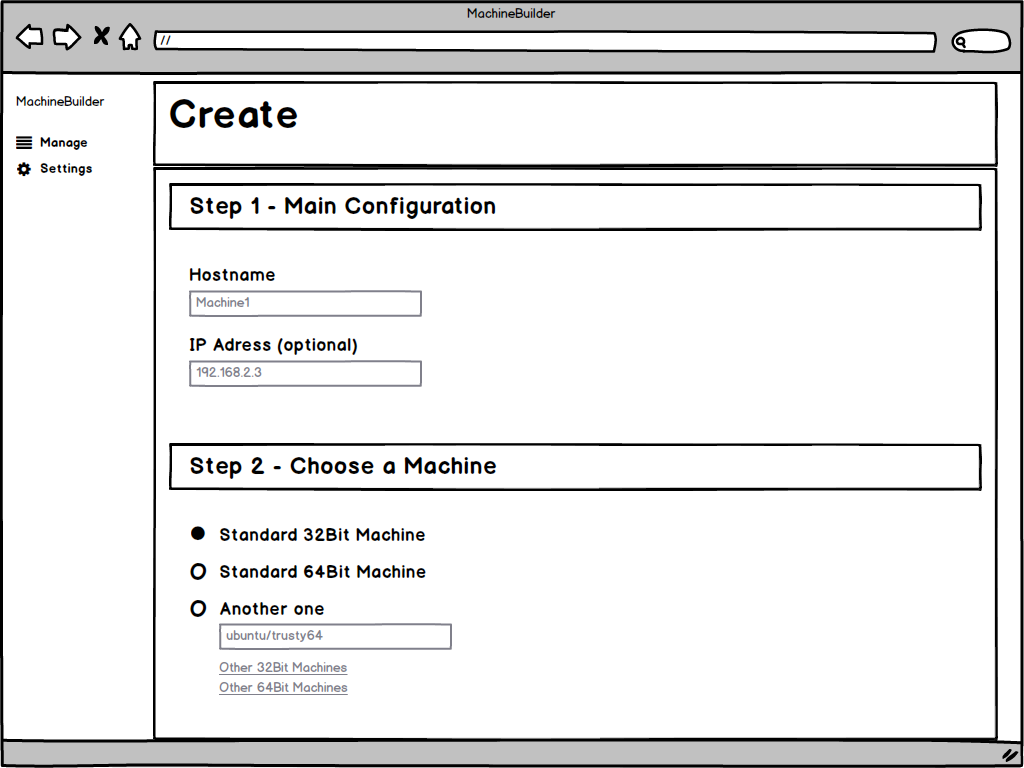
\includegraphics[width=0.49\textwidth]{../Bilder/Mockups/CreatePage1.png}} 
    \subfigure[Enwurf der Aufbauoberfl�che - Auswahl der Softwarekomponenten]{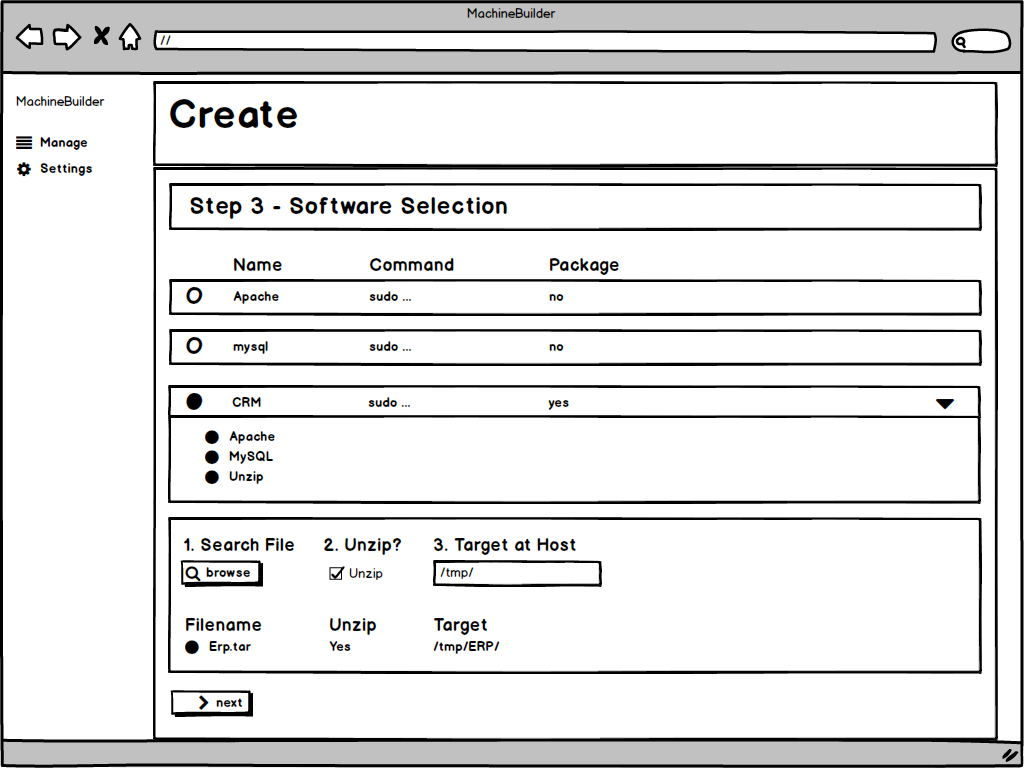
\includegraphics[width=0.49\textwidth]{../Bilder/Mockups/CreatePage12.png}} 
  \caption[Enwurf der Aufbauoberfl�che]{Enwurf der Aufbauoberfl�che\footnotemark}
\label{fig:Create1}
\end{figure}\footnotetext{Bildquelle: Eigene Darstellung}  
\FloatBarrier
\end{comment}

\begin{figure}[htbp]
  \centering
  \fbox{
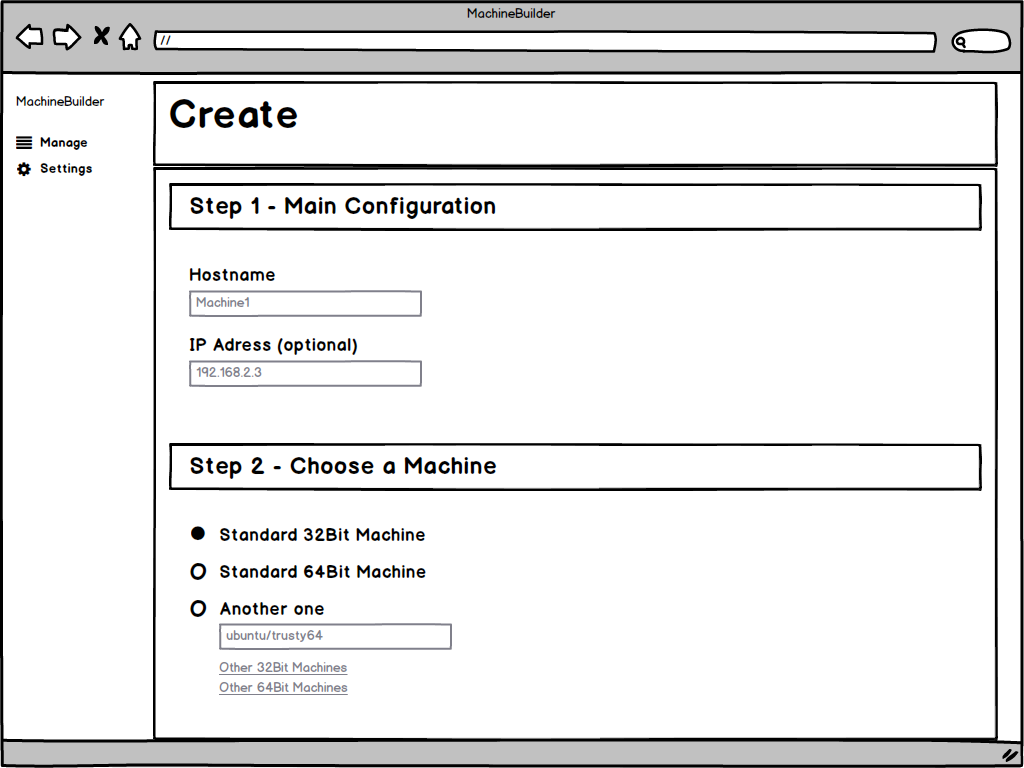
\includegraphics[width=0.5\textwidth]{../Bilder/Mockups/CreatePage1.png}
  }
  \caption[Enwurf der Aufbauoberfl�che - Eingabe Parameter]{Enwurf der Aufbauoberfl�che - Eingabe Parameter\footnotemark}
\label{fig:Create1}
\end{figure}\footnotetext{Bildquelle: Eigene Darstellung}  
\FloatBarrier

\begin{figure}[htbp]
  \centering
  \fbox{
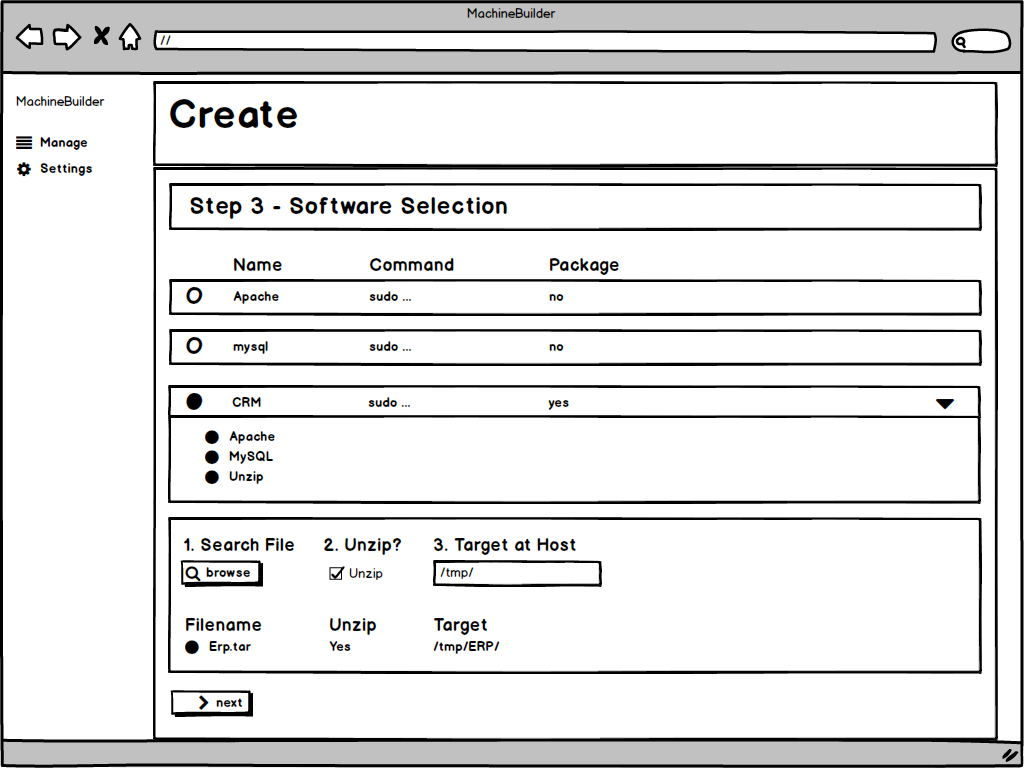
\includegraphics[width=0.5\textwidth]{../Bilder/Mockups/CreatePage12.png}
  }
  \caption[Enwurf der Aufbauoberfl�che - Auswahl der Softwarekomponenten]{Enwurf der Aufbauoberfl�che - Auswahl der Softwarekomponenten\footnotemark}
\label{fig:Create2}
\end{figure}\footnotetext{Bildquelle: Eigene Darstellung}  
\FloatBarrier


\item Der VM-Builder sollte den Oberfl�chendialog 'Sharing' mit den folgenden Bezeichnungen und der Art der abgebildeten Elemente darstellen (siehe Abbildung \ref{fig:Share}). Keine umzusetzenden Anforderungen sind die genaue Gr��e und die Anordnung der einzelnen Elemente. Um die Oberfl�che �bersichtlich zu halten, soll der Anwender nur n�tige Informationen erhalten, die zur Weitergebe an Dritte ben�tig werden. Dieses w�ren z.B. Konnektivit�tsm�glichkeiten und Informationen zur geteilten virtuellen Maschine.
\begin{figure}[htbp]
  \centering
  \fbox{
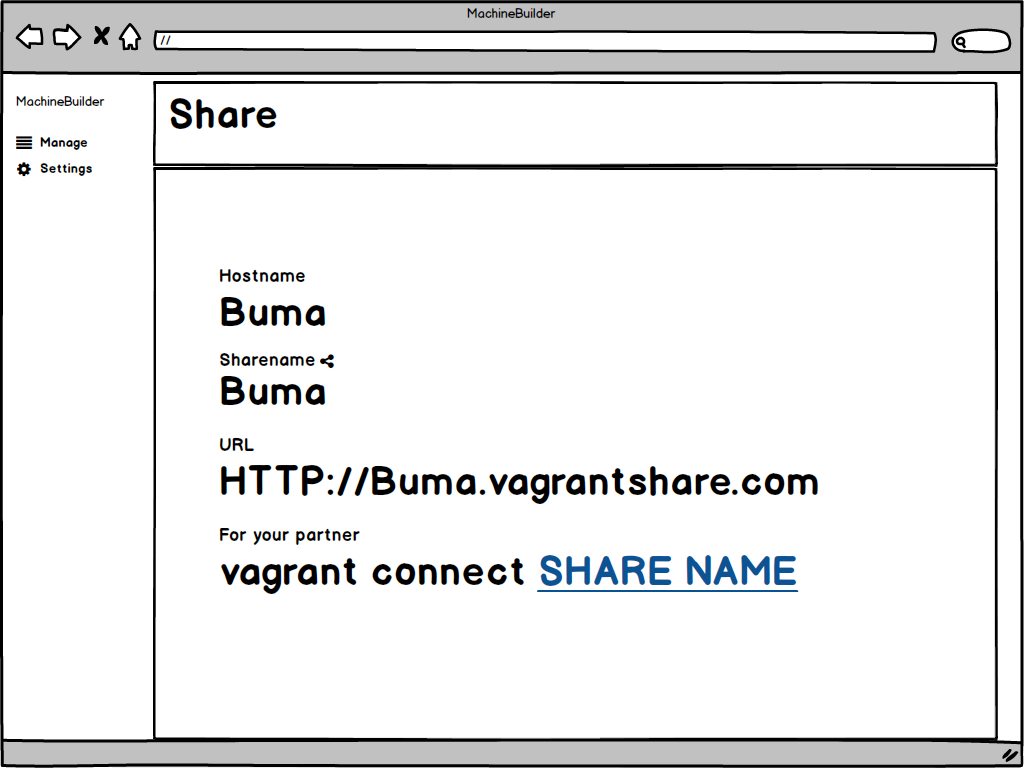
\includegraphics[width=0.5\textwidth]{../Bilder/Mockups/Share.png}
  }
\caption[Entwurf der Sharing-Oberfl�che]{Entwurf der Sharing-Oberfl�che\footnotemark}
\label{fig:Share}
\end{figure}\footnotetext{Bildquelle: Eigene Darstellung}  
\FloatBarrier
\pagebreak
\item Der VM-Builder sollte den Oberfl�chendialog 'Export' besitzen. Durch den Export sollen, von einer zuvor ausgew�hlten virtuellen Maschine, alle n�tigen Konfigurationsdateien exportiert werden k�nnen. In Abbildung \ref{fig:MockExport} wird ein exemplarischer Aufbau der Webansicht gezeigt.
\begin{figure}[htbp]
  \centering
  \fbox{
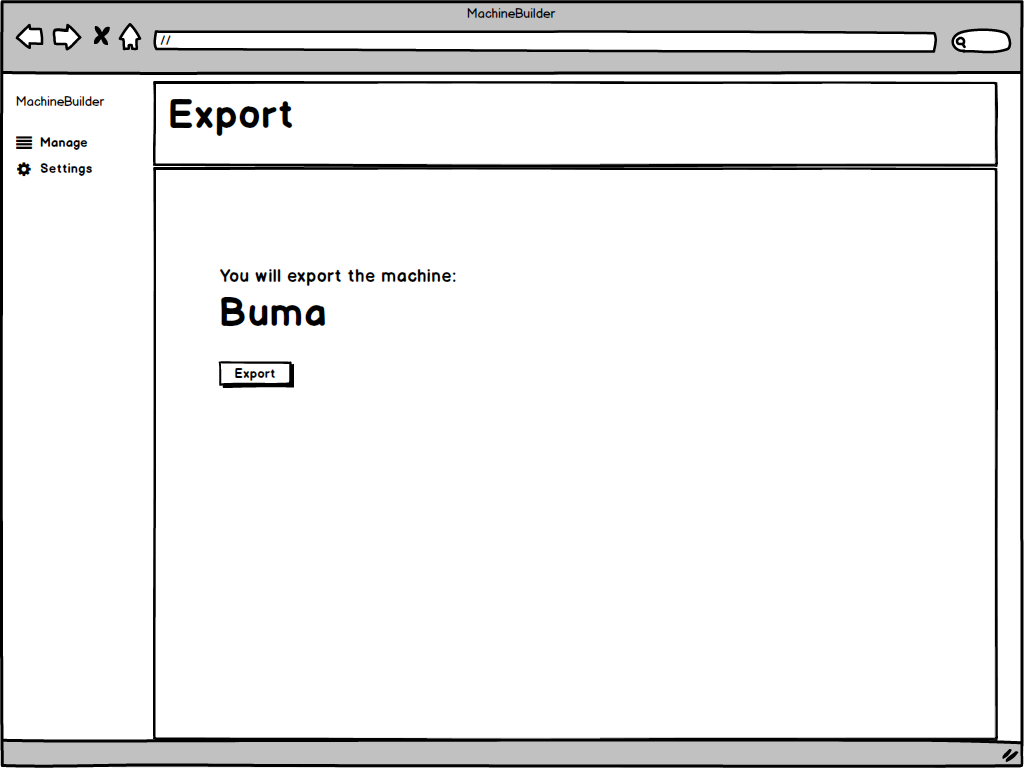
\includegraphics[width=0.5\textwidth]{../Bilder/Mockups/Export.png}
  }
  \caption[Entwurf der Export-Oberfl�che]{Entwurf der Export-Oberfl�che\footnotemark}
\label{fig:MockExport}
\end{figure}\footnotetext{Bildquelle: Eigene Darstellung}  
\FloatBarrier
  

\item Der VM-Builder sollte den Oberfl�chendialog 'Import' besitzen, mit dem der Anwender zuvor exportierte Dateien wieder importieren kann. So sollen Schaltfl�chen zum Ausw�hlen der ben�tigten Dateien angeboten werden. Eine Entwurf der Oberfl�che wird unter Abbildung \ref{fig:MockImport} gezeigt.
\begin{figure}[htbp]
  \centering
  \fbox{
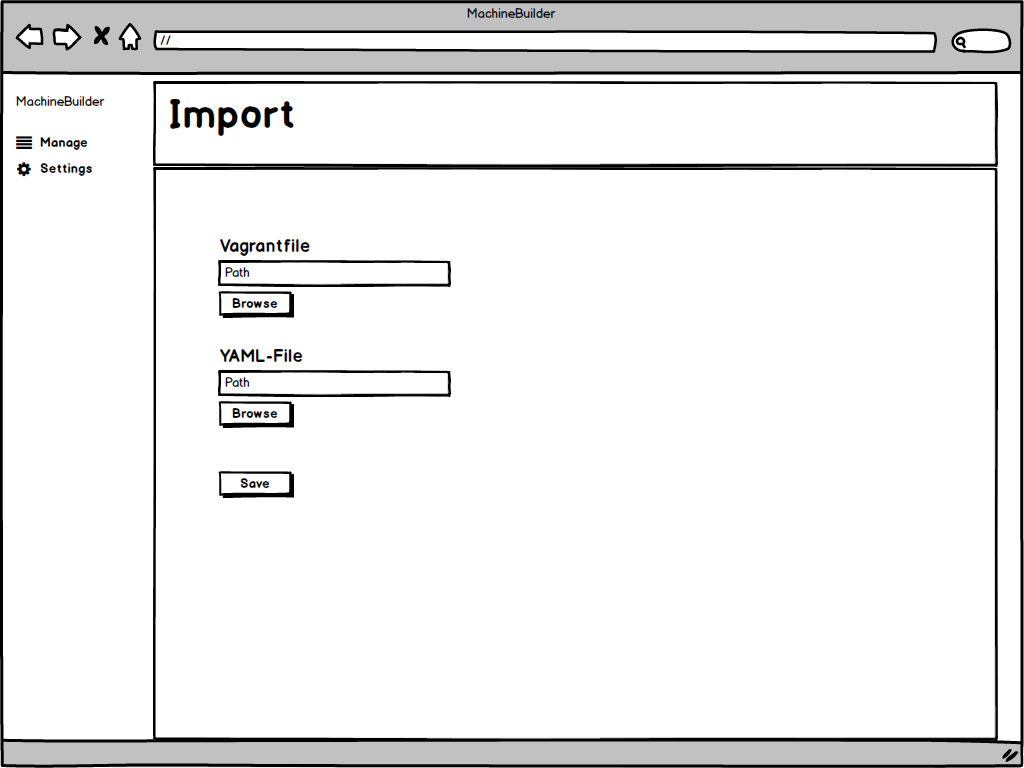
\includegraphics[width=0.5\textwidth]{../Bilder/Mockups/Import.png}
  }
\caption[Entwurf der Import-Oberfl�che]{Entwurf der Import-Oberfl�che\footnotemark}
\label{fig:MockImport}
\end{figure}\footnotetext{Bildquelle: Eigene Darstellung}  
\FloatBarrier

\item Der VM-Builder sollte den Oberfl�chendialog 'Einstellung' besitzen. Die Einstellungen sollen dem Anwender eine generelle �bersicht �ber Applikations-Konfigurationen geben. Zudem soll dort der Inhalt von Log-Dateien einsehbar sein und Softwarekomponenten / Softwarepakete hinzugef�gt werden k�nnen. Die folgenden Entw�rfe (Abbildungen: \ref{fig:MockSettings}, \ref{fig:MockLog}, \ref{fig:MockSoftwarekomponenten}) zeigen Vorschl�ge der einzelnen Seite des Men�s
\begin{figure}[htbp]
  \centering
  \fbox{
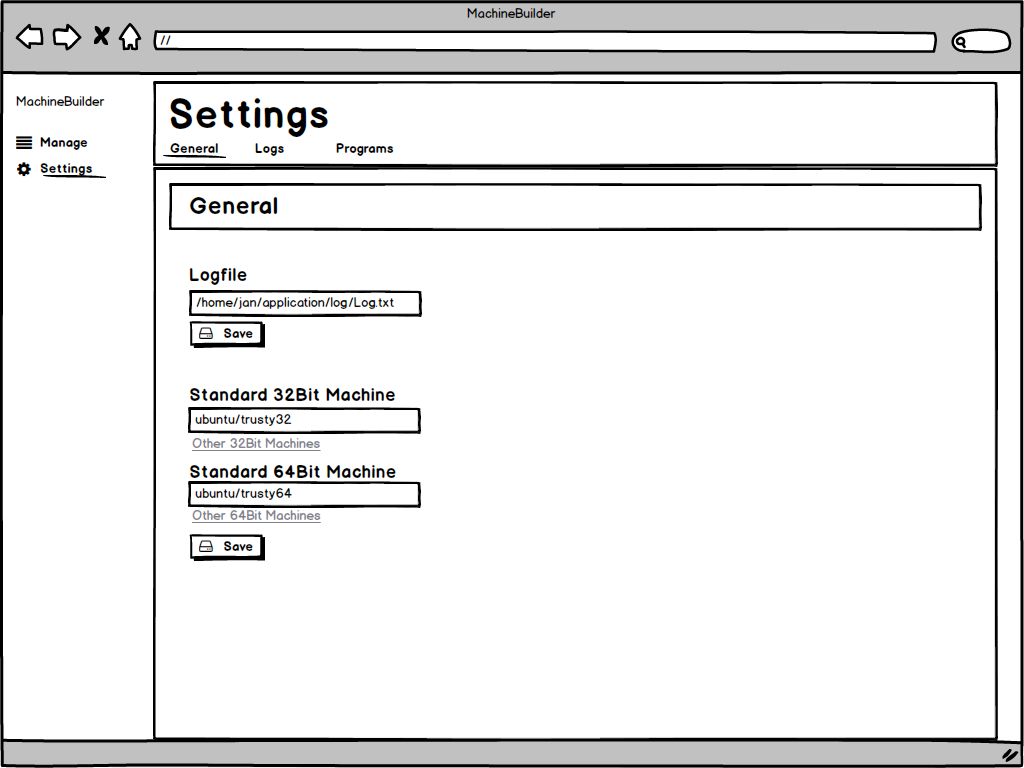
\includegraphics[width=0.5\textwidth]{../Bilder/Mockups/SettingsPage1_1_2.png}
  }
\caption[Entwurf der Einstellungen - Generelle Konfiguration]{Entwurf der Einstellungen - Generelle Konfiguration\footnotemark}
\label{fig:MockSettings}
\end{figure}\footnotetext{Bildquelle: Eigene Darstellung}  
\FloatBarrier


\begin{figure}[htbp]
  \centering
  \fbox{
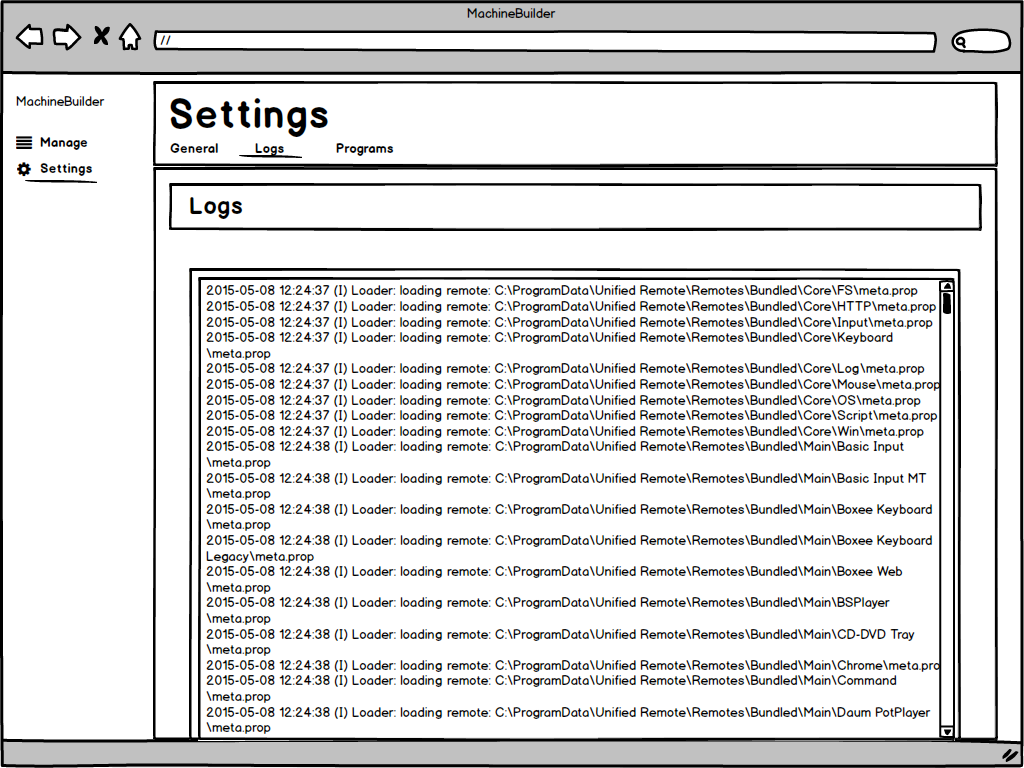
\includegraphics[width=0.5\textwidth]{../Bilder/Mockups/Settings-Logs.png}
  }
\caption[Entwurf der Einstellungen - Logdatei]{Entwurf der Einstellungen - Logdatei\footnotemark}
\label{fig:MockLog}
\end{figure}\footnotetext{Bildquelle: Eigene Darstellung}  
\FloatBarrier


\begin{figure}[htbp]
  \centering
  \fbox{
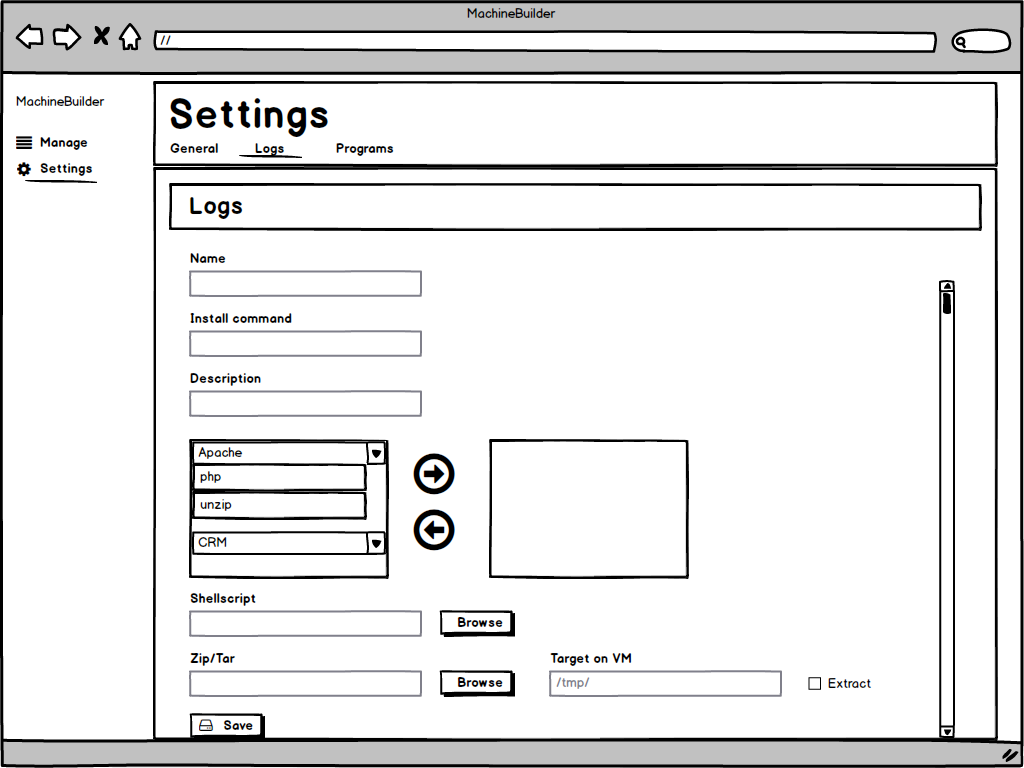
\includegraphics[width=0.5\textwidth]{../Bilder/Mockups/Settings-Programs.png}
  }
\caption[Entwurf der Einstellungen - Softwarekomponenten hinzuf�gen]{Entwurf der Einstellungen - Softwarekomponenten hinzuf�gen}
\label{fig:MockSoftwarekomponenten}
\end{figure}\footnotetext{Bildquelle: Eigene Darstellung}  
\FloatBarrier  
 \end{enumerate}

\pagebreak
\section{Randbedingungen}\label{sec:Randbedingungen}
Um anwendungs�- und problembezogene Entwurfsentscheidungen treffen zu k�nnen, werden Faktoren analysiert, die die Architekturen der Anwendung beeinflussen oder einschr�nken k�nnen. Dieses geschieht �ber die im Vorfeld formulierten Anforderungen.
Laut \cite{Starke201401} werden diese Einflussfaktoren und Randbedingungen in folgende Kategorien unterteilt:
\begin{itemize}
\item Organisatorische und politische Faktoren: Manche solcher Faktoren wirken auf ein be�stimmtes System ein, w�hrend andere eine Vielzahl an Projekten eines Unternehmens beeinflussen k�nnen. [\cite{RechtinMaier200006}] charakterisierten diese Faktoren als 'facts of life'.
\item Technische Faktoren: Durch diese wird das technische Umfeld gepr�gt und entsprechend eingeschr�nkt. Diese betreffen nicht nur die Ablaufumgebung des zu entwickelnden Systems, sondern umfassen auch die technischen Vorgaben f�r die Entwicklung, einzusetzender Software und vorhandener IT-Systeme. [\cite{Starke201401}]
\end{itemize}
Da weder organisatorischen, noch politischen Faktoren auf dieses Projekt Einfluss haben, werden diese nicht weiter betrachtet. 
\pagebreak
\subsection{Technische Randbedingungen}\label{subsec:TechnischeRandbedingungen}
\begin{table}[h]
\begin{tabular}{|p{4cm} | p{9cm} |}
\hline 
\textbf{Randbedingungen} &\textbf{Erl�uterung}\\ \hline
Server Hardware & Die Leistung des Servers sollte entsprechend der Anforderungen
gen�gen. Es muss m�glich sein, mehrere virtuelle Maschinen gleichzeitig laufen zu lassen, ohne das es die einzelnen Maschinen beeinflusst.\\ \hline
Server Betriebssystem & Die L�sung sollte auf einem Ubuntu Server 64Bit
installiert und betrieben werden.\\ \hline
Implementierung in Ruby & Implementierung der Anwendung erfolgt in Ruby mit dem
Framework Sinatra. Da keine seperate Frontend-Kommunikation ben�tigt wird, bietet sich Ruby als Backend-Sprache an. Entwickelt wird in der Version 1.9, welche als stabil gilt.\\ \hline
Fremdsoftware & Fremdsoftware die hinzugezogen wird, sollte idealerweise frei verf�gbar und kostenlos sein. Es sollte drauf geachtet werden, dass die Software etabliert ist und der Fokus auf eine stabile Version gelegt wird.\\ \hline
Web-Frontend & Die Kompatibilit�t zu allen g�ngigen Browsern wird nicht weiter betrachtet. Optimiert wird ausschlie�lich f�r Mozilla Firefox.\\ \hline
\end{tabular}
\caption[Technische Randbedingungen]{Technische Randbedingungen\footnotemark}
\end{table}\footnotetext{Quelle: Eigene Darstellung}  
\FloatBarrier

\section{Vergleichbare Anwendungen}
Wenn es um den Aufbau und die Verwaltung von virtuellen Maschinen geht, steht eine Vielzahl an unterschiedlichster Software zum Angebot. Das Spektrum reicht von der Administration �ber Cloud-Dienste, dem Einsatz von Open-Source-Software, um ganze Rechenzentren zu verwalten oder dem Aufbau von virtuelle Maschinen im privaten Umfeld. Um einen kleinen �berblick �ber popul�re Open-Source-Anwendungen zu erhalten, werden im nachfolgenden Teil zwei Anwendungen vorgestellt, die �hnliche Aufgaben wie der VM-Builder �bernehmen k�nnten. Im Anschluss wird in einem Zwischenfazit (Abschnitt \ref{ssec:FazitVergArbeiten}) kurz erl�utert, wieso die beschriebene Software nicht f�r den Einsatz geeignet ist.

\subsection{OpenNebula}
%OpenNebula ist eine Open Source L�sung, die Cloud basierend ist und unter Verwendung verschiedener Industriestandards eine hochverf�gbare, skalierbare Virtualisierungplattform zur Verf�gung stellt. \cite{Netways:2015:Online}. 
OpenNebula ist eine Open-Source-Cloud L�sung, die sich selbst als ein 'Open-Source-\\Industriestandard zur Virtualisierung von Rechenzentren' bezeichnet [\cite{Hock12}] und hochverf�gbare, skalierbare Virtualisierungsplattformen zur Verf�gung stellt.
Als eine Art IaaS kann OpenNebula die zentrale Administration und �berwachung von virtuellen Systemen �bernehmen. Kommt es zu Ausf�llen von Komponenten kann OpenNebula automatisch einen Neustart auf einem anderen Hostsystem ausf�hren. Zudem sind dynamische Erweiterungen der Hardwareressourcen m�glich. Die Kernkompetenzen liegen dabei auf schon vorhandenen Systemen im Bereich Virtualisierung, Speicherung und Vernetzung.
OpenNebula kann optimal als Werkzeug f�r die Integration vorhandener Systeme verwendet werden, da es diverse M�glichkeiten zur Wartung und Skalierung der gegebenen Infrastruktur zur Verf�gung stellt.\newline
Auch wenn OpenNebula sich selbst in das Enterprise Segment kategorisiert\footnotemark\footnotetext{Quelle: \cite{opennebula:2015:Online}}, ist es jedoch auch f�r kleinere Organisationen praktikabel. Durch die Installation von wenigen Komponenten und die Steuerung �ber nur ein Frontend, macht die Steuerung und Konfiguration komfortabel.

\subsection{OpenStack}
Der Ursprung von OpenStack liegt in einer Kooperation zwischen Rackspace (ein US-Webhoster) und der NASA, die versuchten eine L�sung zu finden, um Rechenkapazit�t an einer zentralen Stelle zu b�ndeln und einzelnen Abteilungen ben�tigte Ressourcen nach Bedarf anzubieten. Nachdem die NASA das Projekt abgegeben hat und diverse IT-Unternehmen OpenStack weiterentwickelten, ist die L�sung ein fester Bestandteil des Portfolios diverser bekannter Linux-Anbieter geworden.
Die Struktur von OpenStack besteht aus einer Vielzahl an Komponenten, die alle unterschiedlich weit entwickelt sind. W�hrend 'Keystone', welches oft als Hauptkomponente von OpenStack bezeichnet wird, als stabil und gut gewartet gilt, liegen neuere Komponenten noch teilweise hinter den Erwartungen der mei�ten Anwender. Ansonsten bietet OpenStack Administratoren ein gro�es Spektrum an Werkzeugen, um ihre Cloud-Computing Umgebung zu verwalten. Durch die vielf�ltigen Einsatzm�glichkeiten und die gro�e Auswahl an Optionen, ist OpenStack ein guter 'Allrounder', mit Defiziten in der Einarbeitungszeit. [\cite{Golem:2015:Online}]
\pagebreak
\subsection{Res�mee}\label{ssec:FazitVergArbeiten}
Eines der wichtigen Merkmale von OpenNebula ist der Schwerpunkt auf Rechenzentrumsvirtualisierung inklusive bestehender Infrastruktur wodurch dieses mehr oder weniger im Enterprise-Cloud-Computing angesiedelt wird, OpenStack dagegen ein Vertreter des Public-Cloud-Computing ist. Einer der Vorteile von OpenNebula ist, dass sich eigene VM-Images per Knopfdruck auf Virtualisierungsservern und dem dazugeh�rigen Storage instanziieren lassen und Zuweisungen wie IP, Load-Balancing und Speicherplatz von der eigenen Verwaltungssoftware �bernommen werden. Zudem kommt eine �bersichtliche Steuerung, die F�higkeit mehrere hundert Server / virtuelle Maschinen verwalten zu k�nnen und die Eigenschaft verh�ltnism��ig einfach in eine bestehende Infrastruktur integriert zu werden. OpenStack versucht f�r alle alles anzubieten und kommt daher mit einer Vielzahl an unterschiedlichen Komponenten daher, die schnell un�bersichtlich werden k�nnen.
Das Komponentensystem bringt aber auch den Vorteil mit sich, nur Komponenten zu verwenden, die ben�tigt werden. So wird im Grunde mehr Flexibilit�t und die Chance auf Kostenreduzierung erreicht.\newline
F�r die Verwaltung von virtuellen Maschinen und Infrastrukturen sind beide Applikationen mehr als geeignet. Allerdings fehlt bei beiden die M�glichkeit direkt Software mit aufzuspielen. Zudem sind beide Anwendungen f�r den anvisierten Verwendungszweck zu umfangreich in ihren Funktionalit�ten und bringen eine zu hohe Einarbeitungszeit mit sich.


\section{Zusammenfassung}
%Die Anforderungsanalyse fasste im Abschnitt \ref{Zielsetzung} die Funktionalit�t der Applikation zusammen. 
In der Anforderungsanalyse wurde in Abschnitt \ref{Zielsetzung} ein �berblick �ber die Ziele des VM-Builders geschaffen. Danach wurden die Stakeholder inklusive ihrer Beschreibung und Ziele definiert, wodurch die Analyse der funktionalen Anforderungen in Abschnitt \ref{sec:FunktionaleAnforderungen} strukturiert wurde. 
Das Ergebnis der funktionalen Anforderung stellte die Kernpunkte der Applikation heraus, die sich wie folgt ergaben:
\begin{enumerate}
\item Die Erstellung einer virtuellen Maschine,
\item Der Export von Maschinen,
\item Der aus dem Export resultierende Import,
\item Die M�glichkeit virtuelle Maschinen mit anderen zu teilen (Sharing),
\item Die Konfiguration von Softwarepakete, um Abh�ngigkeiten zu anderen Softwarekomponenten zu definieren.
\end{enumerate}
Diese Punkte wurden in Abschnitt \ref{sec:UseCase} als Use-Caseszenarien detaillierter in den Kontext des VM-Builders gestellt. Die nichtfunktionalen Anforderungen (siehe Abschnitt \ref{sec:NFA}) bestimmen die Qualit�tsmerkmale der Applikation und ergaben die ersten Anforderungen an die Oberfl�che (siehe Abschnitt \ref{itm:AnforderungenAnDieBenutzeroberfl�che}). Zuletzt wurden die Randbedingungen betrachtet, um Einfluss- und einschr�nkende Faktoren zu finden, die sich auf die Architektur der Applikation beziehen k�nnen.
Die insgesamt geschaffenen Anforderungen werden im folgenden Kapitel \ref{ch:Evaluation}. ('Evaluation') als Grundlage f�r die Recherche nach Produkten verwendet, die f�r den VM-Builder nutzbar sind. Die Ergebnisse aus der Anforderungsanalyse und der Evaluation schaffen zudem eine Grundlage f�r den Entwurf in Kapitel (Kapite \ref{ch:Entwurf}).


\chapter{Evaluation}\label{ch:Evaluation}
Um herauszufinden, ob und welche Softwareprodukte der Anwendung hinzugef�gt werden k�nnen, muss eine Evaluation der vorhanden Produkte, die auf dem Markt sind durchgef�hrt werden durch eine Marktrecherche.
Es ist zu eruieren, ob gew�nschte Funktionalit�ten unter Verwendung der technischen Randbedingungen aus Kapitel \ref{subsec:TechnischeRandbedingungen} - Unterpunkt 'Femdsoftware', von externen Softwarekomponenten unterst�tzt oder sogar durchgef�hrt werden k�nnen, die etabliert und kostenlos sind.

\section{Virtualisierungsprodukte}
Virtualisierungsprodukte oder Tools helfen virtuelle Maschinen f�r tempor�re Zwecke aufzubauen. Beispielsweise um ein alternatives Betriebssystem zu testen, Softwareprodukte auszuprobieren oder Entwicklungsumgebungen zu erstellen.
Die wohl derzeit (Stand Mitte 2015) bekanntesten und etabliertesten Virtualisierungsl�sungen werden von drei verschiedenen Herstellern pr�sentiert und zum Teil als Freeware angeboten.
\begin{enumerate}
\item \textbf{VMware Player / Plus}\newline
Preiswerte Virtualisierungsl�sung f�r Unternehmen. 
Source-Code.
\item \textbf{Microsoft Hyper-V}\newline
Microsofts Virtualisierungsl�sung, die nur in Windows 8 oder h�her lauff�hig ist.
\item \textbf{Oracle VM VirtualBox}\newline
Gratis Open-Source-Tool von Oracle mit gro�em Funktionsumfang und frei verf�gbar. 
\end{enumerate}

\subsection{VMware Player (Plus)}
Eins der bekanntesten Unternehmen f�r Virtualisierungsl�sungen ist VMware.
VMware bietet f�r den Privatanwender den VMware Player an, der das kostenlose Pendant zur professionellen L�sung VMware Workstation / VMware Fusion darstellt.
Mittlerweile ist der VMware Player f�r Unternehmen unter dem Namen VMware Player Plus, zum Preis von ca. 90 Euro zu erwerben. 
Der VMware Player (Plus) unterst�tzt ca. 200 Gast-Betriebssysteme, ganz gleich ob 32Bit oder 64Bit und l�sst sich auf Windows und verschiedenen Linux-Distributionen installieren. Virtuelle Maschinen lassen sich nur als VMDK-Format (Virtual Machine Disk) speichern, was somit die Wahl der Dateiformate enorm einschr�nkt. Au�erdem sind Snapshots m�glich. Features wie eine virtuelle Maschine in einen vorherigen Systemzustand zur�ckzuversetzen fehlt g�nzlich, genau so wie die Funktion des Klonens. Also des Duplizierens einer Maschine. Export- und Import Funktionen werden vom VMware Player allerdings unterst�tzt.

\subsection{Microsoft Hyper-V}
Microsoft hat in Windows 8 (und h�her) Hyper-V integriert, das �ber Windows-Funktionen einfach nachinstalliert werden kann. Damit dies m�glich ist, mpssen allerdings m�ssen gewisse Faktoren gegeben sein. Windows 8 muss als Professional-Version vorliegen und als 64-Bit Version. Der Vorteil gegeb�ber der Konkurrents besteht in der F�higkeit mehrere virtuelle Maschinen gleichzeitig parallel betreiben zu k�nnen ohne signifikanten Performanceverlust. Dies erreicht Hyper-V dank SLAT, einer Technik zur dynamischen RAM Verwaltung.\textbf{[TODO: Weitere Infos suchen in der BA]}

\subsection{Oracle VM VirtualBox}
Die im April 2005 entstandene Virtualisierungssoftware von Oracle (erst InnoTek Systemberatung GmbH) eignet sich f�r Windows, Linux, Mac OS X, FreeBSD und Solaris als Hostsystem. An Gastsystemen wird eine Vielzahl von x64- als auch x86-Betriebssysteme unterst�tzt, wie diverse Linux Distributionen, Windows ab Version 3.11, Mac OS X, IBM OS/2 und FreeBSD. \newline
VirtualBox l�sst dem Anwender viele Freiheiten im Speichern seiner virtuellen Umgebung. Etwa vier g�ngige Formate werden angeboten und erm�glichen einen leichteren Austausch unter Anwendern. Ein weiterer Vorteil besteht darin, dass VirtualBox vollst�nbdig kostenlos und OpenSource ist. Der Quellcode steht jedem Interessierten zur Verf�gung.
Im Funktionsumfang enthalten sind das Importieren sowie Exportieren von virtuellen Maschinen, das Erstellen von Snapshots und das Klonen von virtuellen Maschinen.

\subsection{Zusammenfassung}
Die wichtigsten Faktoren bez�glich der zu entwickelnden Anwendung zusammengefasst:\newline\newline

\begin{tabular}{|p{3cm} | p{3cm} | p{3cm} | p{3cm}|}
\hline 
 \cellcolor[gray]{0.9} &\textbf{VMware Player (Plus)} \cellcolor[gray]{0.9} &\textbf{Microsoft Hyper-V} \cellcolor[gray]{0.9} &\textbf{Oracle VM VirtualBox}\cellcolor[gray]{0.9}  \\ \hline
\textbf{Host-Betriebssystem} &Windows, diverse\newline Linux Distributionen &Windows 8 Pro 64 Bit& Windows, Linux, MacOS X \\ \hline  
\textbf{Gast-Betriebssysteme}  &Mehr als 200 Gast-Betriebssystemen & &Diverse Linux\newline Distributionen, Windows, FreeBSD, Mac OS X, IBM OS/2 \\ \hline 
\textbf{64-Bit-Gast-Betriebssystem} & Ja  & Ja & Ja \\ \hline 
\textbf{Dateiformate f�r virtuelle Disks} &VMDK &VHDX &VMDK, VHD, Parallels Hard Disk, OVF \\ \hline
\textbf{Snapshots} & Nein & Nein & Ja \\ \hline
\textbf{Klonen} & Nein & Nein & Ja \\ \hline
\textbf{Export von virtuellen Maschinen} & Ja & & Ja \\ \hline
\textbf{Preis} & 90 Euro f�r Unternehmen & Kostenlos & Kostenlos\\ \hline 
\end{tabular}

\subsection{Fazit}
Auch wenn VMware zu den bekannteren Herstellern geh�rt und der VMware Player (Plus) eine Vielzahl an Funktionen bietet, macht die Unterscheidung zwischen der Unternehmensvariante und der f�r Privatanwender die zuk�nftige Benutzung kompliziert. Sollte die zu erstellende Anwendung in einem nicht privaten Umfeld betrieben werden, so muss auf den VMware-Player Plus zugegriffen werden, sind ggf. �nderungen an der Implementierung vorzunehmen und die entsprechenden Lizenzkosten zu beachten. Au�erdem schr�nkt nicht nur die geringe Auswahl an Dateiformaten zum Export von Maschinen die Funktionsweise ein, sondern auch das Nichtvorhandensein von Snapshot- und Klon Funktionen.
Microsofts L�sung stellt sich von den Grundanforderungen her als nicht nutzbar heraus, da Hyper-V Windows als Grundlage ben�tigt, dieses jedoch nicht den gestellten technischen Randbedingungen (Kapitel \ref{sec:Randbedingungen} - Server Betriebssystem) an die zu erstellende Software gen�gt. 
Oracles VirtualBox hingegen vereinigt viele f�r die geforderten Funktionen unterst�tzende und hilfreiche Aspekte. Die Vielzahl an unterst�tzenden Dateiformaten kann f�r die geforderte Exportfunktion interessant sein. Da VirtualBox f�r Privatanwender und Firmenkunden kostenlos ist, f�llt der Lizensierungsaspekt weg. VirtualBox l�sst sich auf diversen Linux-Umgebungen installieren und somit ebenfalls mit den technischen Randbedingungen aus Kapitel \ref{subsec:TechnischeRandbedingungen} in Einklang bringen. Ggf. k�nnte der Punkt, dass VirtualBox Open-Source ist, f�r eine sp�tere Weiterentwicklungen interessant werden.
VirtualBox w�re durch seinen Funktionsumfang in der Lage, wichtige Funktionen in der angestrebten Applikation zu �bernehmen. Dies h�tte zudem den Vorteil, dass die Funktionsbestandteile nicht aufw�ndig implementiert werden m�ssten.

\section{Konfigurationsmanagement-Systeme}
Wie in Kapitel \ref{subsec:Provisioning} beschrieben, helfen Konfigurationsmanagement-Systeme bei der Umsetzung von sogenannten Zustandsbeschreibungen eines Hostes. Kurz gefasst, Konfigurationsmanagement-Systeme k�nnen gew�nschte Software auf Zielrechner(n) installieren, Dienste und Applikationen starten/beenden, Konfigurationen �ndern/erstellen/l�schen und wenn gew�nscht, dies alles gleichzeitig auf einem oder mehreren Zielrechnern.
Durch die Anwendung von Konfigurationsmanagement-Systemen, kann die aus der Anforderungsanalyse herausgestellte Anforderung nach automatisierter Installation von Software �bernommen werden.
Auch hier gibt es bekannte und h�ufig verwendete Applikationen, die im Folgenden betrachtet werden.

\subsection{Ansible}\label{subsec:Ansible}
Die Hauptdesignidee bei dem in Python geschriebenen Ansible ist es, Konfigurationen so leicht wie m�glich durchf�hren zu k�nnen. Es werden weder aufw�ndige Deployment-Scripts ben�tigt, noch komplizierte Syntaxen verwendet. Ansible wird nur auf der Maschine installiert, die die Infrastruktur verwaltet und kann von dort auf die gew�nschten Maschinen zugreifen. Die Clients ben�tigen weder eine lokale Ansible Installation noch andere spezielle Softwarekomponenten. (\cite{Hall201311})
Die Kommunikation zwischen dem Host, auf dem Ansible installiert ist und den Clients wird �ber SSH ausgef�hrt. F�r Linux-Distributionen, auf denen SSH f�r den Root Benutzer gesperrt sind, kann Ansible 'sudo' Befehle emulieren, um die gew�nschte Zustandsbeschreibung durchzuf�hren. Windows wird in der aktuellen Version 1.9.1 nicht unterst�tzt.
Zustandsbeschreibungen werden in YAML Syntax ausgef�hrt und in sogenannte Playbooks geschrieben. Playbooks haben eine simple YAML Struktur und k�nnen somit schon vorgefertigt als Template gespeichert und wieder verwendet werden (\cite{ScriptRock:2014:Online})


\subsection{Saltstack}
Saltstack oder kurz 'Salt' ist wie Ansible in Python entwickelt worden. Zur Kommunikation mit den gew�nschten Clients wird ein Master ben�tigt und sogenannte  Agenten oder Minions, die auf den Zielclients installiert werden m�ssen. %Das einen h�heren Installationsaufwand zur Folge hat.
Die eigentliche Kommunikation funktioniert �ber eine ZeroMQ messaging lib in der Transportschicht, was die Verst�ndigung zwischen Master und Minions vereinfacht. Dadurch ist die Kommunikation zwar schnell, jedoch nicht so sicher die SSH Kommunikation von Ansible. 
ZeroMq bietet nativ keine Verschl�sselung an und transportiert Nachrichten �ber IPC, TCP, TIPC und Multicast. 
Der gr��te Vorteil von Salt ist die Skalierbarkeit. Diese macht es m�glich mehrere Ebenen an Mastern zu erstellen, um so eine bessere Lastverteilung zu erhalten.
Salt benutzt f�r seine Konfigurationsdateien zwar ebenfalls YAML, allerdings m�ssen in der Konsole ausgef�hrte Befehle in Python oder PyDSL geschrieben werden. 
\cite{ScriptRock:2014:Online}

\subsection{Puppet}
Der gr��te Vertreter auf dem Markt  im Bereich Konfigurationsmanagement-Systeme ist wohl Puppet von 'puppet labs'. Puppet hat nicht nur eine ausgereifte Monitoring-Oberfl�che und l�uft auf allen g�ngigen Betriebssystemen, sondern ist dar�ber hinaus Open-Source und bietet einen professionellen Support. Entwickelt wurde Puppet in Ruby. Entsprechend ist das Command-Line Interface an Ruby angelehnt, was nat�rlich den Nachteil mitsicht bringt, dass neben den Puppet Befehlen auch noch Ruby gelernt werden muss.
Wie bei Salt muss es einen Master geben, auf dem der Puppet-Daemon (Puppetmaster) installiert ist. Der Puppetmaster h�lt die Zustandsbeschreibung f�r die jeweiligen Clients und verteilt diese auf Anfrage via REST-API.
Die Clients selbst ben�tigen ebenfalls einen Agenten (Puppet-Agent), um die Zustandsbeschreibungen zu erfragen. Dieser vergleicht die Zustandsbeschreibung mit der aktuellen Konfiguration des Clients und nimmt entsprechende �nderungen vor (\cite{Rhett201508}).

\subsection{Zusammenfassung}
Die wichtigsten Faktoren bez�glich der zu entwickelnde Anwendung zusammengefasst.\newline\newline

\begin{tabular}{|p{3cm} | p{3cm} | p{3cm} | p{3cm}|}
\hline 
 \cellcolor[gray]{0.9} &\textbf{Vagrant} \cellcolor[gray]{0.9} &\textbf{Saltstack} \cellcolor[gray]{0.9} &\textbf{Puppet}\cellcolor[gray]{0.9}  \\ \hline
\textbf{Host-Betriebssystem} & Diverse Linux Distributionen & Diverse Linux Distributionen & Linux Distributionen, Windows \\ \hline  
\textbf{Client-Betriebssysteme}  & Diverse Linux Distributionen, Windows & Diverse Linux Distributionen, Windows &  Linux Distributionen, Windows\\ \hline 
\textbf{Lokale Client Installation n�tig} & Nein  & Ja & Ja \\ \hline 
\textbf{Command-line Interface Sprache} &Python &Python&Ruby \\ \hline
\textbf{Zustands-\newline beschreibung} &YAML &YAML & Puppet Code \\ \hline
\textbf{Push oder Pull} &Push &Push &Push und Pull\\ \hline
\textbf{Open-Source} & Ja & Ja & Ja\\ \hline
\textbf{Preis} & Kostenlos & Kostenlos & Kostenlos\\ \hline 
\end{tabular}

\subsection{Fazit}
Der gr��te Unterschied in den verglichenen Konfigurationsmanagement-Systemen besteht im Kontext, in dem das jeweilige System eingesetzt werden soll. Alle drei Anwendungen erf�llen die Grundbedingung, auf Linux lauff�hig zu sein und diverse Linux-Distributionen als Client bespielen zu k�nnen, wobei Puppet sich hervorragend im Umfeld gr��erer Systemlandschaften eignet, d.h. wenn es darum geht, mehrere Clients gleichzeitig zu verwalten und zu konfigurieren. Wie Puppet ben�tigt Staltstack f�r die Clients extra Software, um die gew�nschte Zustandsbeschreibung durchzuf�hren, was einen gewissen Zeitaufwand und eine Fehlerquelle mehr bedeutet.
Ansible ist zwar der unbekanntere Vertreter unter den Konfigurationsmanagement-Systemen, kann aber leicht eingerichtet werden und ben�tigt keine weitere Erg�nzungen auf der Clientseite. Dadurch wird auf den zu erstellenden Maschinen, ausschlie�lich das Gew�nschte installiert, der gesamte Installationsprozess zudem beschleunigt und der erforderliche Zeitaufwand minimiert.

\section{Vagrant}
Ein weiteres Produkt, das die zu erstellende Applikation unterst�tzen k�nnte, ist Vagrant. Dabei handelt es sich um ein Softwareprojekt, welches 2010 von Mitchell Hashimoto und John Bender 2010 ins Leben gerufen wurde.
Vagrant ist ein Entwicklungswerkzeug, das als Wrapper zwischen Virtualisierungssoftware wie VirtualBox und Konfigurationsmanagement-System fungiert.
Das command-line Interface und die einfache Konfigurationssprache helfen, virtuelle Maschinen schnell zu konfigurieren und zu verwalten.
Die Konfiguration einer Maschine geschieht �ber das 'Vagrantfile', in dem Parameter wie IP-Adresse konfiguriert und Konfigurationsmanagement-Systeme hinzugeschaltet werden k�nnen. Da das Vagrantfile in einer Ruby Domain Specific Language geschrieben wird, bedeutet das f�r den Anwender, ein problemloses Teilen des Vagrantfiles mit anderen Kollegen �ber Versionskontrollen (z.B. Git oder Subversion).\newline
In puncto Konfigurationsmanagement-Systeme, wird dem Benutzer die Freiheit gegeben, auf eine Vielzahl bekannter Konfigurationsmanagement-Systeme zur�ckzugreifen, unter anderem auch Ansible, Salt und Puppet. \newline
Um die Virtualisierung vorzunehmen, greift Vagrant standardm��ig auf VirtualBox zur�ck. Allerdings werden auch Amazon-Web-Services und VMware-Fusion unterst�tzt und Teamarbeit erm�glicht durch eine 'sharing'-Option, die mit Version 1.5 implementiert wurde. Das Teilen einer Maschine erm�glicht es Teams, an gemeinsamen und entfernten Standorten auf die gleiche Maschine zuzugreifen (\cite{Peacock201308}).
Gerade die zus�tzlichen Funktionen von Vagrant und das Vereinen von Konfigurationsmanagement und Virtualisierer in einem Produkt w�rde den Entwicklungsprozess der Applikation unterst�tzen helfen. Funktionen, wie das Teilen einer Maschine, k�nnten direkt �bernommen und in die Applikation eingef�gt werden.


\begin{comment}
\chapter{Evaluation von Vergleichsprodukten}
Vergleichbare Produkte aufz�hlen
Vor- und Nachteile auflisten.
Fazit 
\subsection{OpenNebula}
%TODO: Eigens Formulieren
OpenNebula ist eine Open Source Cloud L�sung, welche unter Verwendung verschiedener Industriestandards eine hochverf�gbare, skalierbare und h�chsteffiziente Virtualisierungplattform zur Verf�gung stellt.
So k�nnen virtuelle Systeme auf unterschiedlichen Hypervisioren und Storage-Systemen zentral administriert und �berwacht werden.
Beim Ausfall einer Komponente k�mmert sich OpenNebula um den Neustart der virtuellen Instanzen auf einem anderen Hostsystem.
Die Integration und Automatisierung einer vorhandenen heterogenen Landschaft ist somit ohne weitere Hardwareinvestitionen flexibel m�glich.
%Zitat: https://www.netways.de/produkte/opennebula/
Eine typische OpenNebula Installation sieht folgendermassen aus:
\begin{figure}[htbp]
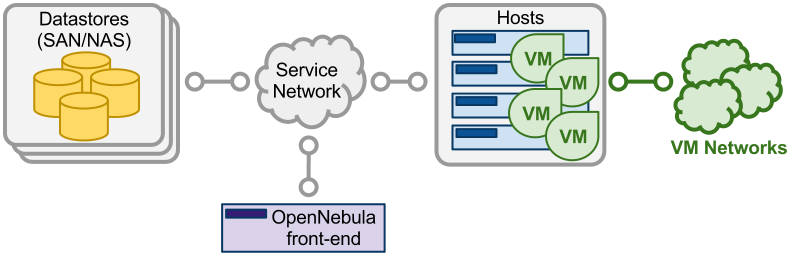
\includegraphics[scale=0.3]{../Bilder/one_high.png}
\caption{Typische OpenNebula Installation}
\label{fig: dasdasdasdas}
\end{figure}
Front-End: Steuert und fuhrt die OpenNebula Dienste aus. �
Schnittstelle fur den Cloud-Administrator. �
Konsolenbasiert oder graphisch (Sunstone Weboberfl�ache).
Hosts: Hosts mit installierter Hypervisor-Software.
Stellen die Ressourcen fur die Ausf � uhrung von virtuellen �
Maschinen.
Aktuell wird Xen, KVM und VMware als Hypervisor
unterstutzt, auch im Mischbetrieb. �
Datastores: Stellen die Basisimages (Betriebssysteminstallation,
Speicherplatz) der virtuellen Maschinen.
%Link: http://www.fbi.h-da.de/~a.schuette/Vorlesungen/Cloud-Computing/Skript/3_Cloud-Infrastrukturen/3_Cloud-Infrastrukturen.pdf
\end{comment}

\chapter{Softwareentwurf}
Nach \cite{Balzert201109} ist der Softwareentwurf die Entwicklung einer software-technischen L�sung im Sinne einer Softwarearchitektur auf Basis der gegebenen Anforderungen an ein Softwareprodukt. 
Die Kunst bei einem Softwareentwurf besteht entsprechend darin, eine Softwarearchitektur zu entwerfen, die die zuvor erarbeiteten funktionalen (Kapitel \ref{sec:FunktionaleAnforderungen}) und nichtfunktionalen Anforderungen (Kapitel \ref{sec:NFA}) betrachtet, einschliesslich der Ber�cksichtigung von Einflussfaktoren wie definierte Randbedingungen. (Kaptitel \ref{sec:Randbedingungen}).
Der Softwareentwurf ist als Richtlinie zu sehen, der bei der Umsetzung der angeforderten Software unterst�tzt.
Die zu erstellende Softwarearchitektur hingegen beschreibt Architekturbausteine, deren Interaktionen und Beziehungen untereinander sowie ggf. deren Verteilung auf physicher Ebene. Dabei ist die spezifizierung der entsprechenden Schnittstellen der einzelnen Architekturbausteine mit zu beachten. F�r die Visualisierung der Architekturbausteine k�nnen verschiedene Abstufungen von Sichten herangezogen werden.
Die Kontextabgrenzung, Bausteinsicht, Laufzeitsicht und die Verteilungssicht.
\begin{comment}
\begin{enumerate}
\item \textbf{Kontextabgrenzung}
%Die Kontextabgrenzung beschreibt die Einbettung des Systems in seine Umgebung 
%sowie die wesentlichen Teile der umgebenden Infrastruktur.
\item \textbf{Bausteinsicht}
%Die Kontextabgrenzung beschreibt die Einbettung des Systems in seine Umgebung sowie die wesentlichen Teiler der umgebenden Infrastruktur.
\item \textbf{Laufzeitsicht}
\item \textbf{Verteilungssicht}
\end{enumerate}
\end{comment}
\begin{figure}[htbp]
  \centering
  \fbox{
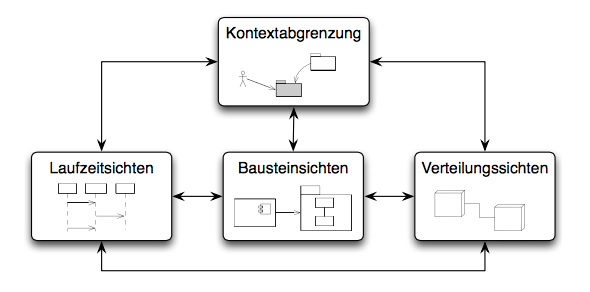
\includegraphics[width=0.9\textwidth]{../Bilder/sichten.png}
  }
  \caption{Vier Arten von Sichten (\cite{Starke201401})}

\end{figure}
\FloatBarrier

\section{Kontextabgrenzung}
Die Kontextabgrenzung beschreibt die Einbettung des Systems in seine Umgebung sowie die wesentlichen Teile der umgebenden Infrastruktur.
Die ermittelten Anforderungen aus Kapitel \ref{sec:FunktionaleAnforderungen} und \ref{NFA} haben ergeben, dass die Hauptfunktionalit�ten aus erstellen, exportieren, importieren, teilen und dem Provisioning von virtuellen Maschinen bestehen.
Um dies weiter zu b�ndeln, k�nnen Teile der Hauptfunktionali�ten von bestimmten Produkten �bernommen werden, die in Kapitel \ref{ch:Evaluation} betrachtet wurden.
VirtualBox kann das Erstellen, Exportieren und den Import von virtuellen Maschinen �bernehmen. Das Konfigurationsmanagement-Systeme Ansible ist darauf ausgelegt, mit bekannten Virtualisierungsl�sungen zusammen arbeiten zu k�nnen und �bernimmt somit die gew�nschten Anforderung nach automatisierter Softwareinstallation. 
Um die beiden Anwendungen zu vereinen, wird als Wrapper Vagrant eingesetzt, das zus�tzliche Funktionen, wie das Teilen (sharen) einer Maschine, mitbringt.
Der Kern der Anwendung ist als eine weitere Schicht anzusehen, der die drei Softwareprodukte weiter vereint und dem Anwender eine entsprechende Benutzeroberfl�che zur Verf�gung stellt.
\begin{center}
 \begin{minipage}{\linewidth}
	\centering
	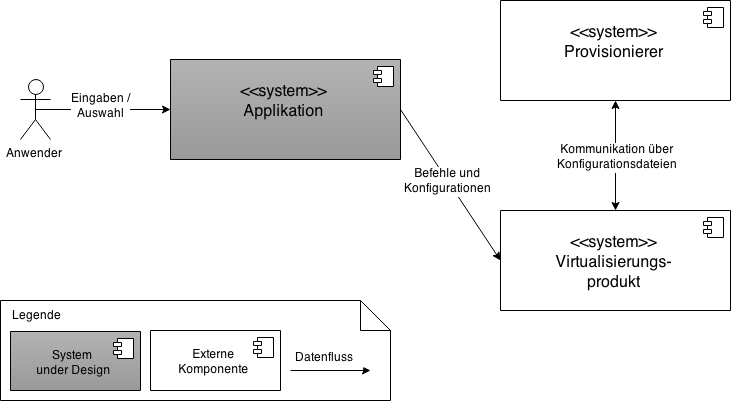
\includegraphics[scale=0.5]{../Bilder/kontextsicht.png}
	\captionof{figure}[kurze Bildunterschrift]{Bildunterschrift}
 \end{minipage}
\end{center}

\subsubsection{Kurzbeschreibung der externen Schnittstellen}
\begin{tabular}{p{4cm} p{10cm}}
\textbf{Eingaben / Auswahl} & Der Anwender t�tigt Eingaben und w�hlt unter Optionen aus, die von der Anwendung bereitgestellt werden. Diese werden direkt von der Applikation verarbeitet\\
 &  \\
\textbf{Befehle und Konfigurationen} & Die Applikation erstellt n�tige Konfigurationsdateien f�r Vagrant und Ansible und leitet Befehle f�r die Weiterverarbeitung an Vagrant weiter\\
 &  \\
\textbf{Kommunikation �ber Konfigurationsdateien} & Vagrant ruft �ber die erstellten Konfigurationsdateien den Konfigurationsmanager Ansible auf, um die virtuelle Maschine in den beschriebenen Zustand zu �berf�hren\\
 & 
\end{tabular}

Die Applikation selbst, inklusive der oben genannten Produkte, l�uft auf einem Server, der zentralisiert positioniert ist und entsprechend angesprochen werden kann.
Der Anwender bekommt von der Applikation eine Weboberfl�che angeboten, die es erm�glicht Eingaben zu t�tigen und Optionen auszuw�hlen, um eine virtuelle Maschine zu erstellen oder zu verwalten.
Um die Applikation auf dem Server zu betreiben, muss eine Internetverbindung bestehen, die Vagrant erm�glicht, das gew�nschte Abbild des Betriebssystems herunterzuladen und die virtuelle Maschine mit anderen Anwendern teilen zu k�nnen.
Die vom Anwender gestellten Anfragen an den VM-Builder, werden in Konfigurationsdateien �bersetzt, die passend f�r Vagrant und Ansible erstellt werden.
Diese Konfigurationsdateien dienen nicht nur zur Erstellung der gew�nschten Applikation, sondern auch zur Kommunikation zwischen Vagrant und Ansible.
Vagrant entnimmt den Konfigurationen das gew�nschte Image, leitet den entsprechenden Download einleitet Vagrant den Download des gew�nschten Images und erstellt mit Hilfe von VirtualBox und ggf Ansible, die zu erwartende virtuelle Maschine. Bei der Erstellung, kommuniziert Vagrant mit Ansible um die vom Anwender zuvor erstellte Zustandsbeschreibung umzusetzen.

\section{Client-Server-Modell}
Das Client-Server-Modell verdeutlicht die Aufgabenverteilung innerhalb einer Applikation und dem Bed�rfnis Prozessorenleistung und gemeinsame Dienste zu zentralisieren.  (\cite{Schaefer200912})\newline
Um eine einigerma�en klare Unterscheidung zwischen Client- und Servert�tigkeiten zu erhalten, kann auf einen geschichteten Architekturstil zur�ckgegriffen werden, der die Aufgaben in folgende Schichten unterteilt:
\begin{enumerate}
\item Benutzerschnittstelle\newline
Die Benutzerschnittstelle enth�lt alles Erforderlich, um direkt mit dem Anwender zu interagieren
\item Verarbeitungsebene\newline
Enth�lt die Anwendung / Kernfunktionalit�t
\item Datenebene\newline
Daten werden unabh�ngig von der Applikation persistent gespeichert
\end{enumerate}
Im Zusammenhang mit dem Client-Server-Modell steht das n-Tier Modell, oder auch Schichtenmodell. Eine Schicht ist entweder ein physikalischer Rechner oder mindestens ein Systemprozess, der eine gewisse Aufgabe �bernimmt. Die einfachste Anordnung dieser Schichten besteht darin, sie auf zwei Computer zu verteilen (2-Tier Modell). Den Client und den Server. Dabei k�nnen die Schichten wie in Abbildung \ref{fig:Client-Server-Anordnungen}  zwischen Client und Server verteilt sein.(\cite{TanenbaumSteen200711})
\begin{figure}[htbp]
  \centering
  \fbox{
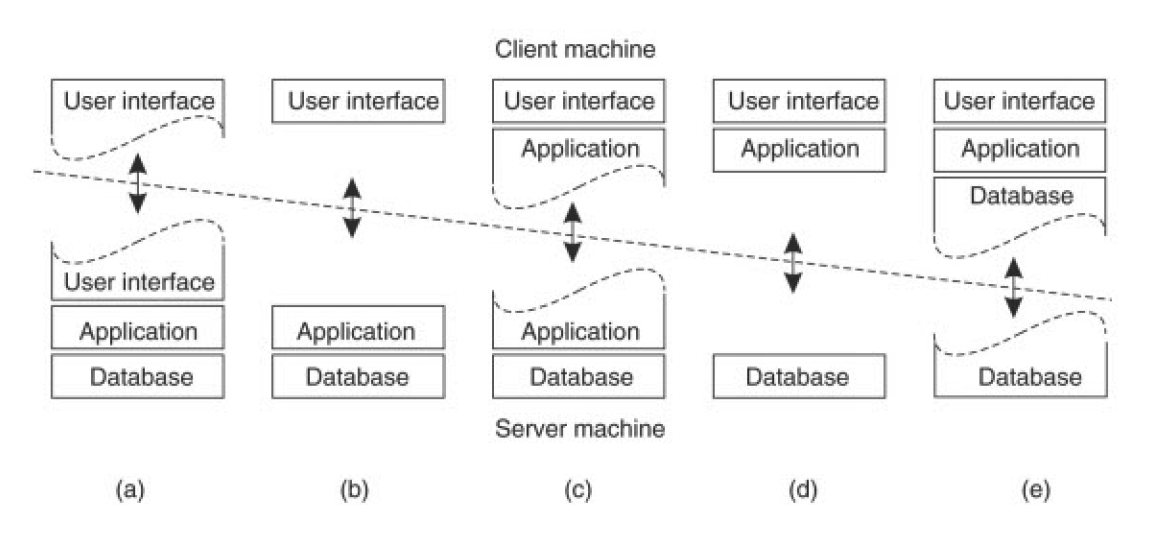
\includegraphics[width=0.9\textwidth]{../Bilder/client-server-anordnungen.png}
  }
  \caption{Client-Server-Anordnungen (\cite{TanenbaumSteen200711})}
	\label{fig:Client-Server-Anordnungen}
\end{figure}
\FloatBarrier
Die in Abbildung \ref{fig:Client-Server-Anordnungen}(a) bis (c) dargestellten Varianten geh�ren zu der Kategorie Thin Clients, die f�r den zu entwickelnden 'VM Builder' im Fokus stehen.\newline
Der Vorteil von Thin Clients ist, dass weniger Client-Software auf die Seite des Anwenders gebracht werden muss. Denn Software auf Clientseite ist nicht nur schwerer zu administrieren, sondern auch f�r Fehler anf�lliger (\cite{TanenbaumSteen200711}).
Die hier angestrebte Client-Server-Anordnung ist die in Abbildung \ref{fig:Client-Server-Anordnungen}(b) gezeigte Variante. Der Client soll so schlank wie m�glich gehalten werden, um dem Anwender einen schnellen Seitenaufbau zu erm�glichen und um lokale Installationen zu verhindern.
Variante (a) w�rde nur dann zum Einsatz kommen, wenn eine entfernte Steuerung der Darstellung gew�nscht w�re, was hier nicht der Fall ist. F�r den Client-Server Aufbau mit Variante (b) geht man davon aus, dass Programmlogik mit zum Client �bertragen wird. Also z.B. eine Eingabe�berpr�fung direkte im Frontend. Da in der Anforderungsanalyse Kapitel \ref{subsec:TechnischeRandbedingungen} festgelegt wurde, dass mit Ruby inkl. des Frameworks Sinatra gearbeitet werden soll, wird die Logik auf der Serverseite implementiert und ben�tigt keinen Anteil auf Client-Seite.

\section{Kommunikation}

\section{Verteilungssicht}




\section{Bausteinsicht}
\section{Laufzeitsicht}

\section{Zusammenfassung}

\chapter{Realisierung}
Dieses Kapitel wird die Umsetzung und die damit verbundene Realisierung des VM-Builders beschreiben. Die Umsetzung geschieht unter der Beachtung der zuvor durchgef�hrten Planung aus Kapitel \ref{ch:Anforderungsanalyse} und der damit verbundenen Integration von Dritt-Anwendungen. Ein wichtiger Aspekt des Kapitels ist die Verdeutlichung von Unterschieden, die zwischen Planung und der Umsetzung auftreten. Die Realisierung selbst wird in erster Linie ein Prototyp des VM-Builders anstreben, wobei auch seine Implementierung sich ganz nach dem Entwurf richtet, der in Kapitel \ref{ch:Entwurf} entstanden ist. Um die Anforderungen aus dem technischen Randbedingungen (Abschnitt \ref{subsec:TechnischeRandbedingungen}) zu erf�llen, geschieht die Umsetzung der Applikation in einer Kombination aus dem Framework Sinatra und Ruby und wird in der IDE 'RubyMine' entwickelt.\newline
Die Realisierung wird in drei Schritte unterteilt:
\begin{enumerate}
\item Aufbau des Servers (Abschnitt \ref{ssec:ServerRealisierung})
\item Installation und Beschreibung der Fremdsoftware (Abschnitt \ref{ssec:SoftwareRealisierung})
\item Erstellung und Implementierung des VM-Builders (Abhschnitt \ref{ssec:SoftwareRealisierung})
\end{enumerate}
Die drei Schritte beinhalten nicht nur Details zu ihrer Umsetzung, sondern auch die Unterschiede zum Entwurf.

\section{Server Realisierung}\label{ssec:ServerRealisierung}
Um die Vorraussetzungen f�r die Entwicklung des VM-Builders zu schaffen, wird der erste Schritt der Aufbauphase angegangen und eine Entwicklungsplatform vorbereitet. Anstelle eines Hardware-Servers, wird zun�chst auf einer virtuelle Maschine entwickelt. Wie bereits in der Einleitung erw�hnt, handelt es sich bei der Entwicklung um einen Prototypen der Applikation und genau auf diesem Aspekt aufbauend, ist eine virtuelle Umgebung zum entwickeln und testen mehr als geeignet.\newline
Zeitgleich wird eine identische Umgebung auf einem VM-Host der HAW aufgebaut, um sp�ter Unterschiede in der Aufbaugeschwindigkeit der virtuellen Maschinen messen zu k�nnen. Einfacherhalber wird in den folgenden Abschnitten lediglich ein Server betrachtet, damit keine Unklarheiten auftreten. Die Unterschiede der Server sind nur rein technischer Natur und unterscheiden sich weder in Applikationsversionen, noch im Aufbau.\newline
Der lokale virtuelle Server wird mit 4GB Arbeitsspreicher, 20 GB Festplattenkapazit�t und Ubuntu 14.04.2 umgesetzt. Der Server auf HAW-Seite, wird mit 16 GB Arbeitsspeicher ausgestattet und einem schnelleren Prozessor. Das Betriebssystem ist ebenfalls Ubuntu 14.04.2.

\section{Fremdsoftware}\label{ssec:SoftwareRealisierung}
Eines der Ergebnisse des Entwurfs war die Verwendung von Fremdsoftware, wodurch gewisse Teile des Funktionsspektrums �bernommen werden sollen. Der zweite Schritt der Realisierung wird sich mit den einzelnen Softwareelementen besch�ftigt, die f�r den Betrieb des VM-Builders eingesetzt werden sollen. In der Evaluation aus Kapitel \ref{ch:Evaluation} sind die ersten Annahmen getroffen worden welche Softwarekomponente sich f�r bestimmte Aufgabenbereiche eignen k�nnten, um sie dann in der in der Verteilungssicht (Abschnitt \ref{sec:Verteilungssicht}) provisorisch zu integrieren. Vorteile der verwendeten Applikationen sind ihre OpenSource Eigenschaften und der damit verbundene Verzicht auf weitere Kosten oder Investitionen. Die einzelnen Applikationen werden noch einmal kurz vorgestell, wobei auf Installationsdetails verzichtet wird.

\subsection{Webserver}
F�r die Pr�sentation des Webinterfaces und f�r die Kommunikation zwischen Client und Server, wird auf den frei erh�ltlichen Apache Webserver, in der Version 2.4.7 zur�ckgegriffen.\newline
Es bietet sich an, einen etablierten Webserver zu nutzen, gerade wenn er den geforderten Open-Source-Aspekt erf�llt. Zudem besitzt Apache einen Marktanteil von 50,51\% an aktiven Webseiten (\cite{Statista:2015:Online}), wodurch das Argument der Etablierung weiter untermauert wird. Durch diesen Faktor kann zudem davon ausgegangen werden, dass die Weiterentwicklung weiter anh�lt, sowie Supportm�glichkeiten auch noch zuk�nftig vorhanden sein werden.

\subsection{Phusion Passenger}
Im Zuge der Vorbereitung auf die Appikation, wird auf Phusions Passenger zur�ckgegriffen, das als ein Modul f�r Apache konzipiert wurde. Phusions Passenger wird prim�r bei Ruby-Applikationen verwendet, um Ruby-Web-Applikationen bereitzustellen. Zudem erleichtert Passenger die Administration von Web-Applikationen und ist essenziel f�r den Betrieb des VM-Builders.\newline

\subsection{VirtualBox}
Ein eigener Entwurf und deren Ausf�hrung einer Virtualisierungsstrategie, w�re weder zielf�hrend noch praktikabel. Deshalb wurde in der Evaluation (Kapitel \ref{ssec:VirtualBox}) eine Analyse der frei zug�nglichen Virtualisierer durchgef�hrt, wodurch letztendlich das Ergebnis VirtualBox als geeigneten Kandidaten herausstellte.
VirtualBox �bernimmt beim VM-Builder die Funktion der Maschinenvirtualisierung und somit den automatisierten Aufbau der Umgebung.

\subsection{Ansible}
Damit die erstellte Umgebung mit Software best�ckt werden kann, wird diese Aufgabe Ansible �bertragen. Ansible kann die gew�nschte Zustandsbeschreibung des Anwenders, direkt auf der virtuellen Maschine umsetzen, ohne dort einen extra Client installieren installieren zu m�ssen. Dies erleichtert nicht nur die Arbeit mit Ansible, sondern erleichtert zudem die Integration von Ansible in den VM-Builder. 

\subsection{Vagrant}
Vagrant dient als Wrapper f�r VirtualBox und Ansible. Die Flexibilit�t von Vagrant erm�glicht das leichte Zusammenspiel der drei Softwarekomponenten. Da Vagrant mit anderen Provisionierern und Virtualisierern zusammenarbeiten kann, ist ein Austausch von Ansible und VirtualBox in einem begrenzen Zeitrahmen m�glich.\newline
Der VM-Builder wird �ber Befehlsaufrufe direkt mit Vagrant kommunizieren und durch entsprechende Befehle den Aufbau, die Deaktivierung, das Sharing usw. ausl�sen.

\subsection{Bundler}
Um in Ruby-Pojekten Abh�ngigkeiten zu genutzen Paketen zu verwalten und ggf. deren Versionen zu spezifizieren, kann auf Bundler zur�ckgegriffen werden.
Durch Bundler k�nnen einheitliche Umgebungen f�r Projekte geschaffen und der Wiederaufbau der gleichen Umgebung beschleunigt werden. Durch seine Eigenschaft, Ruby-Komponenten sofort und automatisch installieren zu k�nnen, ist Bundler pr�destiniert f�r die Umsetzung einer automatisierte Installation des VM-Builders.

\subsection{Datenbank}
Um die objektorientierte Welt mit der Relationalen Welt der Datenbanken in Einklang zu bringen, k�nnen OR-Mapper helfen. Durch ihre �bersetzung von Quellcode, k�nnen programmatisch Tabellenkonstrukte erzeugt und Beziehungen zwischen den gew�nschten Tabellen definiert werden. Datamapper ist eines der Beiden popul�rsten ORM Frameworks f�r Ruby und wird die beschriebenen Aufgaben im VM-Builder �bernehmen.\newline
Ein Beispiel f�r die Funktionsweise von Datamapper, ist die Definition der Tabelle Machine, die aus vier Attributen besteht inklusive ihrer Typ-Eigenschaften, sowie ihrer Relation zu anderen Tabellen.
\begin{lstlisting} [caption={ORM Framework Datamapper},label={code:ORMTable}, language=Ruby]
class Machine
  include DataMapper::Resource

  property :id, Serial 
  property :name, String, :length => 255, :required => true 
  property :ip, String, :length => 15
  property :description, String, :length => 255
  property :status, Integer 

  has n, :files
  has n, :machinesoftwares
  has n, :softwares, :through => :machinesoftwares
  belongs_to :vmimage
end
 \end{lstlisting}
Programmatischer Zugriff auf die Tabellen kann �ber SQL-Befehle bereitgestellt werden, oder �ber typischerweise vorhandenen Befehle des ORM-Frameworks.
Um z.B aus der Tabelle \textbf{Machine} alle Daten einmal abzurufen gen�gt der Befehl 'Machine.all'. 
\begin{lstlisting} [caption={ORM Framework command},label={code:ORMCommand}, language=Ruby]
 def all_machines?
    Machine.all
  end
\end{lstlisting}

\section{Implementierung}\label{ssec:Implementierung}
Nach dem Aufbau der Server und der Installation der ben�tigten Softwarekomponenten, steht im n�chsten Abschnitt die Implementierung des Protoypen im Vordergrund.
Ziel des Prototypen ist grundlegende Funktionen zu implementieren und zu testen, in wie weit sie durch die Anforderung realisierbar sind.\newline
Entsprechend stehen folgende Funktionalit�ten im Mittelpunkt:
\begin{enumerate}
\item[\textbullet] Automatisierter Aufbau einer virtuellen Maschine 
\item[\textbullet] Provisionierung
\item[\textbullet] Speichern von VM-Konfigurationen
\item[\textbullet] Softwarebundles erstellen
\item[\textbullet] Virtuelle Maschine 'sharen'
\end{enumerate}
Zuvor wird ein Blick auf strukturellen Ans�tze der Entwicklung geworfen, in dem allgemein auf die Komponenten-Umsetzung eingegangen wird und auf entsprechende �nderungen.
\subsection{Komponenten Umsetzung}
Wie bereits in der Einleitung des Kapitels erw�hnt, wird der 'VM-Builder' mit Ruby inklusive dem Framework Sinatra umgesetzt. Um dem MVC-Konzept zu entsprechen, werden die definierten Komponenten aus \ref{ssec:Bausteinsicht} in der folgenden exemplarischen Ordner-/Dateistruktur (\ref{code:Filestructure}) umgesetzt.
\begin{lstlisting} [caption={Exemplarische Ordnerstruktur VM-Builder},label={code:Filestructure}, language=Ruby]
config.ru
app.rb
helpers/
  persistence_handler.rb
models/
  init.rb
routes/
  init_controller.rb
views/
  init_view.erb
\end{lstlisting}
Controller und Views aus der der Benutzerschnittstelle werden in den Ordnern 'routes' und 'views' erstellt. Bestandteile aus der Verarbeitungsebene und Datenebene werden in 'models' und 'helpers' gespeichert.\newline
Da Ruby/Sinatra zul�sst auf Klassen zu verzichten, sind die Controller als organisatorische Einheit konzepiert mit der entsprechenden Logik in den verwendeten Modellen.
\begin{lstlisting} [caption={Controller Beispiel},label={code:ControllerExample}, language=Ruby]
require './models/administration_manager'
require_relative 'softwareadmin_controller'

get '/log' do
  @content = admin_mgr.log_content?
  erb :logfile
end

put '/log' do
  admin_mgr.update_log_config(params['logpath'])
  admin_mgr.create_logfile(params['logpath'])
  redirect '/admin'
end
\end{lstlisting}
W�hrend die Views in HTML geschrieben und Helper, sowie Models als Ruby-Klassen definiert sind.\newline
Durch die Umsetzung haben sich Unterschiede bez�glich des Entwurfs herausgestellt, die folgende Bausteinsicht ergeben haben. 
\begin{figure}[htb]
  \centering
\includegraphics[width=0.9\textwidth]{../Bilder/Bausteinsicht_Impl.png}
  \caption{Bausteinsicht Level 1}
	\label{fig:Bausteinsicht_MVC_Umsetzung}
\end{figure}
\FloatBarrier
Abgesehen von der Entstehung neuen Beziehungen zwischen Komponenten, ist eine der wesentlichen �nderungen das Wegfallen des ConfigurationfileHandlers. Seine Aufgabe bestand im Lesen und Beschreiben einer Konfigurationsdatei, die Konfigurationen des gesamten 'VM-Builders' beinhalten sollte. 
Anstelle der Konfigurationsdatei, werden die Konfigurationen in der Datenbank gepflegt.
Die daraus entstehenden Vorteile sind eine zentrale Steuerung f�r den persistenten Speicher und �nderungen, sowie das Hinzuf�gen von neuen Konfiguration sind deutlich vereinfacht worden.

\subsection{Datenbank}
Wie bereits erw�hnt, wird im Gegensatz zur Planung, ein Tabellenkonstrukt angewendet, um Konfigurationen zu persistieren. Dies spart zu erstellende Komponenten und zentralisiert den Zugriff und die Datenhaltung.
Zur Umsetzung von Konfigurationstabellen werden in der Regel zwei Konzepte vorgeschlagen:
\begin{enumerate}

\item \textbf{Name-Value-Pair Table}\newline
Name-Value Pair Tabellen bestehen nur aus zwei Spalten. Eine f�r den Konfigurations-Typen und die Andere f�r den zugeh�rigen Wert. Kommen neue Konfigurationen dazu, werden die einfach an die Tabelle angehangen.
\begin{lstlisting} [caption={Name-Value-Pair Table},label={code:Name-Value-PairTable}]
  ConfigOption   |   Value
-----------------+-------------
 CompanyName     | ACME Inc.
 StartFullScreen | true (or 1, or Y, ...)
 RefreshSeconds  | 20
 ...             | ...
\end{lstlisting}


\textbf{Vorteil}
\begin{enumerate}

\item Neue Konfigurationen ben�tigen keine Rekonfiguration des Tabellenschemas
\item Schlanke Tabellenstruktur. Neue Konfigurationen werden einfach angehangen\newline
\end{enumerate}

\textbf{Nachteil}
\begin{enumerate}
\item Jede Konfiguration hat den gleichen Typ
\item Alles wird als String/Varchar gespeichert
\item F�r die Arbeit mit den Werten der Konfigurationstabelle, sollte bekannt sein, welcher Typ sich eigentlich hinter dem Wert verbirgt
\end{enumerate}

\item \textbf{Single-Row Table}\newline
Bei Single-Row Tabellen wird die Struktur gedreht. Jede Konfiguration besteht aus einer eigenen Spalte. Die darunter liegende Zeile beinhaltet die Werte.
\begin{lstlisting} [caption={Single-Row Table},label={code:Single-RowTable}]

CompanyName | StartFullScreen | RefreshSeconds | ...
------------+-----------------+----------------+-----
  ACME Inc. |      true       |       20       |  ...
\end{lstlisting}

\textbf{Vorteil}
\begin{enumerate}
\item Jede Spalte hat bekommt den entsprechenden Datentyp
\item Durch den exakt angegebenen Typ jeder Spalte, kann in der Programmierung besser mit den Werten umgegangen werden
\item Jeder Spalte k�nnen leichter Standardwerte zugeordnet werden\newline
\end{enumerate}

\textbf{Nachteil}
\begin{enumerate}
\item Das Tabellenschema muss ge�ndert werden, wenn neue Einstellungen hinzugef�gt werden
\item Die Tabelle kann schnell unleserlich werden, wenn zu viele Einstellungen in der Tabelle enthalten sind
\end{enumerate}
\end{enumerate}
In der Umsetzung wurde das Konzept der '\textbf{Name-Value-Pair Table}' verwendet.
Auch wenn dieses Konzept weniger Vorteile als '\textbf{Single-Row}', spricht das leichtere Einpflegen von neuen Konfigurationseigenschaften und die bessere Lesbarkeit, f�r das Konzept.

\subsection{Funktionen}
Die Realisierung aller geplanten Controller, Models und Views hat das Funktionsspektrum der Applikation fast vollst�ndig erf�llt.\newline
So sind folgende Funktionen durch die bisherige Implementierung realisiert worden:
\begin{description}
\item \textbf{Erstellung einer virtuellen Maschine} \\
Die Komponente 'Main-Representation', die die zentrale Steuerung darstellt, kommuniziert kann die BuildingProcess-Komponente aufrufen in der die Darstellung f�r den geleiteten Aufbau einer virtuellen Maschine gehalten wird und die Schnittstelle zu der entsprechenden Logik. Der Aufbauprozess beinhaltet die Benamung der gew�nschten Maschine, Optionen wie IP-Adresse und die Auswahl an Softwarekomonenten. Echtzeitinformation �ber den Aufbauprozess sind nicht implementiert. Allerdings im Logfile nachlesbar.
VagrantControl liefert in Kombination mit dem SystemFileManager die Befehle f�r den Aufbau einer Maschine. Der SystemfFileManager bietet eine Methode f�r direkte Systemaufufe an, mit der VagrantControl Vagrant Befehle absetzen kann.
\item \textbf{Provisioning} \\
Die Provisionierung wurde in den Aufbau mit integriert und wird durch die Komponente MachineConstruction realisiert. Um genauer zu sein, durch die Klasse 'YamlBuilder'.
Die ausgew�hlte Software, wird durch diese Klasse in eine YAML-Datei �bersetzt und mit Einstellungen aus der Konfigurations-Tabelle angereichert.
Beinhaltet die Auswahl an Software Unterkomponenten und/oder Dateien, die auf den Zielhost �bertragen werden sollen, wird die YAML-Datei automatisch entsprechend angepasst.

\item \textbf{VM-Konfigurationen speichern} \\
Sobald eine virtuelle Maschine erfolgreich aufgebaut wurde, Name und optionale Einstellungen der Maschine, sowie ausgew�hlten Softwarekomponenten durch Transaktionen im Datamapper gespeichert. Durch die verwendeten Transaktionen, wird vermieden, dass inkonsistente Konfigurationen gespeichert werden und sichergestellt, dass diese auch nur im Erfolgsfall gesichert werden.\newline
Solange die Maschine durch keinen Anwender gel�scht wird, bleiben die gespeicherten Parameter bestehen.

\item \textbf{Softwarebundles erstellen} \\
Softwarebundles helfen dabei, Software mit Abh�ngigkeiten zu anderen Softwarekomponenten und Dateien zu erstellen und im System zu hinterlegen.
So wird die M�glichkeit geschaffen, Software zu installieren, die mehrere Installationsschritte ben�tigt.
Die SystemAdministration-Komponente h�lt daf�r die entsprechende Implementierung vor. Da die Implementierung organisatorisch zur Administration geh�rt, wurde sie in diesem Paket platziert. Auch hier wird die Speicherung der Einstellungen durch Transaktionen bewerkstelligt, um keine Inkonsistenzen zu verursachen. Dem Anwender wird die M�glichkeit geboten, durch seine Eingaben zu entscheiden, was f�r eine Software gespeichert wird. W�hlt er keine Relationen zu anderen Softwarekomponenten aus und l�sst er die M�glichkeit aus Dateien zu transferieren, wird automatisch nur eine standard Software zur Auswahl hinzugef�gt. Erst durch die Auswahl von Relationen und/oder Dateien, wird es ein Softwarebundle. Die Umsetzung der Auswahl geschieht in dem Model 'SoftwareEditor' der seine Entscheidung an den 'PersistenceHandler' weitergibt.

\item \textbf{VM-Sharing} \\
Das 'Sharing' einer bestehende virtuellen Maschine wird durch die interne Implementierung von Vagrant �bernommen. Die Zust�ndigkeit um die Funktion in den 'VM-Builder' zu �bernehmen und auszul�sen, �bernimmt die Klasse 'VagrantControl'. Wie auch bei dem Aufbau einer virtuellen Maschine, verwendet 'VagrantControl' die Funktion des 'SystemfileManagers' um den entsprechenden Befehl abzusetzen und an Vagrant selber weiterzuleiten. Das Teilen oder 'Sharing' einer virtuellen Maschine wird allerdings durch die Portsperrung des jeweiligen Netzwerkes eingeschr�nkt. Ist der Port 4567 gesperrt, wird durch Vagrant eine Fehlernachricht generiert und das Teilen der Maschine nicht ausgef�hrt. Bei erfolgreichem 'Sharing' wird ein SSH-Share erstellt. Die SSH Variante hat den Vorteil, dass Port und ggf. Passwort optional eingerichtet werden k�nnen, durch Angaben von erweiterten Parametern.
\end{description}



\chapter{Schluss}\label{ch:Schluss}
Der Schluss dieser Arbeit fasst noch einmal alle Kapitel in K�rze zusammen und bildet ein Fazit in Bezug auf das entwickelte Projekt. Der danach folgende Ausblick geht auf Funktionen und Anwendungsgebiete der Applikation ein, die zuk�nftig realisiert werden k�nnen.
\section{Zusammenfassung und Fazit}
Das Ziel dieser Arbeit war die Entwicklung einer Applikation, die einen schnellen und unkomplizierten Aufbau von virtuellen Maschinen erm�glicht sowie deren Verwaltung und einer unkomplizierten Steuerung. Die Applikation sollte dem Anwender erm�glichen, eigenst�ndig dessen virtuellen Aufbauten zu erstellen und zu verwalten.
Die Planung der Applikation (in der Arbeit VM-Builder genannt) erfolgte durch eine detaillierte Anforderungsanalyse in Kapitel \ref{ch:Anforderungsanalyse}. In der Anforderungsanalyse wurden die funktionalen- und nichtfunktionalen Anforderungen eruiert und durch die eigenen Anforderungen an die Applikation erg�nzt. Die daraus entstandenen Use-Cases formten, bezogen auf die Verwendbarkeit, die ersten Details  und stellten die prim�ren Funktionen heraus. Mockups verhalfen den Applikationskontext in eine erste Form zu bringen und Optik, Bedienbarkeit und Funktionen zu verbinden. Die anschlie�ende Evaluation von Open-Source-Anwendungen (Kapitel \ref{ch:Evaluation}) ergab verschiedene Applikationen, die den Funktionsumfang unterst�tzen. Vagrant stellte sich als hervorragender Dritt-Anbieter f�r n�tige Funktionalit�ten heraus. F�r die Zustandsumsetzung auf der gew�nschten Maschine wurde Ansible ausgew�hlt. So wurden etablierte und vorhandene Anwendungen in die Planung integriert, um das Funktionsspektrum zu verbessern.\newline
Der Entwurf in Kapitel \ref{ch:Entwurf} basiert auf der vorhergegangenen Anforderungsanalyse und greift deren Aspekte auf, um die programmatische Umsetzung zu definieren. Im Softwareentwurf wurde erarbeitet, die Applikation nach bestimmten Systemarchitekturen zu gliedern. So wurde das Client-Server-Modell und das MVC-Entwurfsmuster erarbeitet und bei der Konzeptionierung der einzelnen Komponenten ber�cksichtigt. Anschlie�end wurden verschiedene Sichten verwendet, die unterschiedliche Blickwinkel auf die Applikation geben und damit bei der Planung unterst�tzend wirkten. Im Laufe des Entwurfs stellte sich die Kl�rung der Datenbankstruktur als expliziter Punkt heraus, die durch zwei typische Datenbanksichten entworfen wurde. Zuerst wurde das Entity-Relationship-Model (auch als ERM bezeichnet) als Darstellungsform gew�hlt, um Beziehungen und Attribute der Entit�ten darzustellen. Das darauf folgende relationale Datenbank-Modell basiert auf den Ergebnissen des ERMs und bildete einen Entwurf ab der nah an der Umsetzung ist. Relationen zwischen Tabellen wurden dort genauer betrachtet und ggf. nach Regeln der Datenbank-Normalisierung aufgel�st. Das Resultat sind neue Koppeltabellen (Zwischentabellen), die bei der Umsetzung zu ber�cksichtigen sind.\newline
Bei der Umsetzung des VM-Builders in Kapitel \ref{ch:Realisierung} stellten sich teilweise Unterschiede zur Planung heraus. Eine der gr��ten �nderungen betraf den Wegfall der geplanten Konfigurationsdatei. Diese sollte Einstellungen des VM-Builders beinhalten und durch entsprechende Komponenten ausgelesen und beschrieben werden. Konfigurationen werden zuk�nftig in der bereits bestehenden Datenbank verwaltet. So wird der Implementierungsaufwand verringert und nur ein persistenter Speicher verwendet. Die entsprechende Umsetzung der Konfigurationstabellen ist in Abschnitt \ref{ssec:DatenbankImpl} nachzulesen. Die geplante Struktur der Komponenten konnte beibehalten werden, wobei sich teilweise neue Assoziationen zwischen diesen herausstellte, die in der Planung noch nicht ber�cksichtigt wurden.
Die im Entwurf beschriebenen Architekturstile konnten �bernommen werden und halfen bei der Umsetzung. Der komplette Entwurf, beschleunigte nicht nur die Umsetzung, sondern verhalf zu einer �bersichtlichen Strukturierung. Auch die Vorgaben, die Komponenten mit hoher Koh�sion und niedriger Kopplung zu entwerfen, kam der Umsetzung zugute. Alle Komponenten k�nnen leicht ausgetauscht werden und erf�llen den zugedachten Zweck. Die GUI wurde optisch den Mockups angepasst, um den Prototypen �bersichtlich und einfach steuerbar zu machen. Alle geplanten Funktionen des VM-Builders sind im Testumfeld voll funktionsf�hig. Im zweiten Aufbau, der im HAW-Umfeld stattgefunden hat, wurde das Teilen von Maschinen mit anderen Anwendern durch die Netzwerkbeschr�nkungen unterbunden. Komplikationen wie diese lassen sich aber durch konkrete Einstellungen in den verwendeten Softwarekomponenten beheben.

\section{Ausblick}\label{sec:Ausblick}
Bei der Entwicklung und Planung der Applikation sind weitere Ideen und Anwendungszwecke entstanden, die allerdings in der zeitlichen Begrenzung und mit der vorhandenen Arbeitskraft nicht umzusetzen werden konnte. Vorstellbar w�re die Erweiterung des Funktionsumfangs, so dass ganze Infrastrukturen nachgebildet werden k�nnten. Das bedeutet, dass mehrere Server, inklusive deren Softwarebestandteile, nachgebaut werden k�nnten und das mit minimalem Aufwand. Die Basis daf�r bietet der jetzige Entwicklungsstand. Eine entsprechende Erweiterung w�re durch ein umfangreiches Konfigurationsmen� und die Anpassung der Komponenten, die f�r die Kreierung der Konfigurationsdateien n�tig sind, m�glich. Die zugrunde liegenden Softwarekomponenten beinhalten in deren Funktionsumfang die M�glichkeit mehrere Maschinen gleichzeitig zu erstellen und diese unabh�ngig voneinander zu provisionieren. Extras wie unterschiedliche und explizite IP-Adressen zu vergeben ist z.B. eine minimale Konfigurationsangelegenheit. Da Ansible anbietet vorgefertigte Zustandsbeschreibungen (Playbooks) zu verwenden, k�nnten auch zuvor geschriebene Zustandsbeschreibungen nachtr�glich in der zu erstellenden virtuellen Infrastruktur umgesetzt und f�r sp�tere Zwecke abgelegt werden. Zudem w�re eine Erweiterung denkbar, die automatisiert produktionsnahe Umgebungen erstellt und gleichzeitig den aktuellen Datenbestand zur Verf�gung stellt. So h�tten Tester und Entwickler schneller und effektiver einen Abzug des Produktionsumfeldes, um ihren T�tigkeiten besser nachzugehen. Zu beachten w�re bei allen Aufbauten, die Integration der Schnittstellen zwischen den verwendeten Systemen.
\chapter*{Anhang}\label{ch:Anhang}
\addcontentsline{toc}{chapter}{Anhang}

\section*{Aufbau einer virtuellen Maschine}\label{sec:Aufbau}
\textcolor{white}{\textbf{Aufbau einer virtuellen Maschine}}
\begin{figure}[htbp]
  \centering
  \fbox{
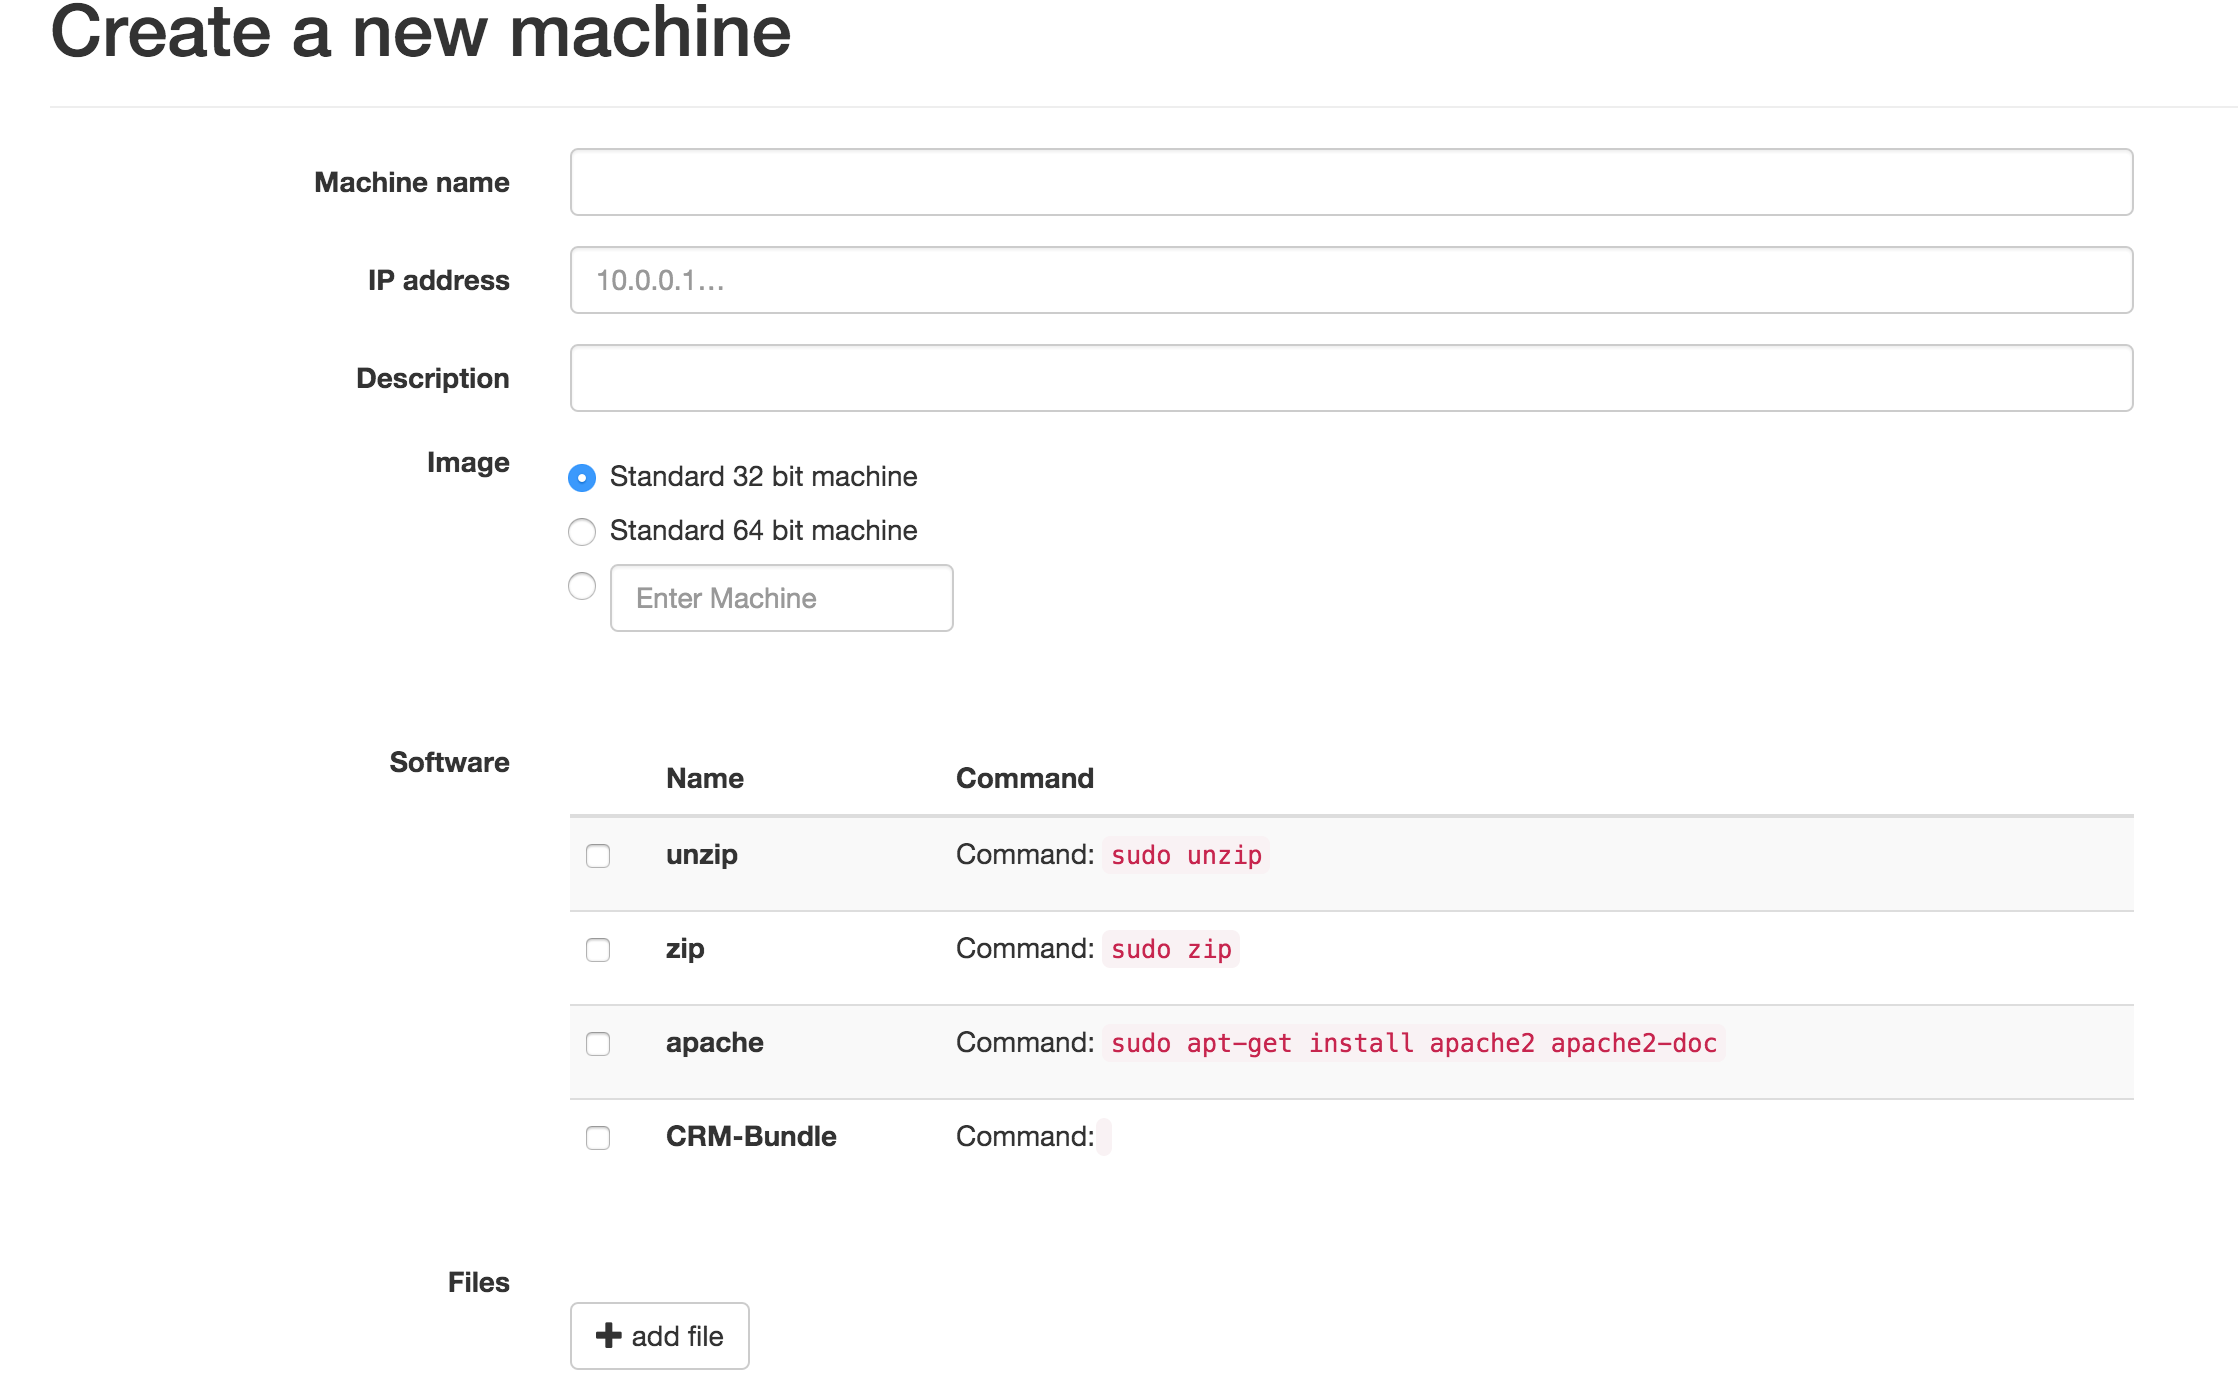
\includegraphics[width=0.9\textwidth]{../Bilder/Anhang/create_machine.png}
  }
  \caption{Men� zum Erstellen einer virtuellen Umgebung}
	\label{fig:create_machine}
\end{figure}
\FloatBarrier
\pagebreak

\section*{Verwaltung der virtuellen Maschinen}\label{sec:Verwaltung}
\textcolor{white}{\textbf{Verwaltung der virtuellen Maschinen}}
\begin{figure}[htbp]
  \centering
  \fbox{
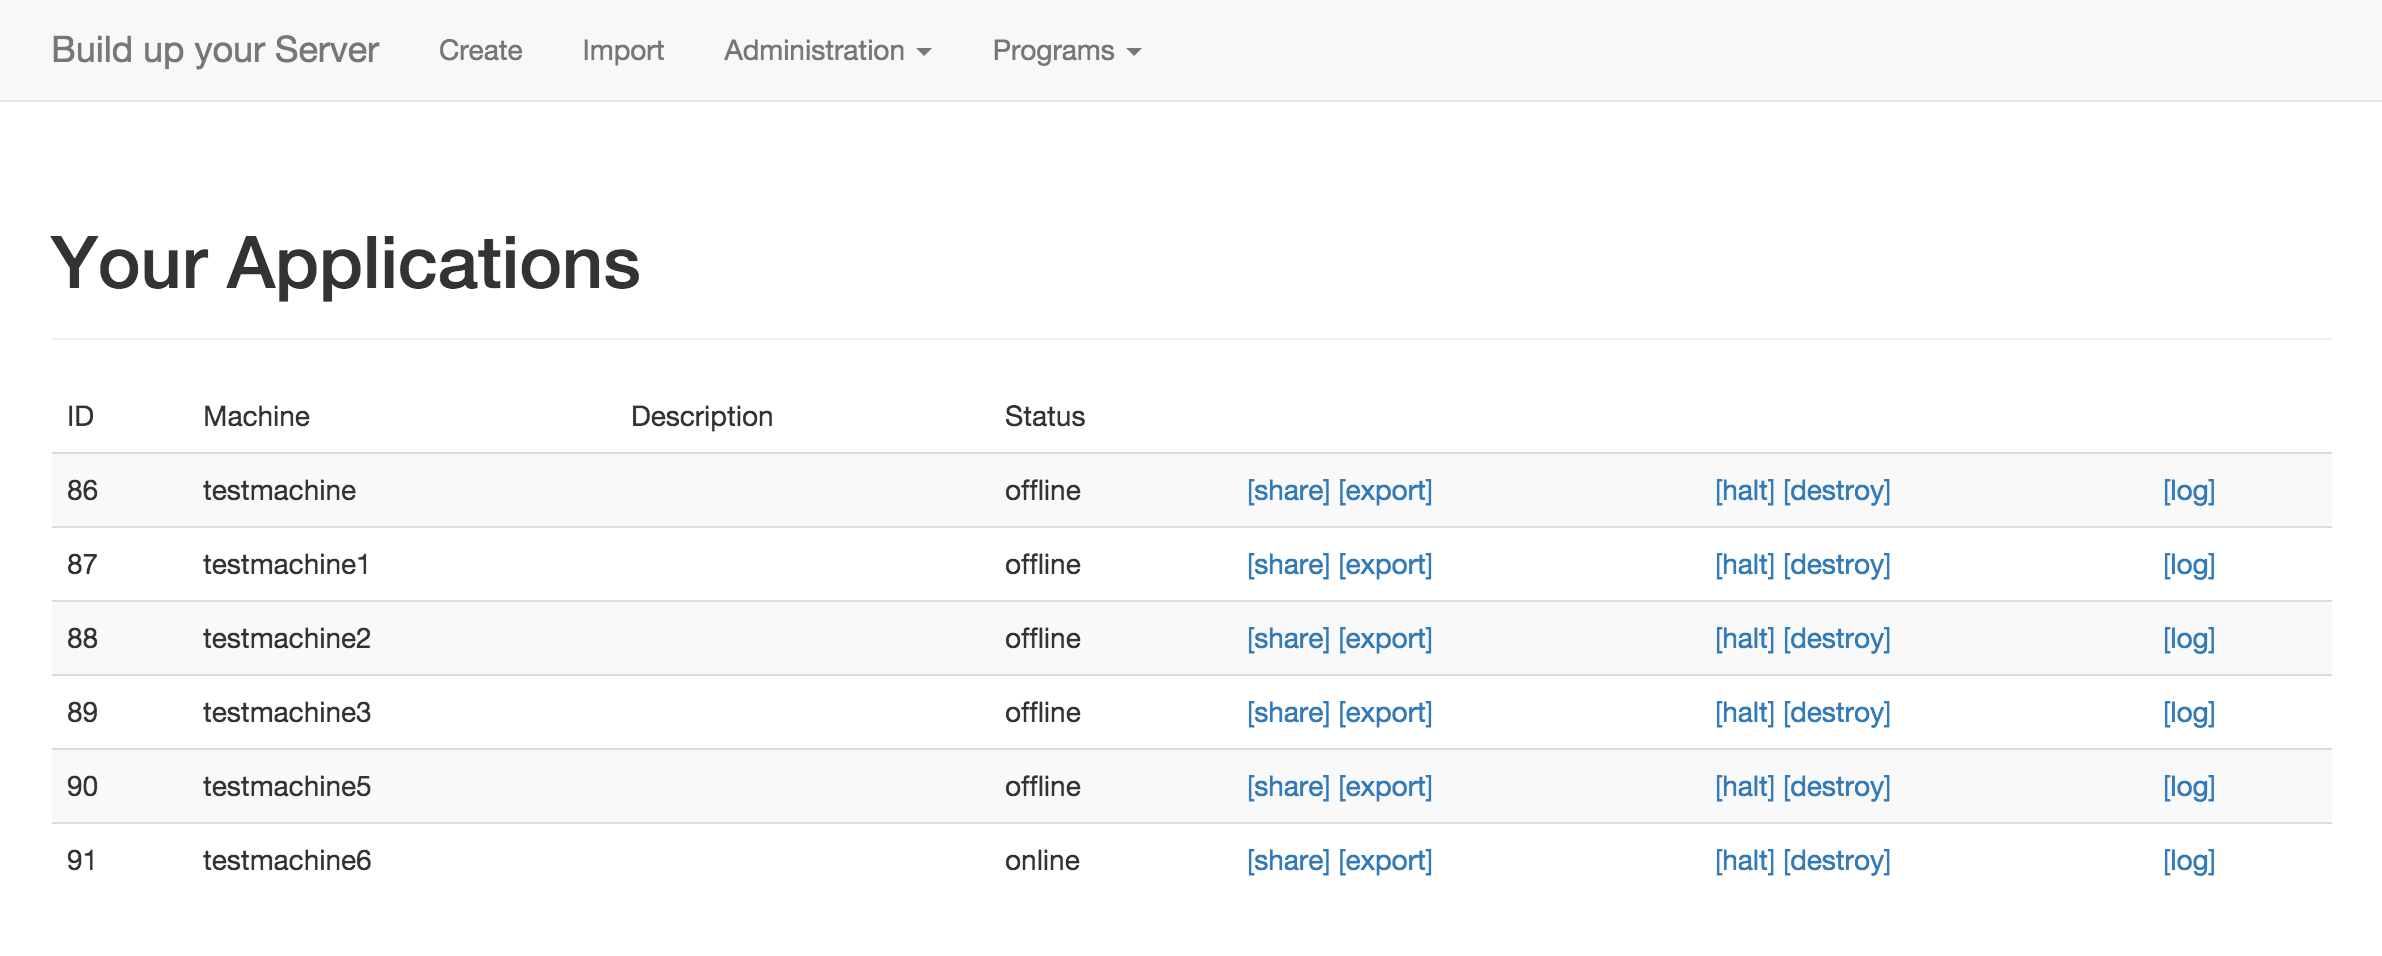
\includegraphics[width=0.9\textwidth]{../Bilder/Anhang/machine_overview.png}
  }
  \caption{�bersicht aller aktuellen virtuellen Maschinen}
	\label{fig:machine_overview}
\end{figure}
\FloatBarrier


\section*{Externer Zugriff}\label{sec:Sharing}
\textcolor{white}{\textbf{Externer Zugriff}}
\begin{figure}[htbp]
  \centering
  \fbox{
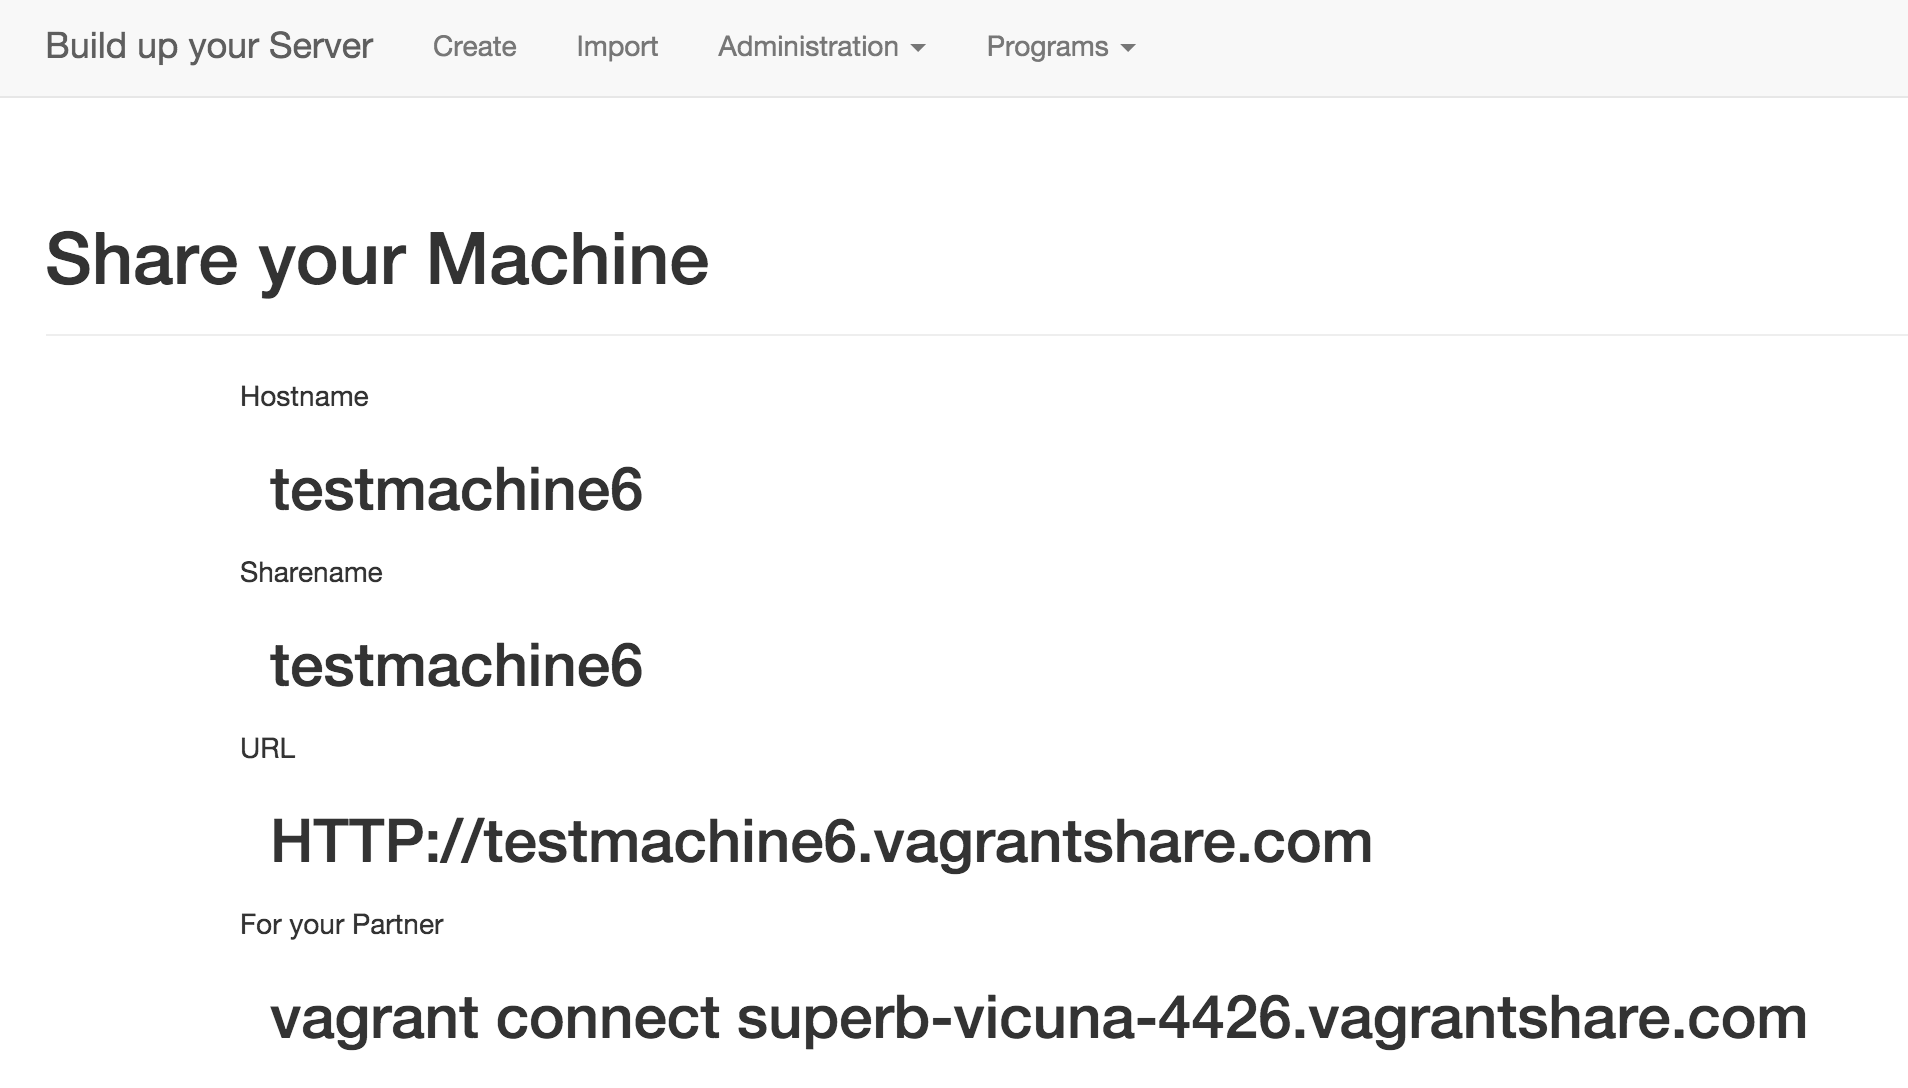
\includegraphics[width=0.9\textwidth]{../Bilder/Anhang/sharing.png}
  }
  \caption{Externe Zugriffsoptionen auf eine virtuelle Maschine }
	\label{fig:share}
\end{figure}
\FloatBarrier

\section*{Import}\label{sec:Import}
\textcolor{white}{\textbf{Import}}
\begin{figure}[htbp]
  \centering
  \fbox{
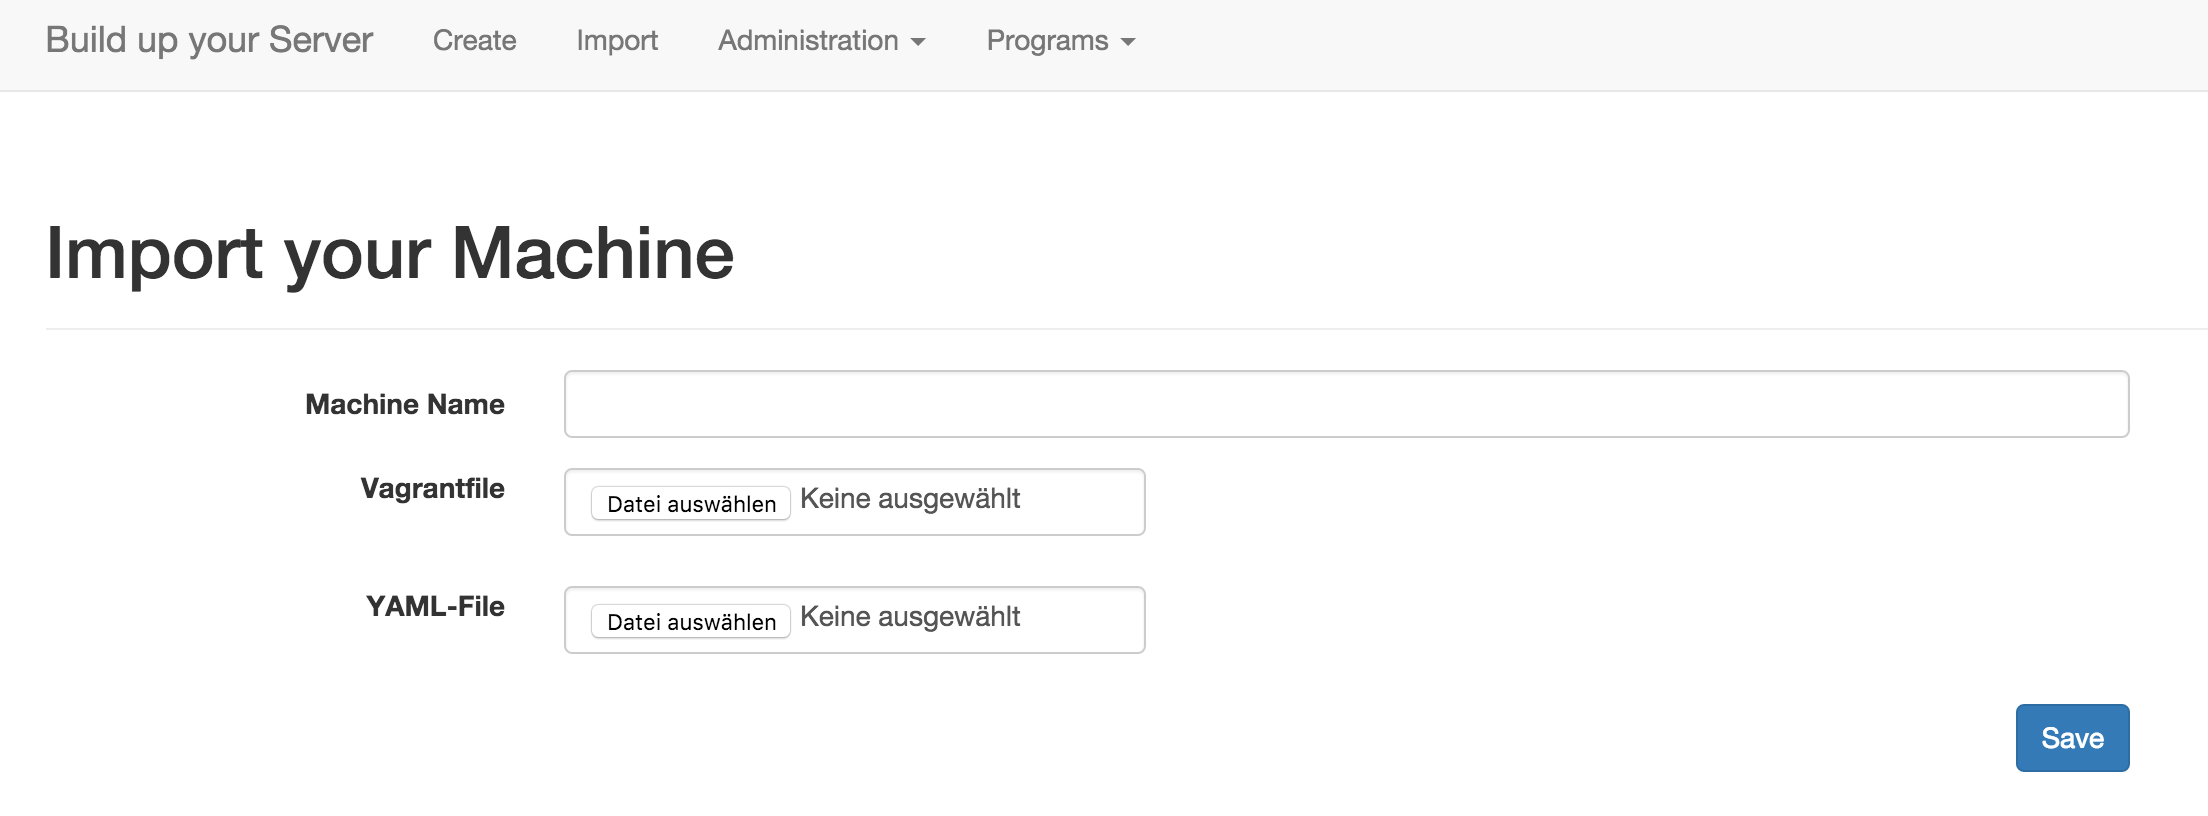
\includegraphics[width=0.9\textwidth]{../Bilder/Anhang/import.png}
  }
  \caption{Import durch Konfigurationsdateien}
	\label{fig:import}
\end{figure}
\FloatBarrier


\section*{Log}\label{sec:Log-Dateien}
\textcolor{white}{\textbf{Log}}
\begin{figure}[htbp]
  \centering
  \fbox{
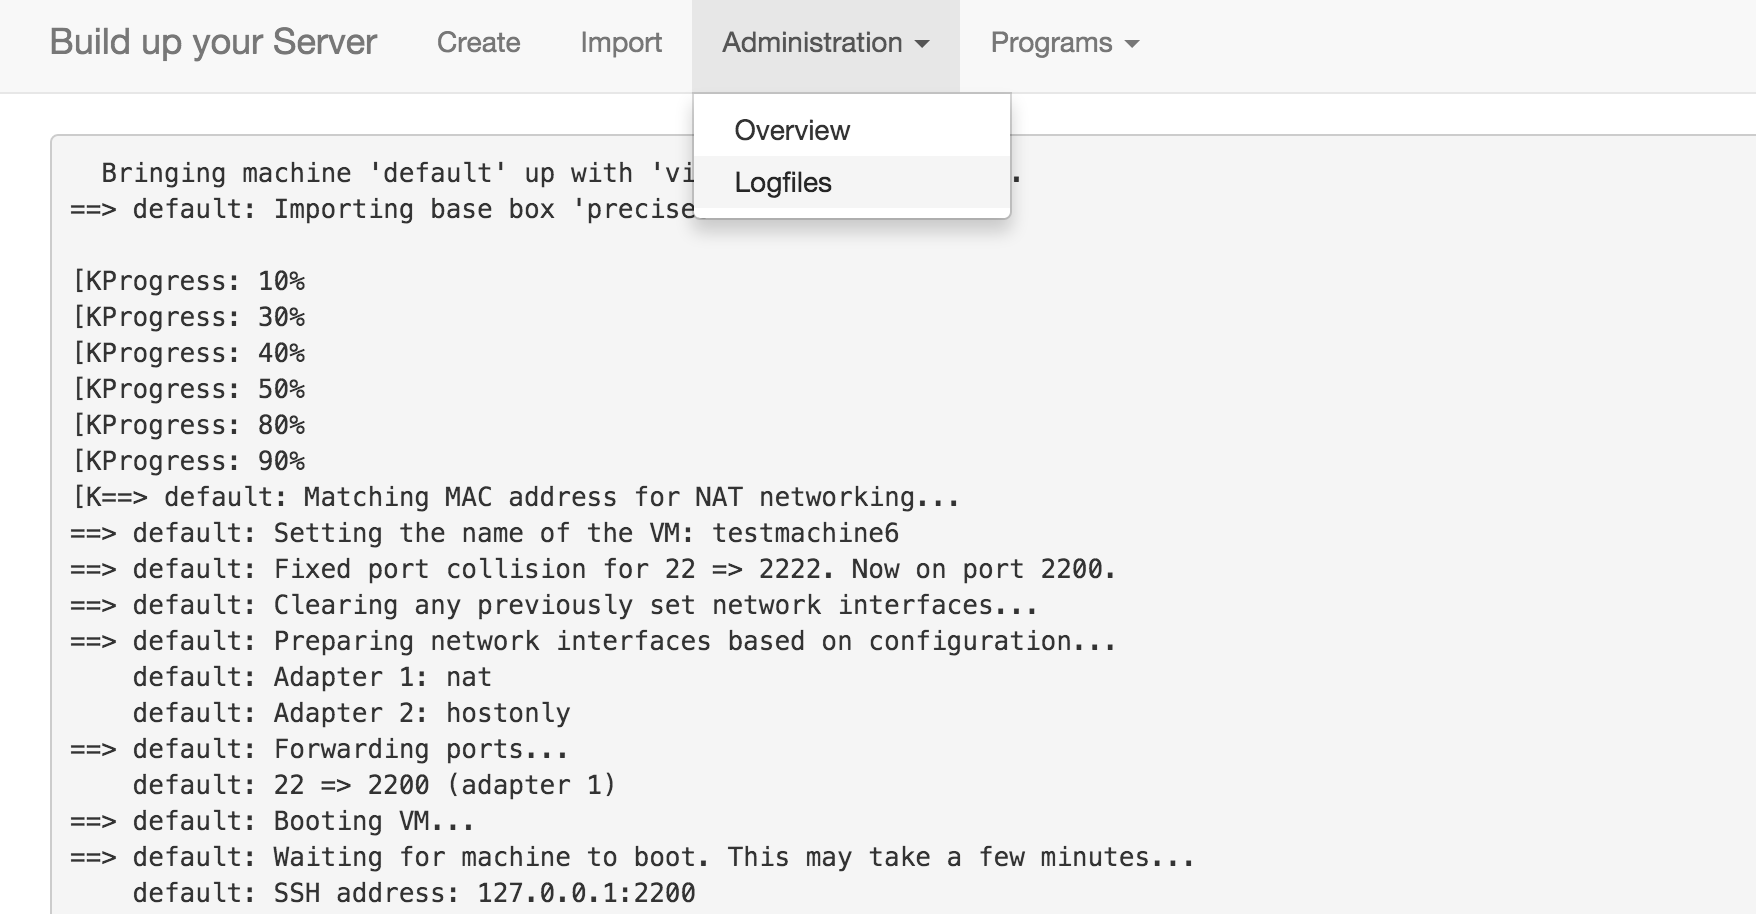
\includegraphics[width=0.9\textwidth]{../Bilder/Anhang/log.png}
  }
  \caption{Allgemeine Logdatei}
	\label{fig:log}
\end{figure}
\FloatBarrier

\section*{Administration}\label{sec:Administration}
\textcolor{white}{\textbf{Administration}}
\begin{figure}[htbp]
  \centering
  \fbox{
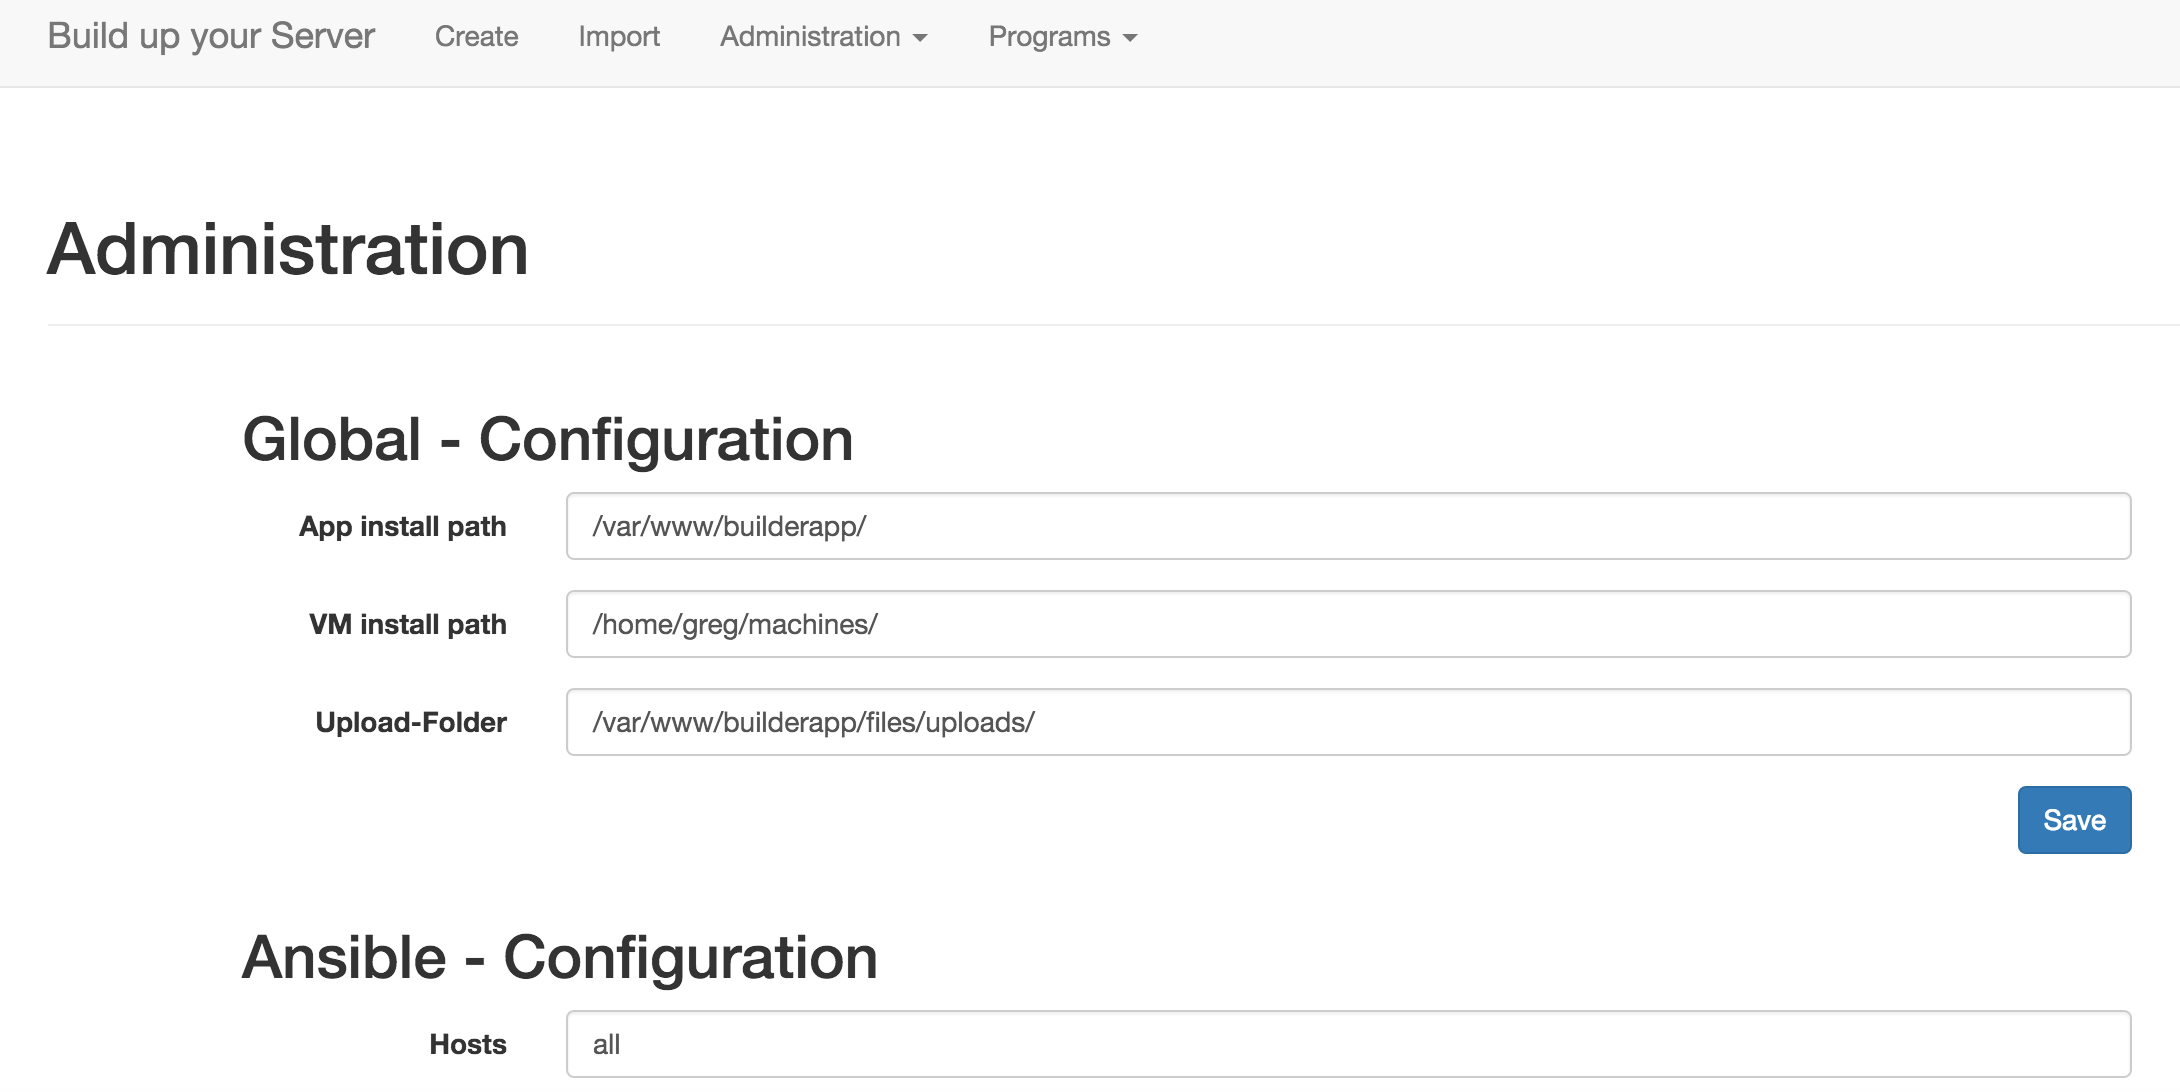
\includegraphics[width=0.9\textwidth]{../Bilder/Anhang/admin_1.png}
  }
  \caption{Administration des VM-Builders (Teil 1)}
	\label{fig:admin1}
\end{figure}
\FloatBarrier

\begin{figure}[htbp]
  \centering
  \fbox{
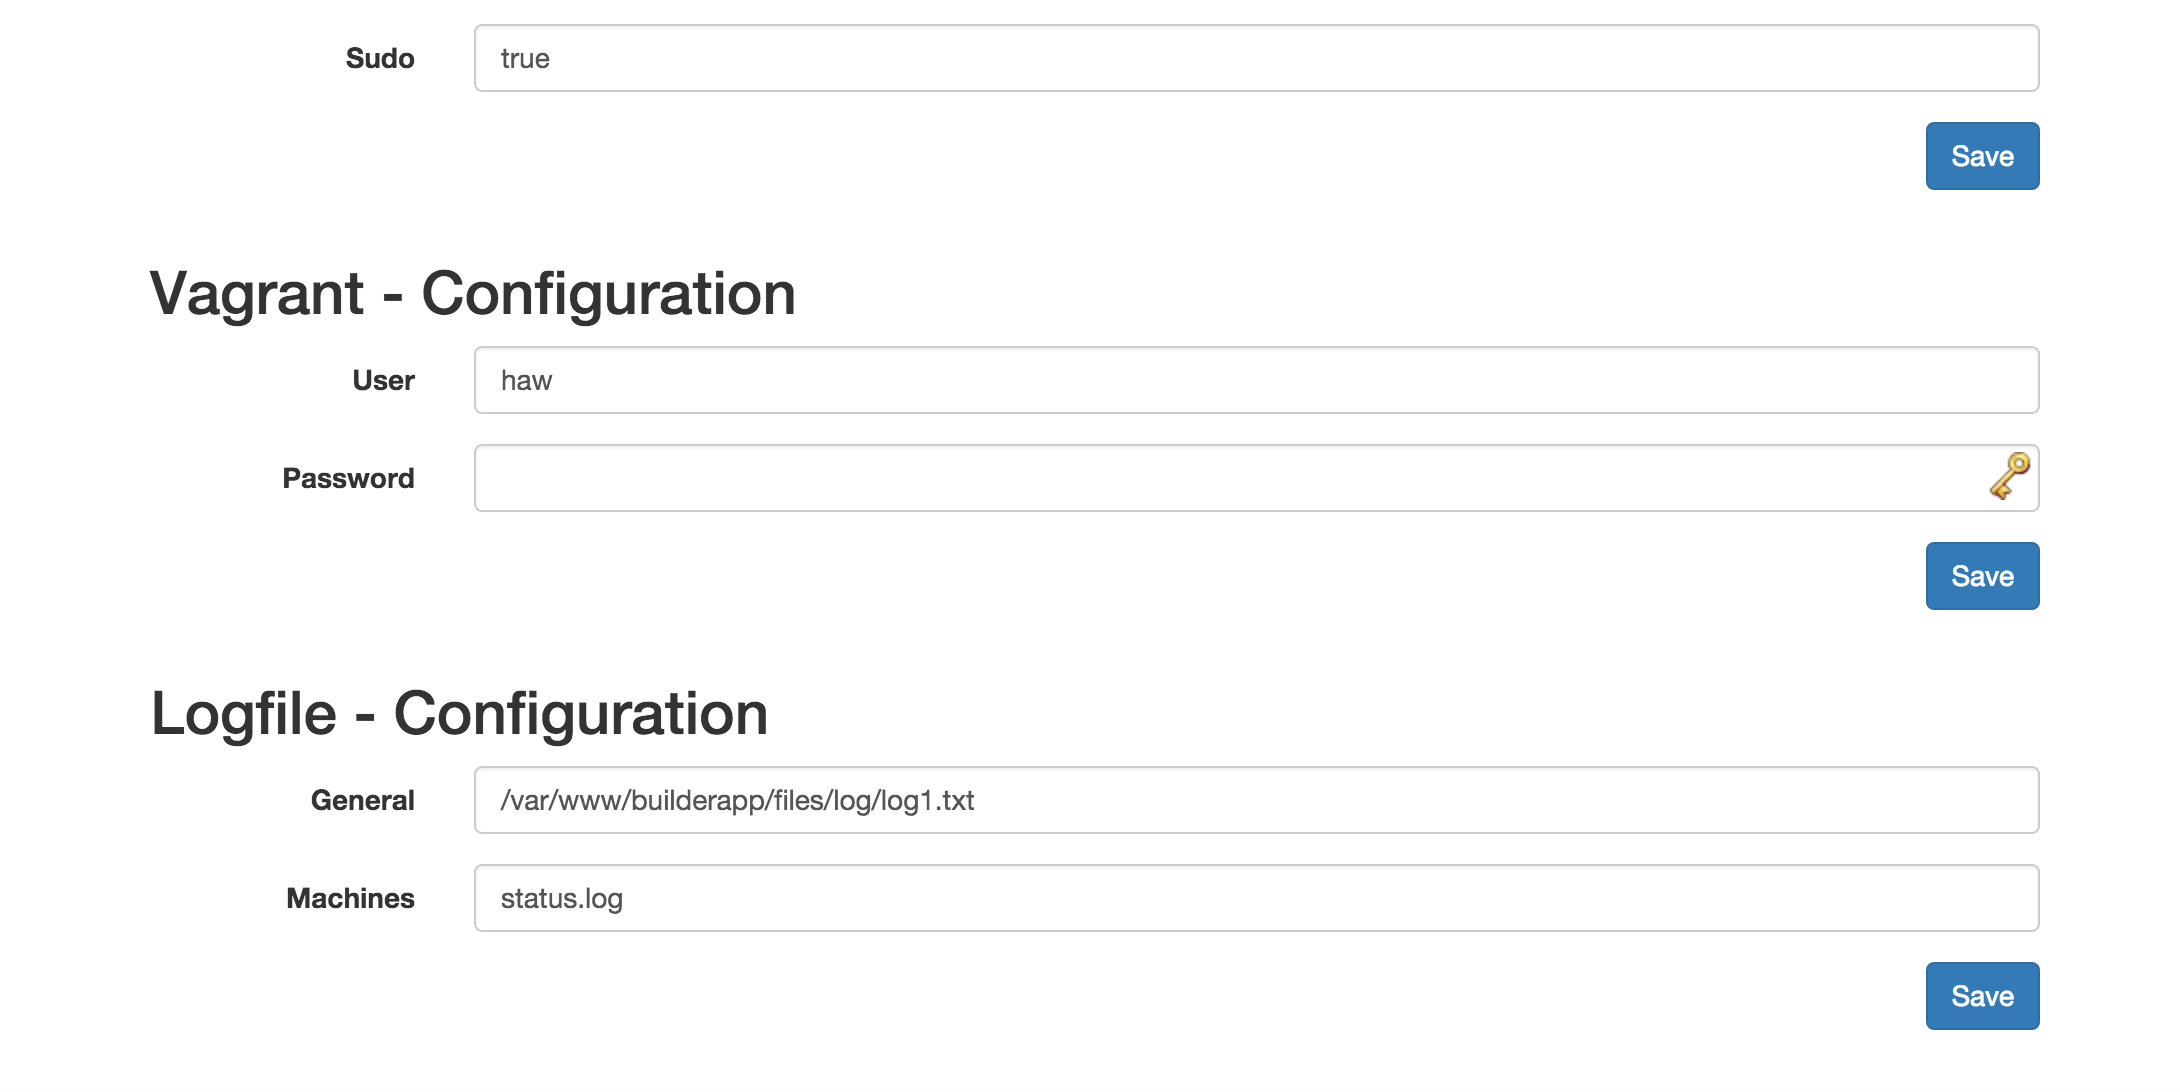
\includegraphics[width=0.9\textwidth]{../Bilder/Anhang/admin_2.png}
  }
  \caption{Administration des VM-Builders (Teil 2)}
	\label{fig:admin2}
\end{figure}
\FloatBarrier

\section*{Software und Packages}\label{sec:SoftwarePackages}
\textcolor{white}{\textbf{Sofwarete und Packages}}
\begin{figure}[htbp]
  \centering
  \fbox{
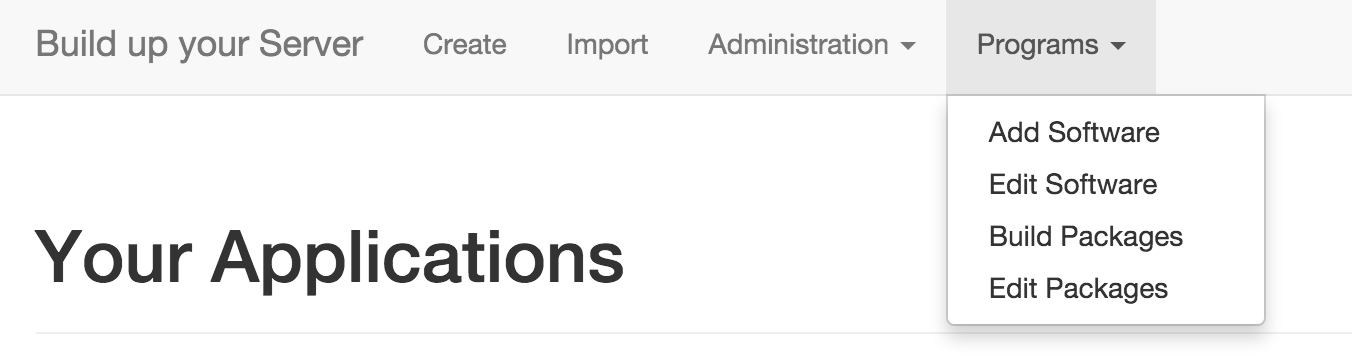
\includegraphics[width=0.9\textwidth]{../Bilder/Anhang/soft_pack.png}
  }
  \caption{Administration von Software und Packages}
	\label{fig:soft_pack}
\end{figure}
\FloatBarrier

\begin{figure}[htbp]
  \centering
  \fbox{
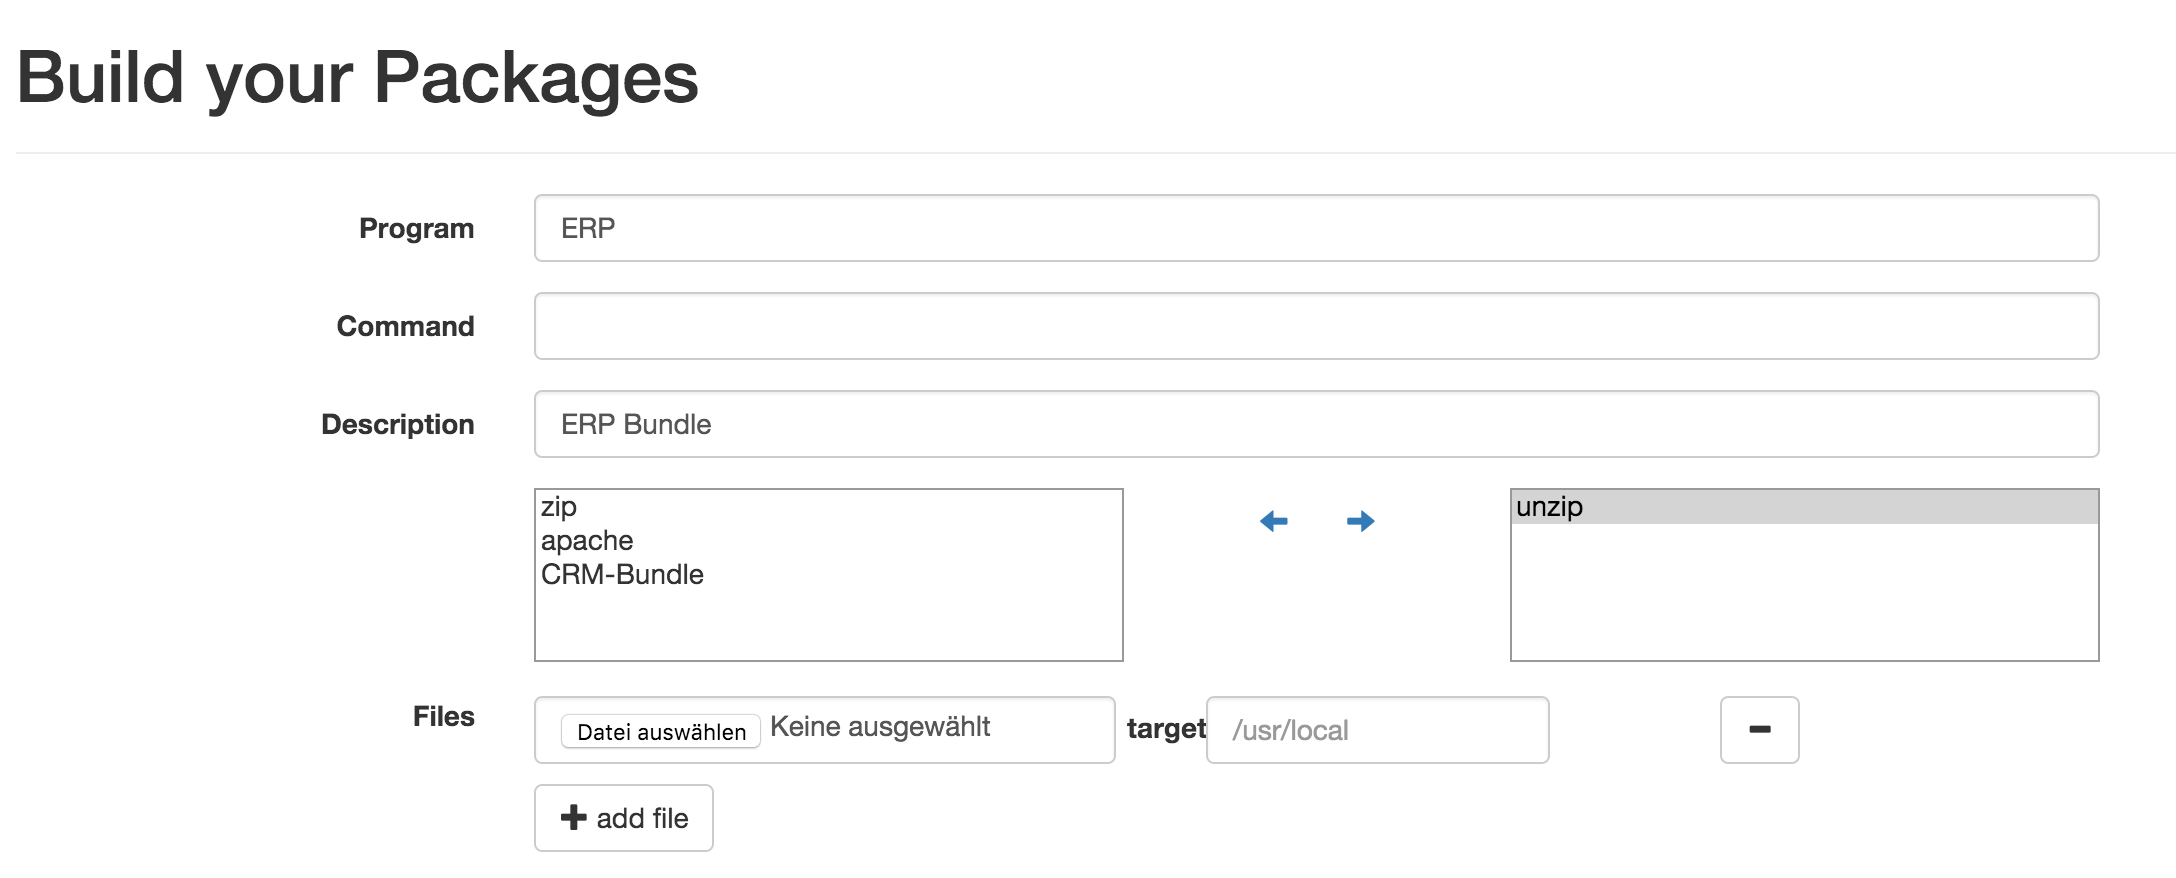
\includegraphics[width=0.9\textwidth]{../Bilder/Anhang/package.png}
  }
  \caption{Erstellung eines Packages}
	\label{fig:pack}
\end{figure}
\FloatBarrier





%%%%
%% add some text to generate a sample document
%%%\setcounter{secnumdepth}{3}
\chapter{Einleitung}
\begin{quote}
	``Es ist nicht zu wenig Zeit, die wir haben, sondern es ist zu viel Zeit, die wir nicht nutzen'' - Lucius Annaeus Seneca, \cite{Apelt200511}
\end{quote}
Seneca formulierte  49 n. Chr. ein Gef"uhl das jeder kennt. Die Zeit die er hat, nicht richtig zu nutzen.
Technische Neuerungen helfen uns unsere Zeit besser zu planen, mehr Zeit in andere Aktivit�ten zu stecken und unsere Priorit�ten zu "uberdenken.
Diese Arbeit besch�ftigt sich mit dem Teil-Aspekt der Informatik, der Virtualisierung von Servern im Entwicklungsumfeld.\newline
... 


\section{Motivation}
\textbf{TODO}
[...]
Die Motivation dieser Ausarbeitung besteht darin, eine Software zu entwickeln, die durch vereinfachte Handhabung und minimaler Einarbeitungszeit, es dem Benutzer erm�glich eine ad-hoc Umgebung zu erstellen, ohne b�rokratischen Aufwand und ohne Grundwissen �ber die darunterliegende Anwendungsstruktur.
Der normalerweise gro�e zeitliche Aufwand soll m�glichst minimiert werden und es Anwendern in Unternehmen und Projekten erleichtern, sich auf die vorhandenen Usecase zu fokussieren und keine Zeit in Aufbau, Installation und Problembehebung investieren zu m�ssen. [...]

\section{Zielsetzung}
Das Ziel der vorliegenden Arbeit ist es, durch inkrementelles und interatives Vorgehen eine Applikation zu modellieren, die den Anwender der Applikation bei dem Aufbau von virtuellen Umgebungen unterst�tzt. Je nach Wunsch des Anwenders, wird nicht nur der Aufbau einer Umgebung vereinfacht, sondern auch die direkte Installation von Programmen veranlasst. Eine Weboberfl�che soll die entsprechenden Optionen zur Verf�gung stellen und dem Anwender durch seine ausgew�hlte Funktion leiten.
Gro�e Konfigurationen oder komplizierte Einstellungen sollen dem Normalanwender abgenommen werden und geschehen im Hintergrund. 
Damit auch ein Sichern oder ein Zur�ckspielen von vorhandenen virtuellen Maschinen m�glich wird, sollten Im- und Exportfunktionen dies untzerst�tzen.
Die Realisierung sollte auf einem zentralen Knotenpunkt stattfinden, um es mehreren Anwendern zu erm�glichen, ihre notwendige Maschine zu erstellen und zu verwalten.
Kernaufgaben sollen Open-Source Anwendungen �bernehmen, die in ihrem Bereich etabliert sind. Ebenfalls im Fokus steht die Leichtigkeit der Konfiguration der auszuw�hlenden Open-Source Anwendung.
Bei der Erstellung der einzelnen Softwarekomponenten ist stehts auf das Prinzip von hoher Koh�sion und loser Kopplung zu achten. Also dem Grad der Abh�ngigkeit zwischen mehrere Hard-/ und Softwarekomponenten, der �nderungen an einzelnen Komponenten erleichtert.
Um auch die Anwendungsoberfl�che unkompliziert zu halten, soll der Anwender mit ein paar Klicks zu seinem Ziel gef�hrt werden. Durch das Vermeiden von unn�tigen Verschachtelungen oder einer Flut an Optionen und Konfigurationen, soll der Anwender in der Applikation einen Helfer f�r seine T�tigkeit finden.
\newline


\begin{comment}


\section{Problemstellung}
%Die Einleitung muss Ihr Thema eingrenzen (und diese Eingrenzung rechtfertigen) und Ihr Erkenntnisinteresse präzisieren und begründen
Virtualisierung hat in vielen Bereichen den physischen Server abgel�st, denn der Finanzielle Aspekt ist f"ur Unternehmen nicht unerheblich. Im Idealfall hei�t der Umstieg auf virtuelle Landschaften gleich weniger Server, was gleichbedeutend mit weniger Stellfl�che ist. Somit auch mit weniger Racks und weniger Verkabelung.\newline
Aufw�ndige Vorplanung von Serverzentren entf�llt, die Kostenplanung der unterschiedlichen Hardware wird minimiert und die Frage, was in ein paar Jahren mit der Hardware passieren soll, wird obsolet.\newline
Gerade im Entwicklungsbereich ist es meist sinnvoller virtuelle Umgebungen zu realisieren, als reale Maschinen aufzubauen. Entwickler haben so die M�glichkeit bei Bedarf sich Abz"uge der Produktionsumgebung zu erstellen oder Fehlerszenarien nachzustellen.\newline
Meist ist dazu die Involvierung des Betriebs-Teams oder des IT-Support notwendig, die nach Priorit�t ihrer Auftragslage, eine gewissen Vorlaufzeit ben�tigen, um die gew�nschte Maschine aufzubauen. \newline
In dem Fall, dass die Firmengr��e es nicht erlaubt, eine eigene Support-Abteilung zu haben, muss die Zeit des jeweiligen Mitarbeiters herhalten, um das Wissen �ber die jeweilige Virtualisierungsl�sung aufzubauen, die gew�nschte Maschine zu erstellen und die Installationen der n�tigen Programme zu realisieren. Der R�ckschluss daraus ist, geringere Produktivit�t in den Kernt�tigkeiten des Mitarbeiters.\newline
Auch wenn die Softwarebranche eine Vielfalt an M�glichkeiten bereitstellt, sind diese entweder in ihrer Struktur �berdimensioniert, um sie in der Anwendung schnell zu erlernen, oder komplex in ihrer Konfiguration in Bezug auf Automatisierungen und/oder Provisionierungen.

\end{comment}

\section{Themenabgrenzung}
Diese Arbeit greift bekannte und etablierte Softwareprodukte auf und nutzt diese in einem zusammenh�ngenden Kontext. Dabei werden die verwendeten Softwareprodukte nicht modifiziert, sondern f�r eine vereinfachte Benutzung durch eigene Implementierungen kombiniert und mit einem Benutzerinterface versehen, welches die Abl�ufe visualisiert und dem Benutzer die Handhabung vereinfacht.
Die vorzunehmenden Implementierungen greifen nicht in den Ablauf der jeweiligen Software ein, sondern vereinfacht das Zusammenspiel der einzelnen Anwendungen.



\section{Struktur der Arbeit}
[...]

\chapter{Grundlagen}
[...]
%Dieses Kapitel gibt einen Einblick in die Grundlagen der Virtualisierung.
%Dieses Kapitel soll die Einblick in die Grundlagen der Virtualisierung geben.
%Zun�chst wird erl�utert, was Virtualisierung ist, dann werden Begrifflichkeiten gekl�rt sowie Vor- und Nachteile begutachtet.

\section{Grundlagen der Virtualisierung}
F�r den Begriff Virtualisierung existiert keine allgemeing�ltige Definition. In der Regel wird damit der parallele Einsatz mehrerer Betriebssysteme beschrieben oder detailierter, das Ressourcen zu einer logischen Schicht zusammengefasst werden und dadurch deren Auslastung optimiert wird. So kann die logische Schicht bei Aufforderung ihre Ressourcen automatisch zur Verf�gung stellen. 
Das Prinzip dahinter ist die Verkn�pfung von Servern, Speichern und Netzen zu einem virtuellen Gesamtsystem.
Daraus k�nnen sich dar�ber liegende Anwendungen direkt und bedarfsgerecht ihre Ressourcen beziehen.\newline
Grunds�tzlich unterscheidet man zwischen 
\begin{enumerate}
\item \textbf{Virtualisierung von Hardware}\newline
die sich mit der Verwaltung von Hardware-Ressourcen besch�ftigt und
\item \textbf{Virtualisierung von Software}\newline 
die sich mit der Verwaltung von Software-Ressourcen, wie z.B. Anwendungen und Betriebssystemen besch�ftigt.
\end{enumerate}
[\cite{Bengel200806}]



\subsection{Virtuelle Maschine}\label{subsec:VirtuelleMaschine}
Eine virtuelle Maschine ist nach Robert P. Goldberg
\begin{quote}
\textit{'a hardware-software duplicate of a real existing computer system in
which a statistically dominant subset of the virtual processor's
instructions execute directly on the host processor in native mode'} [\cite{SiegertBaumgarten200612}]
\end{quote} 
W�rtlich �bersetzt ist also eine virtuelle Maschine ein Hardware-/Software-Duplikat eines real existierenden Computersystems, in dem eine statistisch dominante Untermenge an virtuellen Prozessoren, Befehle im Benutzer-Modus auf dem Host-Prozessor ausf�hren.
Dieses Duplikat kann als Software-Container betrachtet werden, der einen vollst�ndigen Satz an emulierten Hardwareressourcen, dem Gastbetriebssystem und entsprechenden Anwendungen besteht. Durch die Containerstruktur wird eine Kapselung hervorgerufen, die es erm�glicht mehrere virtuelle Maschinen komplett unabh�ngig auf einem Hostsystem zu installieren und laufen zu lassen. Ist eine virtuelle Maschine fehlerhaft oder nicht mehr erreichbar, betrifft dies nicht automatisch die restlichen parallel laufenden Maschinen und stellt damit einen der charakteristischen Vorteile von virtuellen Maschinen dar. Die Verf�gbarkeit. Backup-Systeme oder mehrere Instanzen einer Applikationen k�nnen so unabh�ngig auf einem Host ausgef�hrt werden, ohne sich gegegnseitig zu beeinflussen. Durch den struktuellen Aufbau einer virtuellen Maschine, ist es ebenfalls m�glich, eine Maschine nach den eigenen W�nschen zu erstellen und diese im Weiteren zu replizieren.\newline
Virtuelle Maschinen k�nnen ohne gr��eren Aufwand verschoben, kopiert und zwischen Hostservern neu zugeteilt werden, um die Hardware-Ressourcen-Auslastung zu optimieren. Administratoren k�nnen auch die Vorteile von virtuellen Umgebungen f�r einfache Backups, Disaster Recovery, neue Deployments und grundlegenden Aufgaben der Systemadministration nutzen, da das Wiederherstellen aus Speicherpunkten oder gespeicherten Abz�gen, innerhalbt von Minuten zu realisieren ist.\newline


\subsection{Gastbetriebssystem}\label{subsec:Gastbetriebssystem}
Ein �bliches Betriebssystem wird im privilegierten Prozessor-Modus ausgef�hrt (Auch Kernel-Mode genannt). Dies bef�higt es, die absolute Kontrolle �ber die vorhandenen Ressourcen zu gewinnen. Alle Anwendungen, die auf dem Betriebssystem laufen, werden im sogenannten Benutzer-Modus ausgef�hrt. Die Privilegien im Benutzer-Modus sind allerdings relativ eingeschr�nkt. Ein direkter Zugriff wird nur sehr selten und unter genau kontrollierten Bedingungen gestattet. Dies hat den Vorteil, dass kein Programm z. B. durch einen Fehler das System zum Absturz bringen kann. (\cite{Reuther2014})\newline
Eine virtuelle Maschine (siehe \ref{subsec:VirtuelleMaschine}) l�uft als normaler Benutzer-Prozess im Benutzer-Modus, was zur Folge hat, dass das dort installierte Betriebssystem, das Gastbetriebssystem, folglich nicht den privilegierten Prozessor-Modus nutzen kann, wie es ein nicht virtualisiertes Betriebssystem k�nnte. Da weder die Anwendungen noch das entsprechende Gastbetriebssystem Kentniss dadr�ber haben, dass sie in einer virtuellen Maschine laufen, m�ssen ausgef�hrte Instruktionen, die den Prozessor-Modus erfordern, entsprechend anders gehandhabt werden. Dies ist unter anderem die Aufgabe des Hypervisors (siehe \ref{subsec:Hypervisor}).


\begin{center}
 \begin{minipage}{\linewidth}
	\centering
	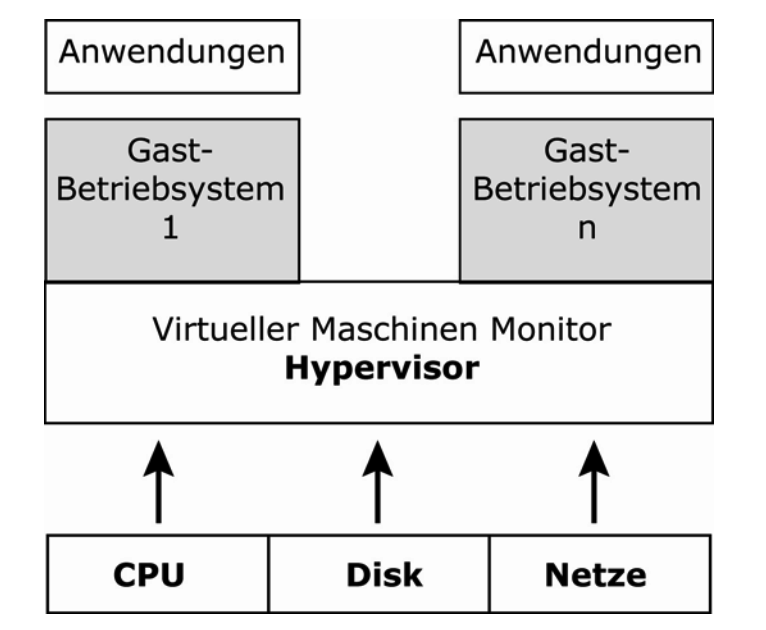
\includegraphics[scale=0.4]{../Bilder/BSVirtualisierung.png}%
	\captionof{figure}[Betriebssystemvirtualisierung]{Betriebssystemvirtualisierung [\cite{SiegertBaumgarten200612}]}%
	\label{fig:Betriebssystemvirtualisierung}% 
 \end{minipage}
\end{center}


\subsection{Hypervisor}\label{subsec:Hypervisor}
Der Name des Hypervisors kann von Hersteller zu Hersteller variieren. Bei Microsoft z.B.  wird er Hyper-V genannt und bei VMware als ESXi bezeichnet.
Der Hypervisor, oder in der Literatur auch VMM (Virtual Machine Monitor) genannt, ist die sogenannte abstrahierende Schicht zwischen der tats�chlich vorhanden Hardware und den ggf. mehrfach existierenden Betriebssystemen. Siehe \ref{fig:Betriebssystemvirtualisierung}.
Seine prim�re Aufgabe ist die Verwaltung der Host-Ressourcen und deren Zuteilung bei Anfragen der Gastsysteme. L�sen Instruktionen, oder Anfagen eines Gastbetriebssystems eine CPU-Exception aus, weil diese im Benutzer-Modus ausgef�hrt werden, f�ngt der Hypervisor diese auf und emmuliert die Ausf�hrung der Instruktionen (trap and emulate). Die Ressourcen des Hostsystems werden derart verwaltet, dass diese bedarfsgerecht zur Verf�gung stehen, egal ob ein oder mehrere Gastsysteme laufen. Zudem z�hlt unter anderem E/A-Zugriffe (insbesondere Hardwarezugriffe), Speichermanagement, Prozesswechsel und System-Aufrufe.\newline
Den Hypervisor kann man in zwei verschiedene Typen kategorisiert.
\begin{description}
\item  [Typ 1 Hypervisor]\hfill \\
arbeitet direkt auf der Hardware und ben�tigt somit kein Betriebssystem, welches zwischen ihm und der Hardware liegt. Alle dar�ber liegenden virtuelle Maschinen laufen in sogenannten Domains. Weder der Hypervisor noch die anderen Domains sind f�r die jeweilige Domain sichtbar. Die Verwaltung der laufenden Domains wird durch eine priviligierte Domain geregelt, die in der Dom0 l�uft. Dadurch hat die priviligierte Domain die M�glichkeit andere Domains zu starten, stoppen und zu verwalten. \newline
Der Hypervisor Type-1 verf�gt selbst �ber die n�tigen Ger�tetreiber, um den virtuellen Maschinen CPU, Speicher und I/O zur Verf�gung zu stellen. Durch die wegfallende Schicht, das nicht ben�tigte Betriebssystem, gewinnt der Hypervisor Typ 1 an Performance und spart am Ressourcenverbrauch. Siehe Abbildung [\ref{fig:KlassifizierungHypervisor}.a].

\item  [Typ 2 Hypervisor]\hfill \\
l�sst durch seine Bezeichnung als 'Hosted' erahnen, dass der Unterschied zu Typ 1 darin besteht, dass er auf einem Hostsystem aufsetzt. Also eine Schicht implementiert sein muss, die zwischen dem Hypervisor und der Hardware liegt. Siehe Abbildung [\ref{fig:KlassifizierungHypervisor}.b].\newline
Diese Schicht wird durch ein Betriebssystem realisiert, das dem Hypervisor den Zugang zur Hardware durch die eigenen Hardwaretreiber erm�glicht.
Ist ein Betriebssystem mit einer Hardware kompatibel, ist transitiv gesehen, der Hypervisor ebenfalls mit installier- und ausf�hrbar. Dies vereinfacht die Installation gegen�ber dem Hypervisor Typ 1. \newline
Aus Implementierungssicht gibt es f�r beide Hypervisoren Vor- und Nachteile.
F�r einige Bereiche ist die Anforderung eines Betriebssystems nur von Vorteil.
Vor allem wenn es um um Hardware- und Treiber-Kompatibilit�t, Konfigurationsflexibilit�t und vertraute Management-Tools geht.\newline
Auf der anderen Seite kann genau das zum Nachteil ausgelegt werden.
Es entsteht nicht nur ein h�herer Management-Aufwand um das Betriebssystem zu konfigurieren und zu verwalten, auch die Performance und der Sicherheitsaspekt leiden unter dieser zus�tzlichen Schicht. 
\end{description}
\begin{figure} 
    \subfigure[Bezeichnung der linken Grafik]{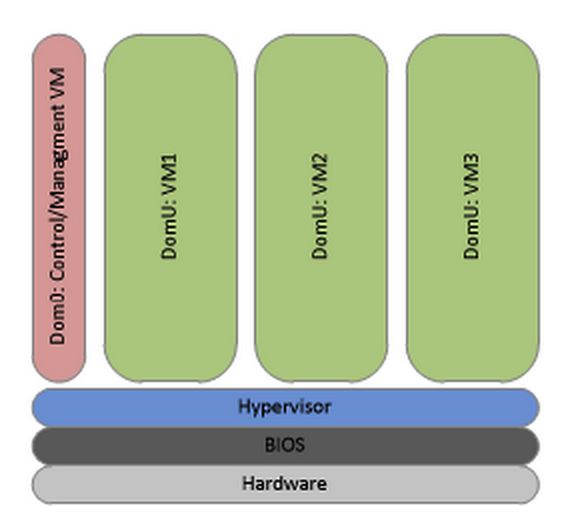
\includegraphics[width=0.49\textwidth]{../Bilder/Hypervisor1.png}} 
    \subfigure[Bezeichnung der rechten Grafik]{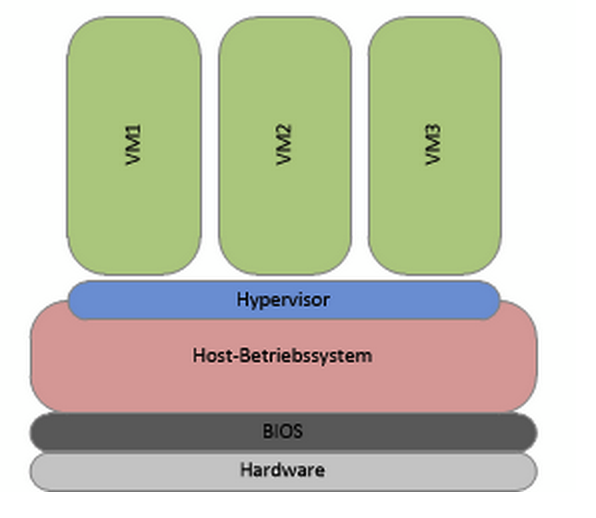
\includegraphics[width=0.49\textwidth]{../Bilder/Hypervisor2.png}} 
\label{fig:KlassifizierungHypervisor}%
\caption{Hypervisor Typ 1 und 2} 
\end{figure} 

\section{Provisioning/Konfigurationsmanagement}\label{subsec:Provisioning}
\textbf{TODO: WELCHER BEGRIFF IST BESSER?}\newline
Die Hauptaufgabe eines Konfigurationsmanagement-Systems, im folgenden nur noch KMS genannt, ist es, eine zuvor definierte Zustandsbeschreibung eines Hosts umzusetzen. Dies kann das Installieren von Softwarepaketen bedeuten, starten oder beenden von Diensten oder  Konfigurationen erstellen/anpassen/entfernen zu lassen.
In der Regel verwenden KMS eigene Agenten auf den Zielsystemen, �ber die die Kommunikation l�uft und die Zustandsbeschreibung realisiert wird. Neuere Anwendungen wie 'Ansible' aus Kapitel \ref{subsec:Ansible}, die Konfigurationsmanagement unterst�tzen, ben�tigen diese Agenten nicht mehr und realisieren die Kommunikation �ber eine SSH-Schnittstelle.
Pull-basierte Tools, wie beispielsweise 'Puppet', fragen in regelm�ssigen Abst�nden ein zentrales Konfigurations-Repository ab, in dem die jeweils aktuelle Zustandsbeschreibung der Maschine gespeichert ist und sorgt daf�r, dass die �nderungen auf dem Client ausgef�hrt werden.
Es spielt keine Rolle, ob der Zielclient eine virtuelle Maschine ist oder eine standard Maschine ist. KMS sind in der Regel dazu f�hig ganze Gruppen an Rechner parallel zu bearbeiten und die entsprechenden Zustandsbeschreibungen umzusetzen. 
Bei dem im oberen Abschnitts bereits genannten Beispiel 'Ansible', k�nnen mehrere Rechner simpel in Inventory-Dateien als Gruppen zusammengefasst werden, die dann jeweils durch 'Ansible' angesprochen werden k�nnen um entsprechende St�nde an Zustandsbeschreibungen dort auszuliefern. Siehe \ref{lst:InventoryDatei}

\begin{lstlisting} [caption={Beispiel Inventory-Datei}\label{lst:InventoryDatei},captionpos=t] 
[atomic]
 192.168.100.100
 192.168.100.101
[webserver]
 192.168.1.110
 192.168.1.111
 \end{lstlisting}

%Quelle: http://www.admin-magazin.de/Online-Artikel/Konfigurationsmanagement-mit-Ansible
\begin{comment}
\section{Begriffserkl�rung}
Im Verlauf dieser Arbeit werden Begrifflichkeiten verwendet, die im Vorfeld zu kl�ren sind.\newline
	\begin{enumerate}
		\item \textbf{Provisioning / Provisioner}\newline
\textit{Provisioning} ist ein Aspekt der Informatik, in dem es darum geht, den richtigen Personen zur richtigen Zeit effektiv Ressourcen zur Verf�gung zu stellen.
\textit{Provisioner} helfen bei der Softwareverteilung auf gew�nschte Maschinen, Ad-hoc Kommando-Ausf�hrung und Konfigurationsmanagement.
In dieser Arbeit bezieht sich der Begriff \textit{Provisioning} auf die automatisierte Softwareverteilung, die mit dem Aufbau einer Entwicklungsumgebung verbunden ist.\newline
		\item \textbf{Entwicklungsumgebung}\newline
IDE's (integrated development environment) sind Entwicklungsumgebungen, die den Entwickler unterst�tzen, Quellcode zu schreiben und zu bearbeiten. Die g�ngigsten IDE's unterst�tzen meist mehrere Programmiersprachen und helfen dem Entwickler mit n�tzlichen Funktionen, wie  z.B. das aufzeigen von Fehlern im Quelltext. Entwicklungsumgebungen sind in vielen F�llen auch PC's / Server / virtuelle Maschinen, die zum Entwickeln installiert und bereitgestellt werden.
Dort k�nnen neue Funktionalit�ten ausprobiert werden und das bestehende System testweise erweitert werden, ohne in die Produktionslandschaft einzugreifen.
In den folgenden Texten wird der Begriff \textit{Entwicklungsumgebung} als Synonym f�r eine virtuelle Maschine benutzt, die dem Anwender die Freiheit gibt, unkompliziert M�glichkeiten auszutesten und neues auszuprobieren.\newline
		\item \textbf{Aufbau einer Maschine}\newline
\textit{Aufbau einer Maschine} beinhaltet immer das automatische Erstellen und Konfigurieren einer virtuellem Maschine mit Hilfe von VirtualBox und Vagrant.
Das Resultat ist eine virtuelle Maschine mit der Basisinstallation von Ubuntu (32Bit / 64Bit) und \textbf{MEHR INFOS ZU DEM SYSTEM}.
Durch die M�glichkeit des Provisioning kann die Basisinstallation mit Software erg�nzt und Befehle auf der Maschine ausgef�hrt werden.

\item \textbf{Maschinenkonfiguration}\newline
F�r den Aufbau einer Maschine werden zwei wesentliche Konfigurationsdateien erstellt.
Diese werden f�r den Aufbau der virtuelle Maschine selbst ben�tigt und f�r das ggf. gew�nschte Provisioning. Der Begriff \textit{Maschinenkonfiguration} beschreibt im folgenden immer das Vorhandensein beider Dateien. 
\end{enumerate}
\end{comment}


%%\subfile{Einleitung}



%\lipsum


%%%%

%% appendix if used
%%\appendix
%%\typeout{===== File: appendix}
%%\include{appendix}

% bibliography and othjer stuff
\backmatter

\typeout{===== Section: literature}
%% read the documentation for customizing the style
\bibliographystyle{dinat}
\listoffigures
\lstlistoflistings
\bibliography{literatur}


\typeout{===== Section: nomenclature}
%% uncomment if a TOC entry is needed
%%\addcontentsline{toc}{chapter}{Glossar}
\renewcommand{\nomname}{Glossar}
\clearpage
\markboth{\nomname}{\nomname} %% see nomencl doc, page 9, section 4.1
\printnomenclature

%% index
\typeout{===== Section: index}
\printindex

\HAWasurency



\end{document}
